\documentclass[12pt,oneside,openright,a4paper]{cpe-english-project}
\usepackage{placeins}
\usepackage{polyglossia}
\setdefaultlanguage{english}
\setotherlanguage{thai}
\newfontfamily\thaifont[Script=Thai,Scale=1.23]{TH Sarabun New}
\defaultfontfeatures{Mapping=tex-text,Scale=1.0,LetterSpace=0.0}
\setmainfont[Scale=1.0,LetterSpace=0,WordSpace=1.0,FakeStretch=1.0]{Times New Roman}
\emergencystretch=10pt
%\XeTeXlinebreaklocale "th_TH"	
%\XeTeXlinebreakskip = 0pt plus 1pt
%\setmathfont(Digits)[Scale=1.0,LetterSpace=0,FakeStretch=1.0]{Times New Roman}


%%%%%%%%%%%%%%%%%%%%%%%%%%%%%%%%%%%%%%%%%%%%%%%%%%%%%%%%%%%%%%%%%%%
% Customize below to suit your needs 
% The ones that are optional can be left blank. 
%%%%%%%%%%%%%%%%%%%%%%%%%%%%%%%%%%%%%%%%%%%%%%%%%%%%%%%%%%%%%%%%%%%
% First line of title
\def\disstitleone{DENTAL AI CHATBOT FOR DIAGNOSTICS AND POST-SURGERY CARE}   
% Your first name and lastname
\def\dissauthor{MR. CHANON KHANIJOH}   % 1st member
%%% Put other group member names here ..
\def\dissauthortwo{MR. PECHDANAI SAEPONG}   % 2nd member (optional)
\def\dissauthorthree{MS. FASAI SAE-TAE}   % 3rd member (optional)
\def\dissauthorID{63070503408}              % Author of dissertation
\def\dissauthortwoID{63070503434}              % Author of dissertation
\def\dissauthorthreeID{63070503436}   
\def\dissauthorEMAIL{chanon.kha@mail.kmutt.ac.th}              % Author of dissertation
\def\dissauthortwoEMAIL{pechdanai.sp@mail.kmutt.ac.th}              % Author of dissertation
\def\dissauthorthreeEMAIL{fasai.sae@mail.kmutt.ac.th}  


% The degree that you're persuing..
\def\dissdegree{Bachelor of Engineering} % Name of the degree
\def\dissdegreeabrev{B.Eng} % Abbreviation of the degree
\def\dissyear{2023}                   % Year of submission
\def\thaidissyear{2566}               % Year of submission (B.E.)

%%%%%%%%%%%%%%%%%%%%%%%%%%%%%%%%%%%%%%%%%%%%
% Your project and independent study committee..
%%%%%%%%%%%%%%%%%%%%%%%%%%%%%%%%%%%%%%%%%%%%
\def\dissadvisor{Dr. Unchalisa Taetragool , Ph.D.}  % Advisor
%%% Leave it empty if you have no Co-advisor
\def\disscoadvisor{Dr. Vorapat Trachoo, D.D.S., M.D.}  % Co-advisor
%%% Leave it empty if you have no Co-advisor 2
\def\disscoadvisortwo{Dr. Kritsasith Warin, D.D.S.}  % Co-advisor 2

\def\worktype{Project} %%  Project or Independent study
\def\disscredit{3}   %% 3 credits or 6 credits


\def\fieldofstudy{Computer Engineering} 
\def\department{Computer Engineering} 
\def\faculty{Engineering}
 
\def\appendixnames{Appendix} %%% Appendices or Appendix

% Change the line spacing here...
\linespread{1.15}

%%%%%%%%%%%%%%%%%%%%%%%%%%%%%%%%%%%%%%%%%%%%%%%%%%%%%%%%%%%%%%%%
% End of personal customization.  Do not modify from this part 
% to \begin{document} unless you know what you are doing...
%%%%%%%%%%%%%%%%%%%%%%%%%%%%%%%%%%%%%%%%%%%%%%%%%%%%%%%%%%%%%%%%


%%%%%%%%%%%% Dissertation style %%%%%%%%%%%
%\linespread{1.6} % Double-spaced  
%%\oddsidemargin    0.5in
%%\evensidemargin   0.5in
%%%%%%%%%%%%%%%%%%%%%%%%%%%%%%%%%%%%%%%%%%%
%\renewcommand{\subfigtopskip}{10pt}
%\renewcommand{\subfigbottomskip}{-5pt} 
%\renewcommand{\subfigcapskip}{-6pt} %vertical space between caption
%                                    %and figure.
%\renewcommand{\subfigcapmargin}{0pt}

\renewcommand{\topfraction}{0.85}
\renewcommand{\textfraction}{0.1}

\newtheorem{theorem}{Theorem}
\newtheorem{lemma}{Lemma}
\newtheorem{corollary}{Corollary}

\def\QED{\mbox{\rule[0pt]{1.5ex}{1.5ex}}}
\def\proof{\noindent\hspace{2em}{\itshape Proof: }}
\def\endproof{\hspace*{\fill}~\QED\par\endtrivlist\unskip}
%\newenvironment{proof}{{\sc Proof:}}{~\hfill \blacksquare}
%% The hyperref package redefines the \appendix. This one 
%% is from the dissertation.cls
%\def\appendix#1{\iffirstappendix \appendixcover \firstappendixfalse \fi \chapter{#1}}
%\renewcommand{\arraystretch}{0.8}
%%%%%%%%%%%%%%%%%%%%%%%%%%%%%%%%%%%%%%%%%%%%%%%%%%%%%%%%%%%%%%%%
%%%%%%%%%%%%%%%%%%%%%%%%%%%%%%%%%%%%%%%%%%%%%%%%%%%%%%%%%%%%%%%%


\begin{document}
\pdfstringdefDisableCommands{%
\let\MakeUppercase\relax
}
\begin{center}
  
\includegraphics[width=2.8cm]{Image/KMUTT_Logo.png}
\end{center}
\vspace*{-1cm}


\maketitlepage 
\makesignaturepage 

%%%%%%%%%%%%%%%%%%%%%%%%%%%%%%%%%%%%%%%%%%%%%%%%%%%%%%%%%%%%%
%%%%%%%%%%%%%%%% ToC, List of figures/tables %%%%%%%%%%%%%%%%
%%%%%%%%%%%%%%%%%%%%%%%%%%%%%%%%%%%%%%%%%%%%%%%%%%%%%%%%%%%%%
% The three commands below automatically generate the table 
% of content, list of tables and list of figures
\tableofcontents                    
\listoftables
\listoffigures                      

%%%%%%%%%%%%%%%%%%%%%%%%%%%%%%%%%%%%%%%%%%%%%%%%%%%%%%%%%%%%%%
%%%%%%%%%%%%%%%%%%%%% List of symbols page %%%%%%%%%%%%%%%%%%%
%%%%%%%%%%%%%%%%%%%%%%%%%%%%%%%%%%%%%%%%%%%%%%%%%%%%%%%%%%%%%%
% You have to add this manually..
\listofsymbols
\begin{flushleft}
\begin{tabular}{@{}p{0.07\textwidth}p{0.7\textwidth}p{0.1\textwidth}}
\textbf{SYMBOL}  & & \textbf{UNIT} \\[0.2cm]
% $\alpha$ & Test variable\hfill & m$^2$ \\
% $\lambda$ & Interarival rate\hfill &  jobs/second\\
% $\mu$ & Service rate\hfill & jobs/second\\
\end{tabular}
\end{flushleft}
%%%%%%%%%%%%%%%%%%%%%%%%%%%%%%%%%%%%%%%%%%%%%%%%%%%%%%%%%%%%%%
%%%%%%%%%%%%%%%%%%%%% List of vocabs & terms %%%%%%%%%%%%%%%%%
%%%%%%%%%%%%%%%%%%%%%%%%%%%%%%%%%%%%%%%%%%%%%%%%%%%%%%%%%%%%%%
% You also have to add this manually..
\listofvocab
\begin{flushleft}
\begin{tabular}{@{}p{1in}@{=\extracolsep{0.5in}}p{0.73\textwidth}}
AI & Artificial Intelligence \\
API & Application Programming Interface \\
BERT & Bidirectional Encoder Representations from Transformers \\
CSS & Cascading Style Sheet \\
DL & Deep Learning \\
DOM & Document Object Model \\
DSRM & Design Science Research Methodology \\
DT & Decision Tree \\
HTML & Hypertext Markup Language \\
ID & Identification \\
JS & JavaScript \\
ML & Machine Learning \\
mDeBERTa & Multilingual Decoding-enhanced BERT with disentangled attention \\
NLP & Natural Language Processing \\
NN & Neural Network \\
ODM & Object Document Modelling \\
OPD & Outpatient Department \\
RF & Random Forest \\
RoBERTa & Robustly Optimized BERT Approach \\
SDK & Software Development Kit \\
SQL & Structured Query Language \\
TS & TypeScript \\
UI & User Interface \\
UX & User Experience \\
WWW & World Wide Web \\

\end{tabular}
\end{flushleft}

%\setlength{\parskip}{1.2mm}

%%%%%%%%%%%%%%%%%%%%%%%%%%%%%%%%%%%%%%%%%%%%%%%%%%%%%%%%%%%%%%%
%%%%%%%%%%%%%%%%%%%%%%%% Main body %%%%%%%%%%%%%%%%%%%%%%%%%%%%
%%%%%%%%%%%%%%%%%%%%%%%%%%%%%%%%%%%%%%%%%%%%%%%%%%%%%%%%%%%%%%%


\chapter{Introduction}
  \section{Keywords}
    \qquad Keywords: Oral Surgery, Dentistry, Diagnose, Follow-up, Artificial Intelligence, Chatbot, Machine Learning, Natural Language Processing

  \section{Problem Statement}
    \subsection{Problem Statement and Motivation}
      \qquad Individuals seeking healthcare in today's world often run into a number of challenges while attempting to acquire correct information regarding their symptoms and appropriate treatment. Many patients have minor illnesses or symptoms that might not necessarily require immediate medical attention from a doctor. Nevertheless, these individuals usually resort to clinics or hospitals for a diagnosis as there is a lack of information and assistance available. \par
      \qquad This rise in patient visits not only places a considerable burden on healthcare facilities but also results in financial implications for patients themselves. The associated costs, such as consultation fees, diagnostic tests, and travel expenses, can impose an unreasonable financial strain on individuals. Moreover, this increased demand for medical attention has contributed to an imbalance in the doctor-to-patient ratio, affecting the overall quality of healthcare services provided. According to the National Statistical Office, the ratio of doctor-to-patient ratio is 1 to 8,057.\par
      \qquad Furthermore, the challenges do not cease once treatment is initiated. After receiving medical care, many patients still have many concerns about their health conditions. Many patients desire prompt answers to their worries about their conditions. In addition to these concerns, patients often have recurring questions, commonly categorized as frequently asked questions (FAQs).\par
      \qquad Regrettably, doctors and medical staff find themselves overwhelmed by the immense workload caused from the increased patient influx. As they aim to deliver quality care and diagnosis, they may have limited time and resources to respond satisfactorily to the patients.\par
      \qquad To address these pressing issues and enhance the healthcare experience for both patients and healthcare providers, we were motivated to develop an application that can effectively address these issues. The application will have the capability to diagnose common diseases and answer frequently asked questions from the patient's symptoms. Additionally, it will feature a chatbot designed to follow up on patient conditions after surgery.\par


    \subsection{Potential Benefits}
      \qquad The purpose of this dental application is to reduce frequently asked questions from patients regarding oral symptoms or diseases and also help with post-surgery follow-up thus reducing the workload of the dentist and medical staff. Dentists can use the extra time they gain to concentrate on patients who require more extensive care.\par
      \qquad In addition to the benefits that doctors receive from this application, patients and the general public also get their benefit as they have immediate access to oral diagnosis and knowledge. Since patients can understand their symptoms and get guidance on simple treatments, this helps to decrease needless doctor visits. Moreover, it can benefit patients by decreasing the expense of visiting the doctor to get a diagnosis. Another benefit that patients receive is continuous monitoring of their symptoms, which allows their doctor to be informed of any unexpected post-surgery problems.\par

  \section{Objectives}
    \begin{itemize}
      \item To acquire the knowledge and skills necessary for developing an AI-powered chatbot. 
      \item To build a chatbot specialized in providing accurate answers to specific dental questions.
      \item To reduce doctors and staff by minimizing repeated questions and explanations from patients.
    \end{itemize}

  \section{Expected Result}
    \qquad This project aims to develop a chatbot utilizing advanced natural language processing and machine learning techniques to be able to address frequently asked questions related to oral surgeries and be able to perform post-surgery follow-up. The chatbot is expected to provide an accurate response. \par  

  \section{Scope of Work}
    \qquad The scope of this project involves the development of a chatbot designed to address frequently asked questions related to oral surgeries and provide post-surgery follow-up support. The chat bot will utilize natural language processing (NLP) and machine learning algorithms. The primary functions of the chatbot includes answering queries about each surgery, performing post-surgery follow-up, offering guidance and suggestions. Our primary focus will be on 4 specific surgical operations: Tooth Extraction, Wisdom Tooth Removal, Periodontal Surgery, Dental Implant Surgery. \par
    \qquad The final deliverable of this project will be a fully functional chatbot integrated into a web application, able to handle a range of frequently asked questions and perform post-surgery follow-ups. The project involves extensive research into relevant dentistry information, the development and training of machine learning models for question answering, and the design and implementation of the user interface. A usability test will be conducted to assess the effectiveness and user-friendliness of the chatbot and the associated web application. \par

  \section{Project Schedule}
    \subsection{Semester 1}
      \begin{enumerate}
        \item Proposal
          \begin{itemize}
            \item Discuss Project with Advisors
            \item Kick-off meeting
            \item Write Project Idea
            \item Write Proposal Report
            \item Make Proposal Presentation          
          \end{itemize}
        \item Project Planning
          \begin{itemize}
            \item Collect Requirement
            \item Plan Task Schedule          
          \end{itemize}
        \item Learning and Research
          \begin{itemize}
            \item Research on Methodology
            \item Research On Oral Symptoms and FAQ
            \item Research on Related Paper
            \item Study 4 Specific Oral Surgical Operations
            \item Study Post Surgery Follow-Up Procedure
          \end{itemize}
        \item Collect Data
          \begin{itemize}
            \item Prepare for Data Collecting
            \item Data Collecting
            \item Clean Data                 
          \end{itemize}
        \item Design and Data Preparation
          \begin{itemize}
            \item Make Use Case Diagram
            \item Make Architecture Diagram
            \item Design UX/UI
            \item Design AI Design
            \item Make Navigation Map                  
          \end{itemize}
        \item Implementation
          \begin{itemize}
            \item Select an Appropriate State-of-the-art AI Model
            \item Select an Appropriate Chatbot Framework 
            \item Select an Appropriate Front End Framework                 
          \end{itemize}
        \item Final Report
          \begin{itemize}
            \item Write Final Report
            \item Make Final Presentation              
          \end{itemize}
      \end{enumerate}

    \subsection*{Deliverables for Term 1}
      \begin{itemize}
        \item Final Proposal
        \item Use case diagram
        \item Architecture Diagram
        \item Navigation map
        \item ER Diagram
        \item Customer Journey
        \item Final UX/UI design
        \item Survey dental FAQ questionnaire for diagnosis and follow-up
      \end{itemize}
      \begin{figure}[!h]
        \centering
        \fbox{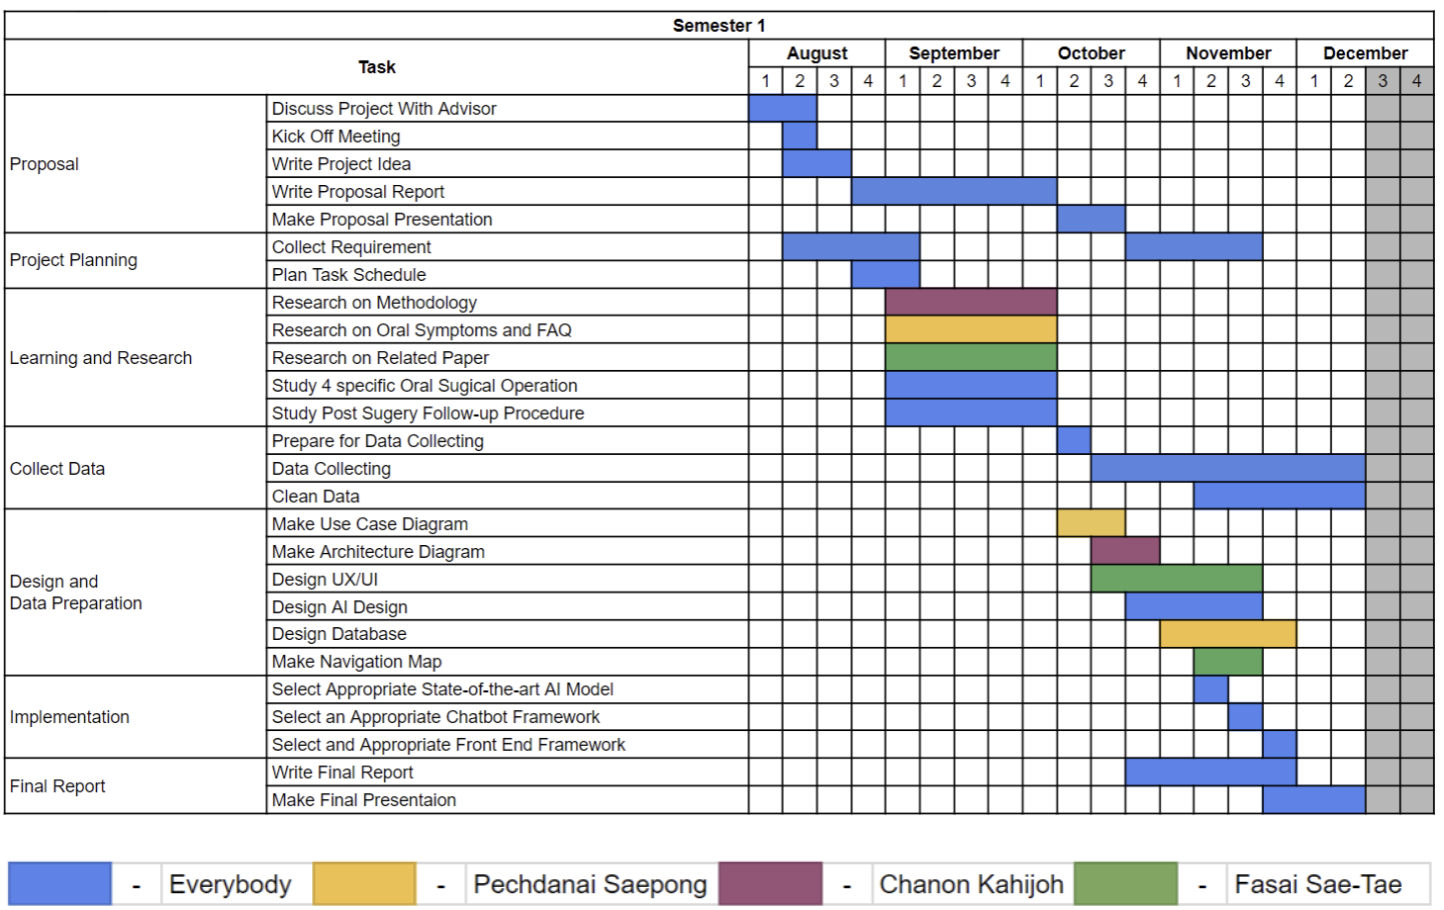
\includegraphics[width=.9\textwidth]{Image/Term1_Gantt.png}}
        \caption{Semester 1 plan schedule}\label{fig:Term1_Gantt}
      \end{figure}
      \begin{figure}[!h]
        \centering
        \fbox{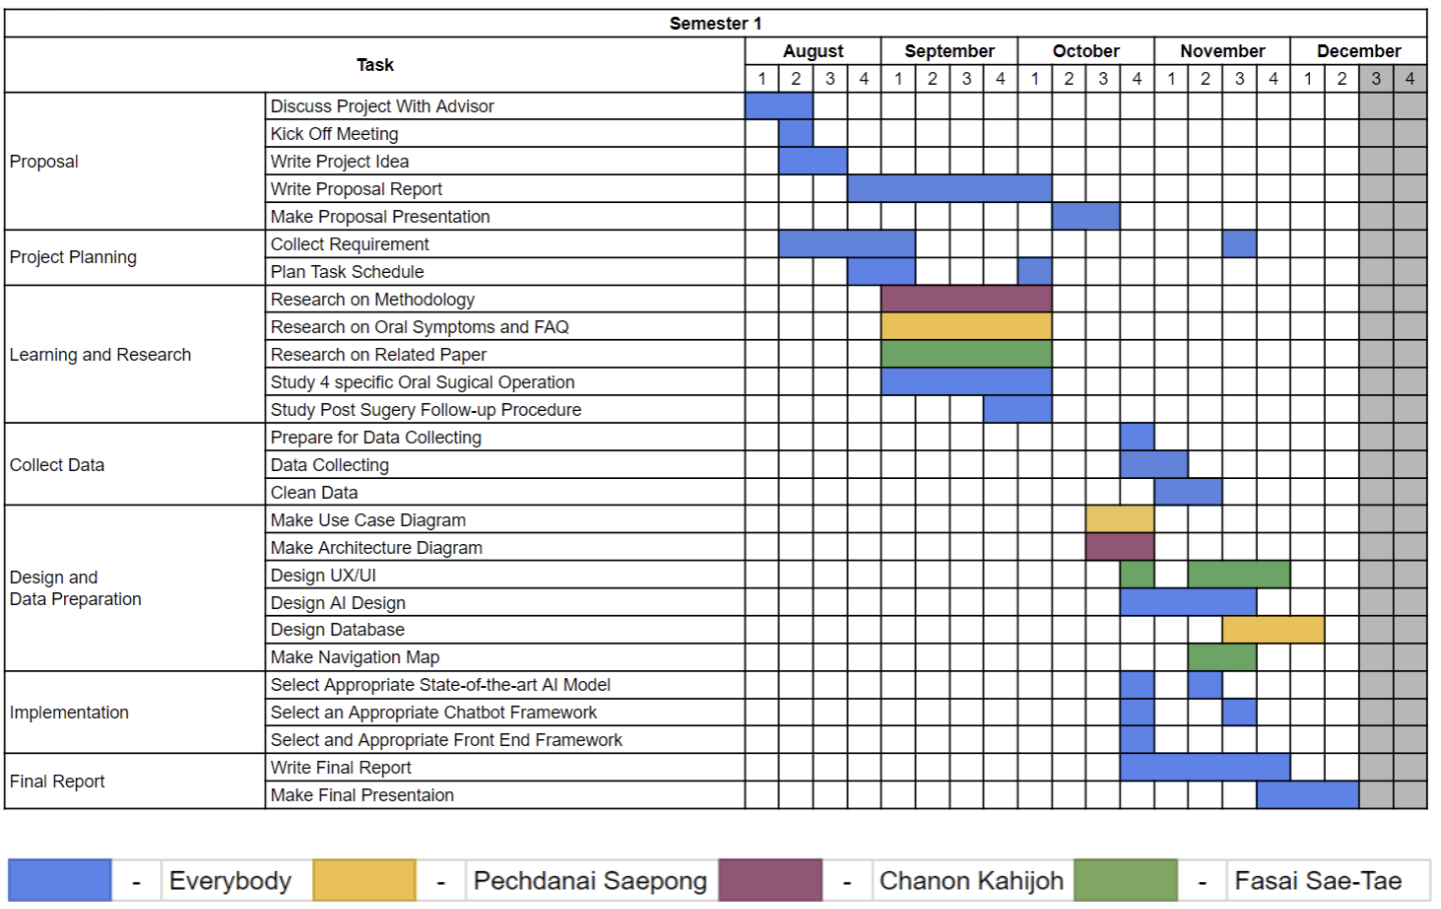
\includegraphics[width=.9\textwidth]{Image/Term1_Gantt_Actual.png}}
        \caption{Semester 1 actual schedule}\label{fig:Term1_Gantt_Actual}
      \end{figure}

    \subsection{Semester 2}
      \begin{enumerate}
        \item Deep Learning and Chatbot Implementation
          \begin{itemize}
            \item Model Implement
            \item Model Training
            \item Model Testing and Evaluation
          \end{itemize}
        \item Web Application Implementation
          \begin{itemize}
            \item Backend
            \item Frontend
            \item Test Case Design
            \item Unit Testing
            \item Usability Testing
          \end{itemize}
        \item Semester 2 Report
          \begin{itemize}
            \item Write Semester Report
            \item Semester Presentation
          \end{itemize}
      \end{enumerate}

    \subsection*{Deliverables for Term 2}
      \begin{itemize}
        \item Mobile application in both iOS and Android platform
        \item Testing result
        \item Feedbacks from users
        \item Senior Project Report
      \end{itemize}
      \begin{figure}[!h]
        \centering
        \fbox{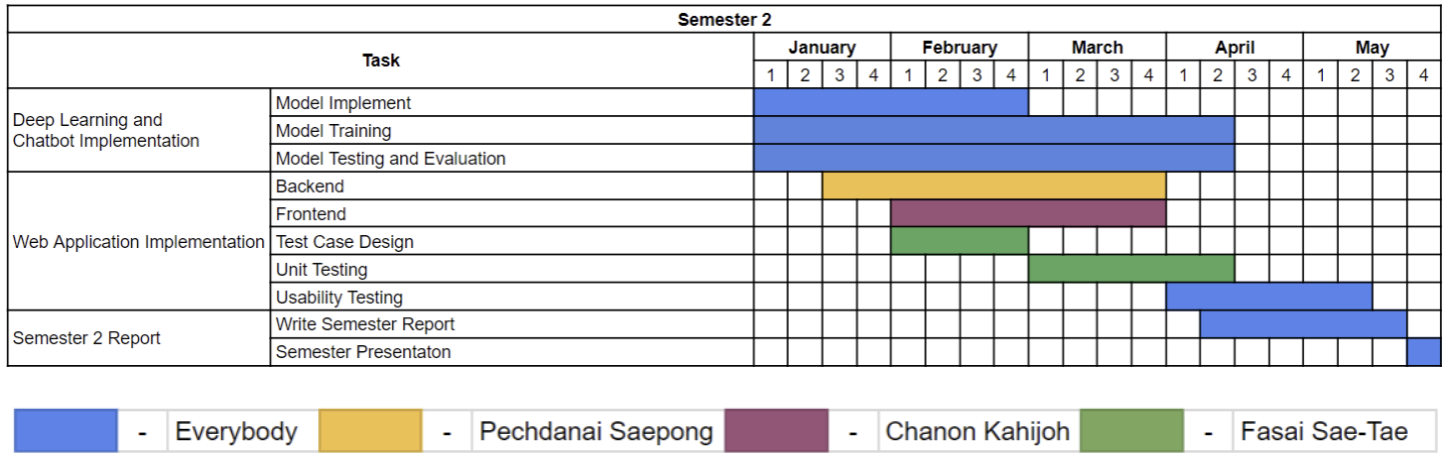
\includegraphics[width=.9\textwidth]{Image/Term2_Gantt.png}}
        \caption{Semester 2 plan schedule}\label{fig:Term2_Gantt}
      \end{figure}

\chapter{THEORY AND RELATED RESEARCH}
  \section{Introduction}
    \qquad This chapter will explain the details of the core concept and the solution planning. Theory and core concepts, languages and technologies, and related research will be discussed in this chapter. First, we will cover the theory and core concept of both dentistry and artificial intelligence. Second, programming languages and technologies that are intended to be used in this project will be described in the “Languages and Technologies” section. Lastly, related research and similar solution approaches to the objective will be discussed in the “Related Research and Competing Solutions” section.
    
  \section{Theory and Core Concepts}
    \qquad Common oral problems, including tooth decay, wisdom teeth complications, and gum disease, require consistent treatment for a considerable number of patients. Dentists, who routinely engage with patient inquiries and symptom tracking, have recommended that our focus be directed towards Tooth Extraction, Wisdom Tooth Removal, Periodontal Surgery, and Dental Implant Surgery. These specific procedures directly address the aforementioned common oral problems, aligning our work with the suggestions of dental professionals.\par
    \subsection{Tooth Extraction}
      \qquad Tooth extraction is a common dental procedure performed by a dentist or oral surgeon to remove a tooth from its socket in the jawbone. It is necessary for various reasons, including extensive tooth decay, crowding, tooth impaction, or as part of orthodontic treatment. Recovery typically takes a few days to a few weeks. The benefits of tooth extraction vary depending on the reason for the procedure. However, the disadvantages of tooth extraction often include challenges with chewing food and a potential loss of aesthetic appeal. Additionally, there may be complications that require careful monitoring, such as post-surgical swelling or infection.\par
    \subsection{Wisdom Tooth Removal}
      \qquad Wisdom tooth extraction, also known as third molar extraction, is a dental procedure performed to remove the third molars, commonly referred to as wisdom teeth. These teeth often become impacted or lead to various dental issues due to their slow growth and limited space in the jaw. Surgery becomes necessary for various reasons, including the prevention of pain arising from the inability of third molars to erupt properly or the prevention of issues related to crowded and misaligned teeth. However, the most common concerns associated with this procedure are the potential side effects after surgery, such as swelling, unusually significant or continuous discharge, or facial distortion lasting more than two weeks.\par
  
    \subsection{Periodontal Surgery}
      \qquad Periodontal surgery, also known as gum surgery, is a dental procedure aimed at treating various gum diseases and conditions. It involves the removal of infected gum tissue and, in some cases, the reshaping of the underlying bone to restore gum health and improve the stability of teeth. During this surgery, the dentist or periodontist carefully removes the diseased tissue and then shapes and contours the remaining gum and bone to promote optimal healing. In more advanced cases, bone grafts or tissue-stimulating proteins may be used to encourage tissue regeneration. Periodontal surgery is crucial in preventing the progression of gum diseases, reducing gum pockets, and ultimately preserving the natural teeth. Besides its significant impact on oral health, undergoing periodontal surgery can also enhance an individual's confidence and self-esteem by restoring a healthy, aesthetically pleasing smile.\par
  
    \subsection{Dental Implant Surgery}
      \qquad A dental implant is a technology used to replace missing teeth by employing sturdy materials as dental implants to serve as replacements for natural tooth roots. Presently, it is common to use dental implants that encompass both the root and the tooth, as they closely resemble natural teeth in appearance and function realistically. Additionally, they aid in preventing the deterioration of the jawbone where the implant is placed. To be a suitable candidate for dental implants, a patient must possess healthy gums and adequate bone support for the tooth roots. Following a root canal procedure, it is imperative for the patient to consistently maintain their oral health. Dental implants offer numerous advantages, including the prevention of teeth from shifting or becoming misaligned due to tooth loss, as well as contributing to the strengthening and preservation of oral hygiene.\par
  
  \section{Languages and Technologies}
    \subsection{Web Development Language}
      \subsubsection{JavaScript}
        \qquad JavaScript, abbreviated as JS and developed by Netscape in the mid-1990s, is one of the most used programming languages in web development. It enables the development of dynamic content within web pages, enhancing websites responsiveness to user interactions.\par
        \qquad Operating as a scripting language on the client side, JavaScript runs directly within web browsers, facilitating interaction with the Document Object Model (DOM), which represents a webpage's structure and content.\par
        \qquad JavaScript boasts a rich set of features and capabilities, including support for various data types, loops, functions, and more. Moreover, it offers many libraries and frameworks that simplify complex tasks.\par
        \qquad A key attribute of JavaScript is its capacity to handle asynchronous operations. Asynchronous operations enable data retrieval without disrupting the user’s experience, as these operations occur independently through mechanisms such as async/await and Promises.\par
      \subsubsection{TypeScript}
        \qquad Developed by Microsoft, TypeScript (or TS) is an enhanced version of JavaScript, adding strong typing and advanced features to the original language.\par
        \qquad One of the most noticeable changes from default JavaScript is the introduction of a strong tying system. TypeScript requires variables, function parameters, and function return types to be explicitly defined with data types. This enhances error detection during the development process, resulting in fewer bugs when the website is deployed. It also promotes easier cooperation between developers, as the code becomes more understandable.\par
        \qquad TypeScript offers additional features, such as interfaces and custom type definitions, which enable objects to have specific shapes. This feature enhances code comprehension and facilitates integration with third-party libraries.\par
      
      \subsubsection{Python}
        \qquad Python, famous for its ease of use and readability, has gained in popularity in web programming due to its flexibility and an extensive collection of frameworks designed for web application development. It is frequently employed in web backend development, offering developers a wide range of frameworks and libraries to choose from. This diversity makes it an attractive choice for creating robust and scalable websites.\par
  
      \subsubsection{Hypertext Markup Language}
        \qquad Hypertext Markup Language, abbreviated as HTML, serves as the standard language for creating the structural framework of websites. It uses a markup syntax consisting of tags to define various components, including headings, paragraphs, links, images, etc. HTML’s simplicity, adaptability, and compatibility with multimedia features have solidified its enduring importance in the realm of website development. It stands as an indispensable tool for developing everything from straightforward web pages to complex websites.\par
  
      \subsubsection{Cascading Style Sheet}
        \qquad Cascading Style Sheets, abbreviated as CSS, is commonly referred to as a "style sheet." It is a language used to format HTML documents, with CSS being responsible for defining rules that specify the presentation of content within a document. These rules encompass aspects such as text color, background color, font type, and text positioning. The fundamental concept behind CSS is the separation of HTML document content from the instruction used for formatting its display. By employing this separation, CSS achieves two primary objectives. Firstly, it ensures that the document's display format is independent of its content, facilitating the task of formatting HTML documents, especially when the content undergoes frequent changes. Secondly, CSS enables precise control over the presentation format of HTML documents, ensuring consistency across all pages within the same website. Styling rules for HTML documents were initially introduced in HTML 4.0 back in 1996, in the form of CSS Level 1 recommendations established by the World Wide Web Consortium (W3C).\par
    
    \subsection{Front-end Framework}
      \qquad Front-end frameworks play a crucial role in web development by simplifying the creation of user interfaces. They encompass design, layout, and interactive elements such as forms and buttons. These frameworks provide pre-written code that includes HTML, CSS, and JavaScript components, facilitating code reuse and maintaining consistency across web projects. By leveraging front-end frameworks, developers can efficiently generate HTML and CSS, design responsive layouts for various devices, ensure a consistent user experience, automate repetitive tasks, and manage their code efficiently. Ultimately, front-end frameworks streamline and structure the development process, enabling the creation of user-friendly and visually appealing web applications. Examples of front-end frameworks are as follows:\par
      \begin{itemize}
        \item React: A front-end framework, React stands apart because of its virtual Document Object Model (DOM), which enhances its functionality. It is a perfect framework for those who expect high traffic and require a steady platform to manage it. 
        \item Angular: Formally released in 2016, the Angular framework was established by Google to bridge the gap between the mounting demands of technology and conventional notions that displayed the results. In contrast to React, Angular is distinctive with its two-way data binding trait. It means that there is real-time synchronization between the view and model, where any alteration in the model replicates promptly on the view and vice versa.To reduce doctors and staff by minimizing repeated questions and explanations from patients.
        \item Vue.js: It has a small size and offers two main benefits – a visual DOM and a component-based structure. It also employs two-way data binding. This front-end framework is versatile and assists with various tasks when building web applications. The difference between Vue and React is that Vue is a JS framework while React is a JS library. So, Vue is more suitable for large projects.
        \item Semantic-UI: The objective of Semantic lies in empowering the designers and developers by creating a language for sharing UI. It uses natural language that makes the entire code self-explanatory. The framework is comparatively new to the ecosystem. Still, with its striking user interface, simple functionalities, and features, it has become one of the most popular front-end frameworks.
        \item Next.js: Used by some of the world's largest companies, Next.js enables you to create full-stack web applications by extending the latest React features and integrating powerful Rust-based JavaScript tooling for the fastest builds.
      \end{itemize}
  
    \subsection{Backend Framework}
      \qquad A backend framework serves as a foundational platform for developers to expedite the creation of web and mobile applications with standardization. In the context of backend frameworks, they simplify server-side development by offering tools, libraries, and components that streamline the construction of web applications. These frameworks automate various aspects of web development, enhancing efficiency and cleanliness in code design. Examples of backend frameworks are as follows:\par
      \begin{itemize}
        \item ExpressJS: It is a minimal Node.js framework used to develop highly flexible applications.
        \item Django: Django is the most popular Python framework used in web development. Based on the Don’t Repeat Yourself (DRY) principle, Django focuses on code reusing, thus enhancing the development speed. It is also a very secure framework.
        \item Node.js: JavaScript is the most popular programming language in the world. With the emergence of Node.js, JavaScript’s popularity in the backend development community increased rapidly, and in the last decade, Node.js has become one of the top names.
        \item Flask: It’s a simple, highly flexible, and performing web framework. Being a lightweight framework, or micro-framework, it is easy to learn and understand Flask. Moreover, being a Python framework, it is very user-friendly.
      \end{itemize}
    
    \subsection{Chatbot}
      \qquad A chatbot is a machine learning (ML) or artificial intelligence (AI) system designed to simulate and handle human conversations, whether written or spoken. These AIs enable users to interact with digital devices as if they were having a conversation with a human. Chatbots can vary widely in complexity, from basic systems that respond to user queries to advanced digital assistants that learn and adapt over time, providing personalized experiences as they collect and process data.\par
      \subsubsection{Chatbot Framework}
        \qquad A Bot Framework is a platform where developers create and define the behavior of chatbots. It simplifies the complex task of building chatbots that can operate on various messaging platforms and software development kits (SDKs). While some frameworks claim “write once, deploy anywhere" capabilities, in practice, developers often need to create separate chatbots for each messaging platform. The Bot Framework comprises components such as the Bot Builder SDK, Bot Connector, Developer Portal, Bot Directory, and an emulator for testing. However, it may not be the best choice for beginners looking to learn chatbot development due to its complexity.\par
        \qquad Examples of Bot frameworks include:\par
        \begin{itemize}
          \item DialogFlow
          \item Microsoft Bot Framework
          \item Rasa
          \item Amazon Lex
          \item IBM Watson Assistant
          \item Wit.ai
          \item Botpress
        \end{itemize}
      
      \subsubsection{Pretrained Chatbot Model}
        \qquad A pretrained chatbot model is a Natural Language Processing (NLP) model that has been trained on a wide range of text data from sources such as books, articles, social media, etc. These models are equipped with the capability to understand and generate text that closely resembles human language, making them valuable for chatbot development and other natural language tasks. These chatbots can also undergo fine-tuning or additional training for a specific task or domain to enhance their accuracy and performance.\par
        \paragraph{DeBERTa}\mbox{}\\
          \null\qquad DeBERTa (Decoding-enhanced BERT with disentangled attention) is a neural language model architecture designed to enhance the performance of pre-trained models like BERT (Bidirectional Encoder Representations from Transformers) and RoBERTa (Robustly optimized BERT approach) with two techniques, a disentangled attention mechanism and an enhanced mask decoder.\par
          \qquad The disentangled attention mechanism involves representing each word with two vectors—one for content and one for position. Attention weights among words are then calculated using disentangled matrices for content and relative positions, allowing the model to independently consider semantic content and positional relationships during computations.\par
          \qquad The enhanced mask decoder replaces the output softmax layer to predict masked tokens during model pre-training. Additionally, a new virtual adversarial training method is applied during fine-tuning to enhance the model's generalization for downstream tasks.\par
          \qquad The DeBERTa V2 model is a variant of the transformer architecture designed for question-answering tasks. Its structure consists of an embedding layer for word representations, employing layer normalization and dropout for regularization. The core encoder is composed of multiple DeBERTa V2 layers, each featuring a disentangled self-attention mechanism, an intermediate layer with GELU activation, and output layers for attention and transformation. The model incorporates relative positional embeddings to efficiently capture token dependencies. The final layer includes a linear output module specialized for predicting start and end positions in the input sequence, crucial for question answering. Overall, DeBERTa V2 integrates advanced attention mechanisms and positional embeddings to enhance its ability to capture complex relationships within the input data for improved performance in question-answering tasks.\par
  
        \paragraph{mDeBERTa}\mbox{}\\
          \null\qquad mDeBERTa is the multilingual version of DeBERTa. Both models have the same architecture but mDeBERTa supports multiple languages while DeBERTa supports only English.\par
      
    \subsection{Machine Learning}
      \qquad Machine Learning (ML) is a branch of Artificial Intelligence that tries to replicate how humans work. It uses the accumulated data in order to let machines learn step by step in order to improve its accuracy in the task they are trained to do.\par
        
        \subsubsection{Decision Tree}
          \qquad A decision tree is a supervised machine learning algorithm used for categorizing and regression tasks. A decision tree consists of root node, decision nodes, leaf nodes, splitting, pruning, and branches.\par
          \qquad The decision tree operates by employing various algorithms to decide to split a node into two or more sub-nodes. Decision trees work by iteratively partitioning nodes based on all available features and subsequently selecting the split that leads to the most uniform or homogeneous sub-nodes in terms of the target variable. This aims to create clear and distinct decision boundaries within the dataset, facilitating more accurate predictions or classifications by the decision tree model.\par
          \begin{figure}[!h]
            \centering
            \fbox{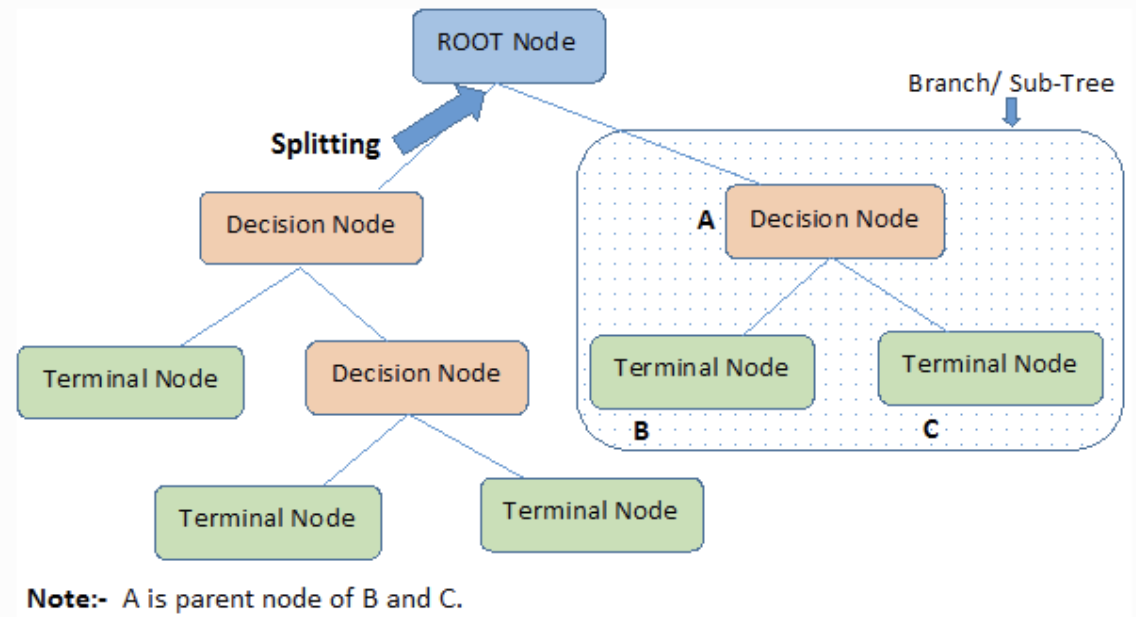
\includegraphics[width=.6\textwidth]{Image/Decision_Tree.png}}
            \caption{Diagram explaining Decision Tree}\label{fig:Decision_Tree}
          \end{figure}
        
        \subsubsection{Random Forest}
          \qquad Random Forest is the combination of many decision trees and using results from all decision trees by either averaging or majority voting making it less biased which helps in overfitting problems. As you can see from Figure 1.2, the final results are obtained after getting results from many decision trees.\par
          \begin{figure}[!h]
            \centering
            \fbox{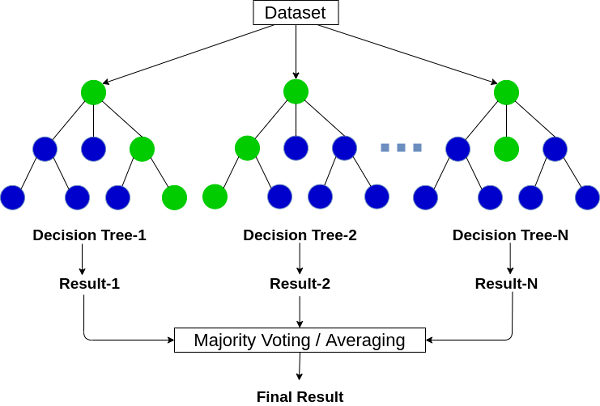
\includegraphics[width=.6\textwidth]{Image/Random_Forest.png}}
            \caption{Diagram explaining Random Forest}\label{fig:Random_Forest}
          \end{figure}
    \subsection{Augmenting Data}
      \qquad We augmented text data to expand data while trying to simulate human error such as misspelling a word or typing a key by mistake. We can achieve this by inserting random characters into the questions, deleting random characters in the questions, and swapping random characters in the questions. We are also able to expand by paraphrasing the sentence. In order to have the best performance for paraphrasing we need to first translate it to English then let the AI model paraphrase as it is an English paraphrasing model then translate the results back to Thai.\par
    \subsection{Proposed Framework}
      \qquad The proposed framework has 2 components that are to be used together:\par
      \begin{itemize}
        \item Random Forest: classify the input question into class
        \item BERT: answer the user's question based on the identified class
      \end{itemize}
      \qquad We first input a question into a random forest in order to classify which class it belongs to. We then input that class in order to use the correct context in order to get the correct answer. With this method we can reduce time taken while trying to increase its accuracy\par
  \section{Related research / Competing solutions}
    \subsection{Related Research}
      \qquad \textbf{Designing a Competent Chatbot to Counter the COVID-19 Pandemic and Empower Risk Communication in an Emergency Response System}\par
      \begin{figure}[!h]
        \centering
        \fbox{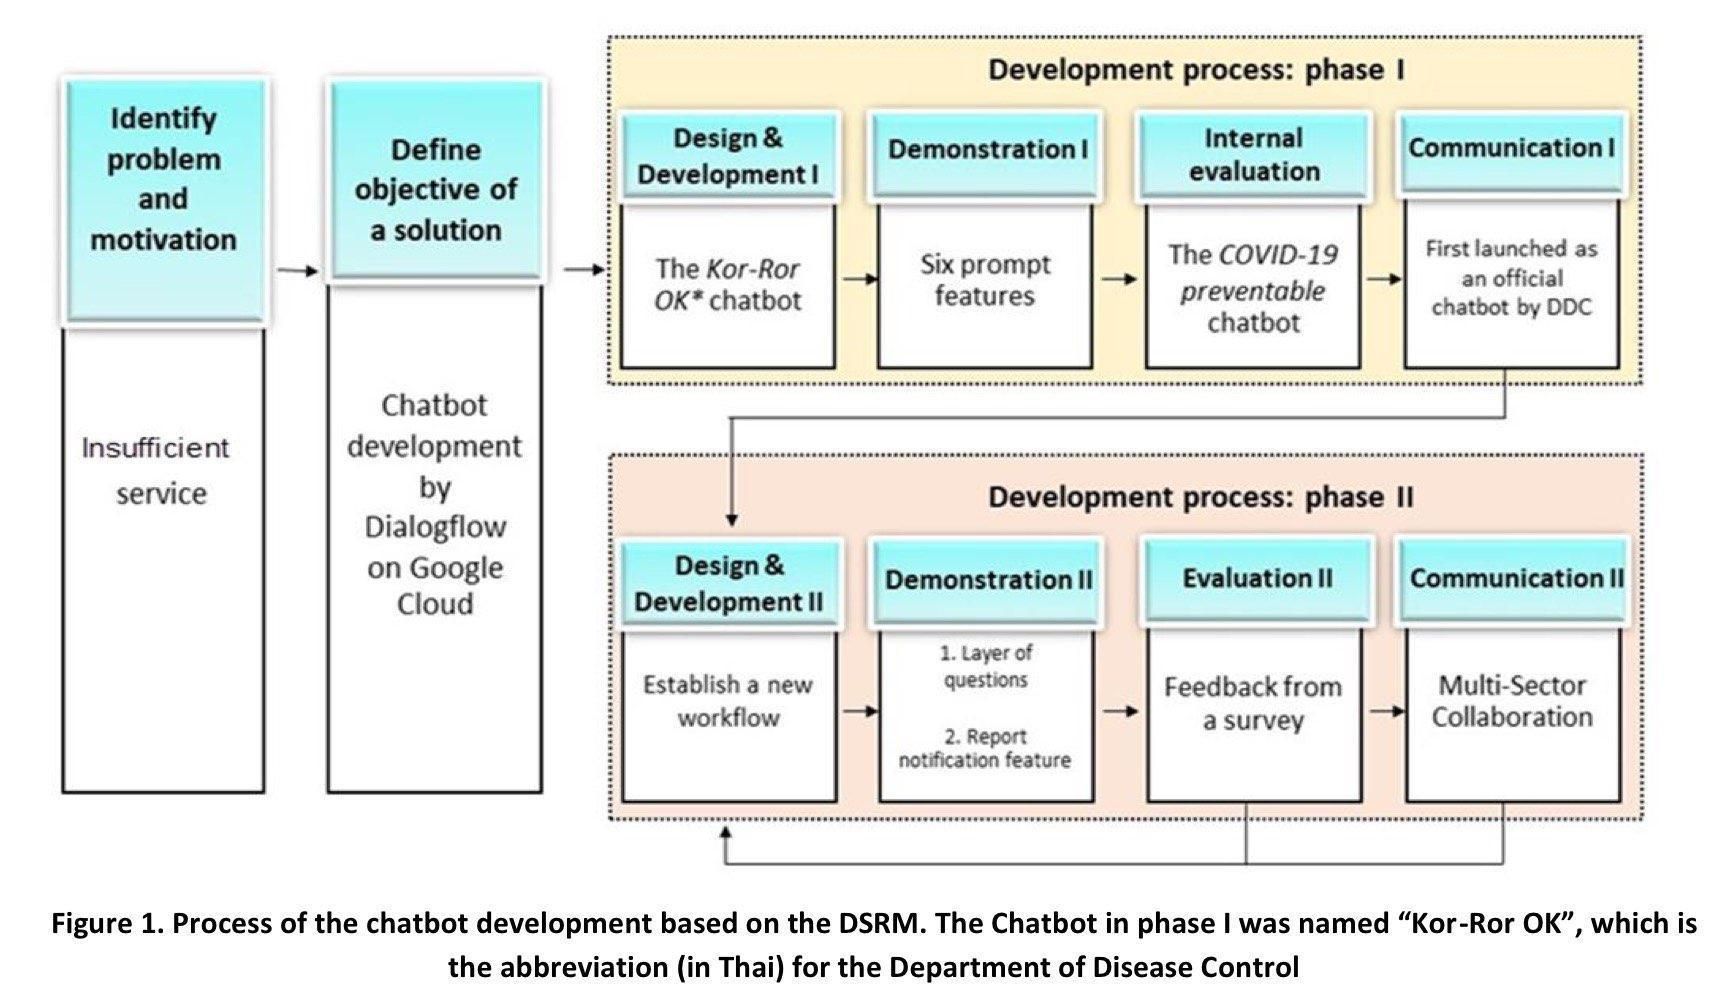
\includegraphics[width=.6\textwidth]{Image/Research_1.jpg}}
        \caption{Overview of DSRM development process}\label{fig:Research_1}
      \end{figure}
      \qquad This paper presented the development process and the characteristics of a competent chatbot, with an emphasis on COVID-19. The paper used Design Science Research Methodology (DSRM) as the development process to implement the chatbot, which consisted of 6 steps. Line Application was chosen as the main channel for the development and was deployed using Dialog Flow. In phase one, the development focused on implementing a chatbot capable of answering various frequently asked questions and providing knowledge about COVID-19. The emphasis shifted to more complex questions and chatbot efficiency in phase 2 of the development.\par
      \qquad The knowledge in this paper regarding the development process can be used and applied to our development process since the output products are similar in terms of use. However, the step of product evaluation will be different since we do not have a large number of users, and some key features, such as follow-up, are different.\par
    \subsection{Competing Solution}
      \subsubsection{DentalChat}
        \begin{figure}[!h]
          \centering
          \fbox{
\includegraphics[width=.2\textwidth]{Image/DentalChat_Logo.png}}
          \caption{DentalChat Logo}\label{fig:DentalChat_Logo}
        \end{figure}
        \qquad DentalChat is an AI dental care application that connects and allows users to ask dental questions and is assisted by a dentist in real-time. DentalChat features consist of finding a local dentist, asking dental questions, post consult requests, and chatting with the dentist.\par
      \subsubsection{PsyJai}
        \begin{figure}[!h]
          \centering
          \fbox{
\includegraphics[width=.2\textwidth]{Image/PsyJai_Logo.png}}
          \caption{PsyJai Logo}\label{fig:PsyJai_Logo}
        \end{figure}
        \qquad PsyJai is a comprehensive automated AI mental health assistance system collaboration that can perform mental health assessments and provide psychological care based on the principles of psychology. PsyJai provides services through Facebook and Line. PsyJai has 4 main features: 1. Emotional Status Screening 2. Basic Care with Psychological Principles 3. General Conversations 4. Mood Dashboard.\par
      \subsection{Comparison Table}
        \begin{table}[h]
          \centering
          \caption{\centering Comparison table between our proposed solution, DentalChat and PsyJai}\label{tab:Comparison_Table}
          \begin{tabular}{|c|c|c|c|} \hline
            & Our proposed Solution & DentalChat & PsyJai \\\hline
            Symptom Diagnosis & AI System & Manual & AI System \\\hline
            Post-Surgery Follow Up & AI System & - & - \\\hline
          \end{tabular}
        \end{table}
        \qquad According to Table 1, our proposed solution has 2 main features: symptom diagnosis and post-surgery follow-up, both of which are AI-based systems. In contrast, DentalChat only has a symptom diagnosis feature, which is manually answered by the doctors. Psyjai also has an AI-based system for symptom diagnosis but does not have the post-surgery follow-up feature.\par

\chapter{DESIGN AND METHODOLOGY}
  \section{Introduction}
  \qquad This chapter will discuss the features and architecture including the features, functionalities, designing method and diagram of the web application. We will be discussing in detail about the functionality and the architecture of the web. \par
  \section{Project Functionality}
    \subsection{System Requirements}
    \begin{itemize}
      \item The web application must allow user to login via Line Account.
      \item The web application must automatically login if user access via line.
      \item The web application must allow all users to ask frequently asked questions from chatbot.
      \item The web application must allow the login users to scan qr code to create a new follow-up case.
      \item The web application must allow login users to answer follow-up chatbot.
      \item The web application must allow login users to view their own profile.
      \item The web applications must allow all login users to logout.
    \end{itemize}

    \subsection{Feature List}
      \subsubsection{Patient Registration}
      \qquad This feature is designed as user registration for the web application, and can be accessible through Line Official. When the user accesses the web application via Line Official for the first time, they need to authorize the linking to their Line account. Once the user has authorized, when accessing the web application through Line Official menu, the user will be automatically logged in. \par
      \subsubsection{Frequently Asked Questions answering Chatbot}
      \qquad This feature is designed to provide information and answer common questions about specific surgical procedures, including Tooth Extraction, Wisdom Tooth Removal, Periodontal Surgery, and Dental Implant Surgery. Users can input their question related to the surgery mentioned, and the chatbot will provide the relevant information. When there are questions that the chatbot has never encountered and cannot answer, the chatbot will return an error message and will keep that question for future training. \par
      \subsubsection{Follow-up Chatbot}
      \qquad This feature is designed to streamline the post-surgery monitoring process by replacing the traditional method of medical staff making follow-up calls to check on patients' conditions. The chatbot is proactive in questioning by targeting follow-up questions based on the surgery the patient has undergone to gather an insight of the patient's current state to assess their condition and to provide appropriate advice. \par
      \subsubsection{Add new follow-up case}
      \qquad This feature is to create a new follow-up case by enabling the user to generate a follow-up chatbot by scanning a given QR code at the healthcare unit and selecting the operation that has undergone. \par
      \subsubsection{View past follow up case}
      \qquad This feature allows the user to view their past follow-up case history. 
  \section{System Architecture}
  \begin{figure}[!h]
    \centering
    \fbox{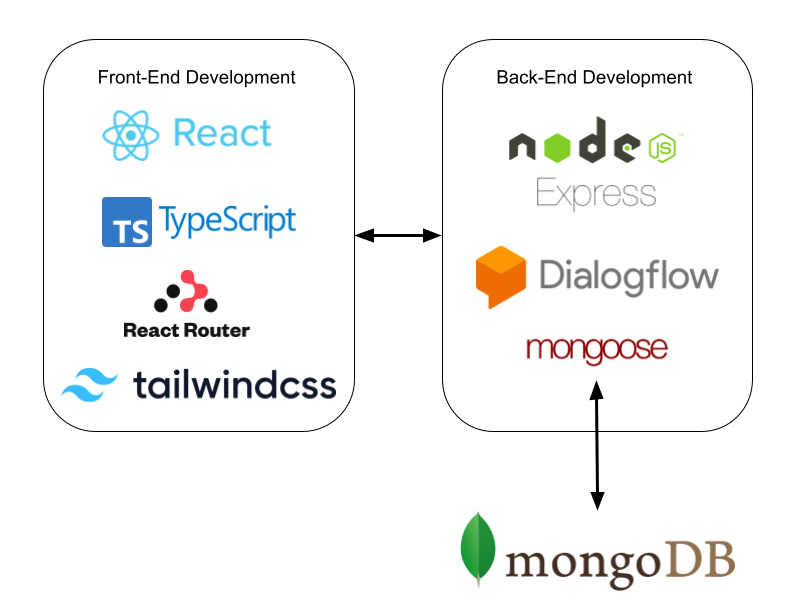
\includegraphics[width=.8\textwidth]{Image/System_Architecture.png}}
    \caption{Architecture Diagram}\label{fig:System_Architecture}
    \begin{flushleft}
      \qquad In the Figure 3.1 above, show the architecture design of our project. The Technology that we use in this project include. \par
      \begin{itemize}
        \item[] 1. React (Front-end JavaScript library for building UI)
        \item[] 2. Sweetalert2 (beautiful popup box react component use in React)
        \item[] 3. TailwindCSS (Css framework for styling the UI and use with React)
        \item[] 4. Chart.js (free open source JavaScript library for data visualization)
        \item[] 5. Node.js (back-end JavaScript runtime environment)
        \item[] 6. Express (Back-end framework for Node.js for building REST API)
        \item[] 7. MongoDB (NoSQL Database)
        \item[] 8. Mongoose (Node.js based Object Data Modelling (ODM) library for MongoDB)
        \item[] 9. React selects a flexible and beautiful Select Input control for ReactJS with multiselect, autocomplete, async and creatable support
        \item[] 10. Dialogflow is used for follow-up using its api in order to reduce resource used in client browser
      \end{itemize}
    \end{flushleft}        
  \end{figure}

  \newpage
  \section{Use Case Diagram}
  \begin{figure}[!h]
    \centering
    \fbox{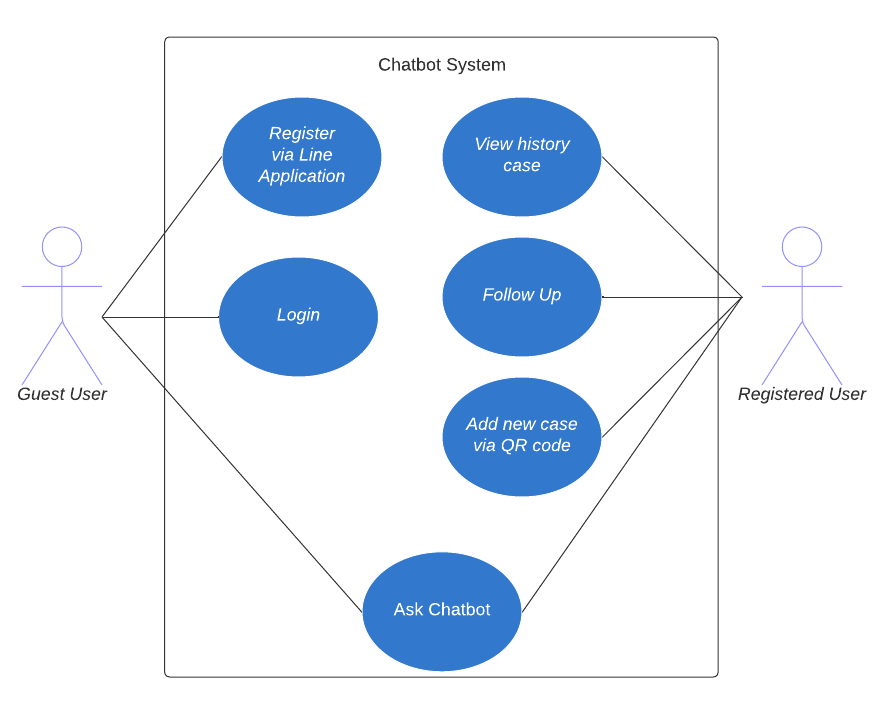
\includegraphics[width=.99\textwidth]{Image/Use_Case.png}}
    \caption{Use Case Diagram}\label{fig:Use_Case}
  \end{figure}

  \section{Use Case Narrative}
    \subsection{Question Answer}
      \qquad Use case name: Question Answer \par
      \qquad Actors: All User \par
      \qquad Goal: User ask questions and receive answer \par
      \qquad Preconditions: - \par
      \qquad Main success scenario:
      \begin{itemize}
        \item[] 1. User go to home page
        \item[] 2. User select chatbot button
        \item[] 3. User Input question
        \item[] 4. System answer the question
      \end{itemize}

    \subsection{Login}
      \qquad Use case name: Login \par
      \qquad Actors: General User \par
      \qquad Goal: User login to the system \par
      \qquad Preconditions: User already registered \par
      \qquad Main success scenario:
      \begin{itemize}
        \item[] 1. User go to website homepage
        \item[] 2. User select login with line application button
        \item[] 3. System navigate to line page and set token to this account
        \item[] 4. System navigate user to FAQ page
      \end{itemize}

      \subsection{Register}
        \qquad Use case name: Register \par
        \qquad Actors: General User \par
        \qquad Goal: Add new user to the system \par
        \qquad Preconditions: - \par
        \qquad Main success scenario:
        \begin{itemize}
          \item[] 1. User go to website homepage
          \item[] 2. User select login with line button
          \item[] 3. System navigate to line official login page
          \item[] 4. User select allow button
          \item[] 5. System get new user
        \end{itemize}
        \qquad Extension (a)
        \begin{itemize}
          \item[] 1a. User open line application
          \item[] 2a. User scan qr code
          \item[] 3a. User add line official
          \item[] 4a. User select allow button
          \item[] 5a. System get new user
        \end{itemize}
      
      \subsection{Follow-up}
        \qquad Use case name: Follow up \par
        \qquad Actors: Registered User (Patient) \par
        \qquad Goal: Registered User answer follow up question then system send suggestion \par
        \qquad Preconditions: User have done surgery and scan the QR code \par
        \qquad Main success scenario:
        \begin{itemize}
          \item[] 1. User login to the system
          \item[] 2. System ask follow-up question
          \item[] 3. Login user answer the question
          \item[] 4. The answer relate to the question
          \item[] 5. System analysis and give suggestion to patient
        \end{itemize}
        \qquad Extension (a)
        \begin{itemize}
          \item[] 4a. The answer does not relate to the question.
          \item[] 5a. System sends an error message. Return to step2.
        \end{itemize}

      \subsection{View case history}
        \qquad Use case name: View case history \par
        \qquad Actors: Registered User (Patient) \par
        \qquad Goal: Registered User (Patient) access user case page \par
        \qquad Preconditions: User have done surgery \par
        \qquad Main success scenario:
        \begin{itemize}
          \item[] 1. User login to the system
          \item[] 2. System navigate to FAQ Page
          \item[] 3. User select “Profile” button
          \item[] 4. User access to Profile Page with case history
        \end{itemize}
      \subsection{Add new case via QR code}
        \qquad Use case name: Add new case via QR code \par
        \qquad Actors: Registered User (Patient) \par
        \qquad Goal: Registered User (Patient) add new case to system \par
        \qquad Preconditions: User have done surgery \par
        \qquad Main success scenario:
        \begin{itemize}
          \item[] 1. User login to the system
          \item[] 2. User select scan qr code in system line official
          \item[] 3. User scan qr code
          \item[] 4. User access to the form
          \item[] 5. User select 1 treatment operation
          \item[] 6. User submit the form to system
        \end{itemize}

\newpage
    \section{Activity Diagram}
      \subsection{Question Answering}
      \begin{figure}[!h]
        \centering
        \fbox{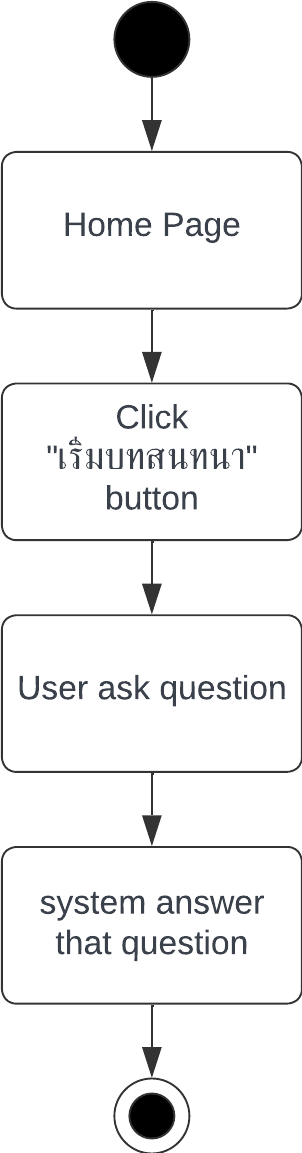
\includegraphics[width=.15\textwidth]{Image/AD_FAQ.png}}
        \caption{Question Answering Activity Diagram}\label{fig:AD_FAQ}
        \begin{flushleft}
          \qquad When user access to homepage and click “\textthai{เริ่มบทสนทนา}” button, system will show chatbot interface and user can input a question in input text box then system will answer that question. \par
        \end{flushleft}
      \end{figure}

      \subsection{Login}
      \begin{figure}[!h]
        \centering
        \fbox{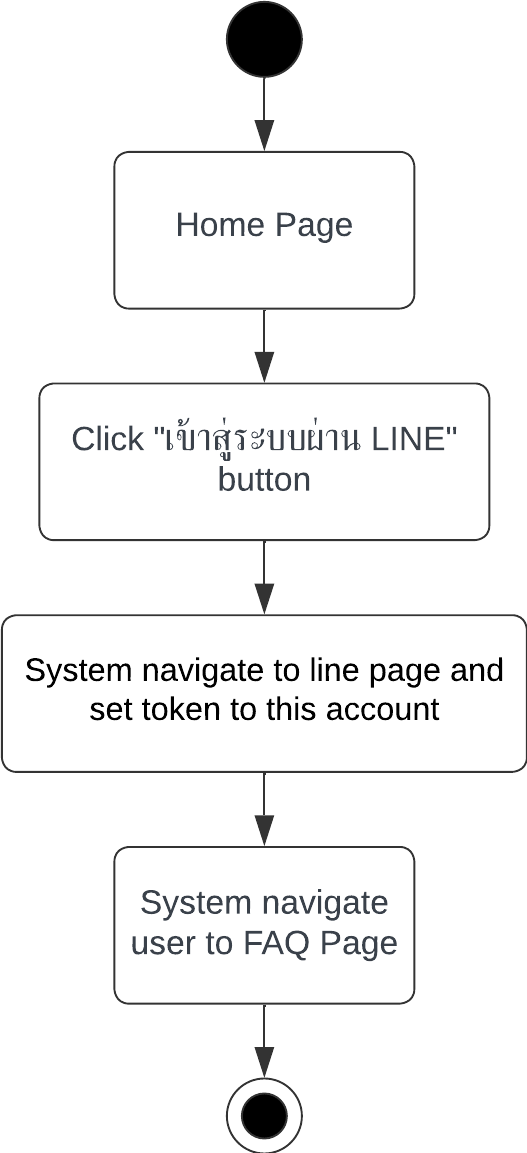
\includegraphics[width=.15\textwidth]{Image/AD_Login.png}}
        \caption{Login Activity Diagram}\label{fig:AD_Login}
        \begin{flushleft}
          \qquad When user access to homepage and click “\textthai{เข้าสู่ระบบผ่าน} LINE”, system will navigate user to line page then navigate to FAQ page. \par
        \end{flushleft}
      \end{figure}
\newpage
      \subsection{Register}
      \begin{figure}[!h]
        \centering
        \fbox{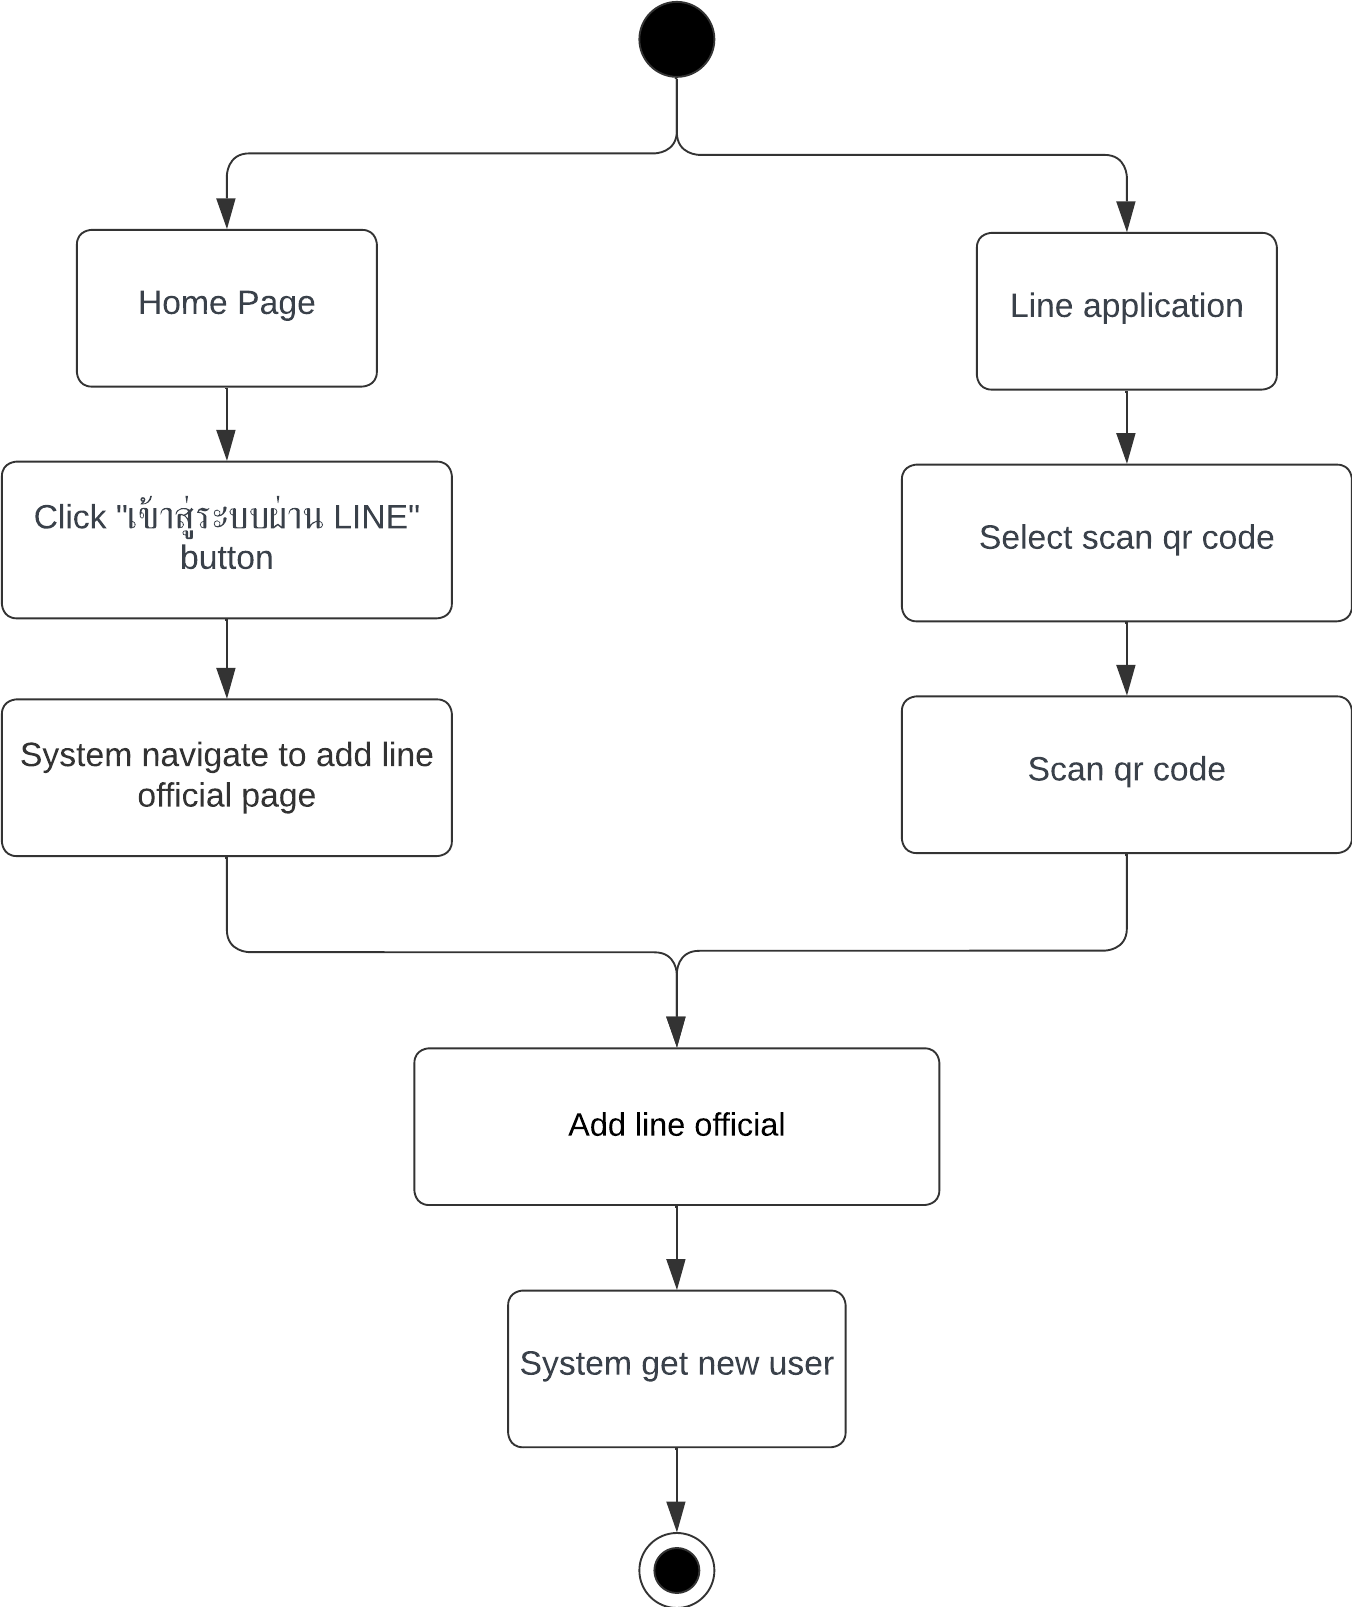
\includegraphics[width=.4\textwidth]{Image/AD_Regis.png}}
        \caption{Register Activity Diagram}\label{fig:AD_Register}
        \begin{flushleft}
          \qquad When user access to homepage and click “\textthai{เข้าสู่ระบบผ่าน} LINE” button, system will navigate user to add line official page and user click add line official then system will register this user automatically. In another way, user access via line application and select scan qr code then scan our qr code at medical unit, and select add line official, system will register this user automatically as well. \par
        \end{flushleft}
      \end{figure}

      \subsection{Follow-Up}
      \begin{figure}[!h]
        \centering
        \fbox{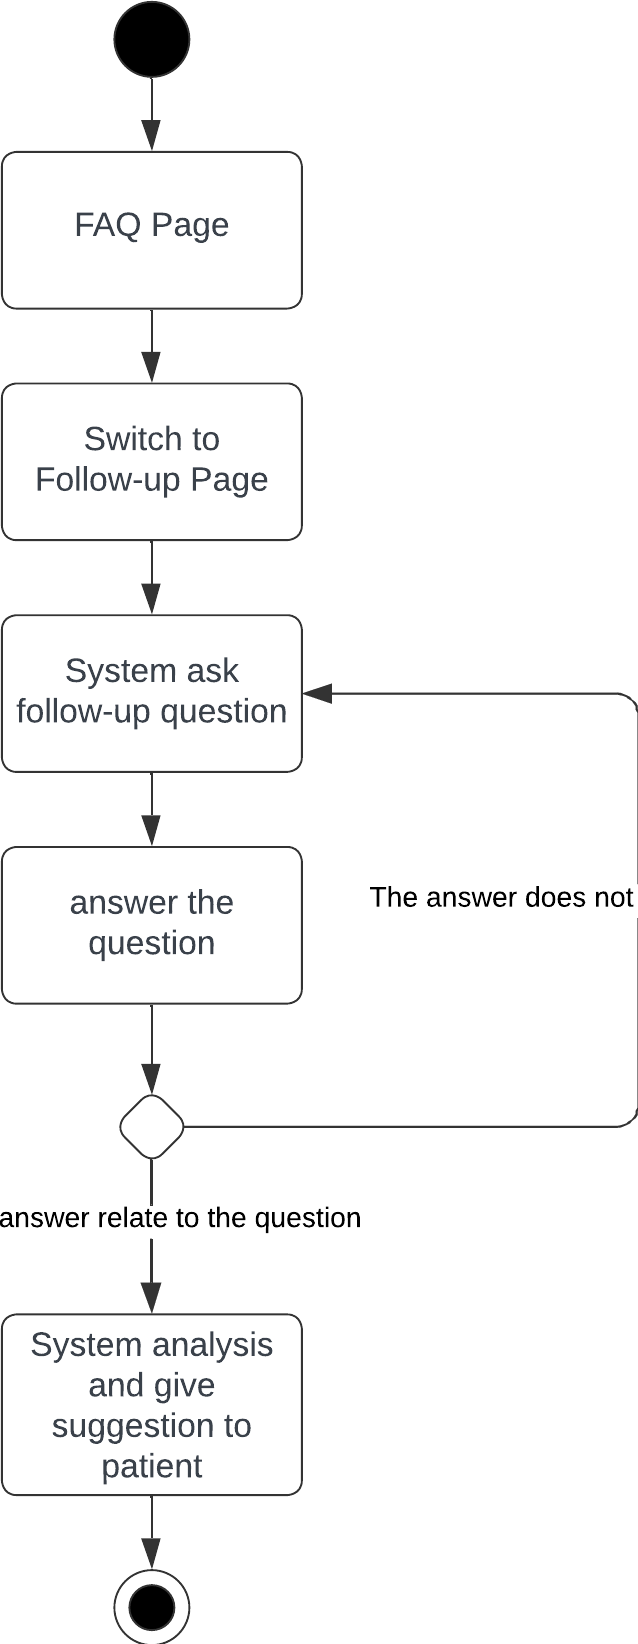
\includegraphics[width=.15\textwidth]{Image/AD_Follow.png}}
        \caption{Follow-Up Activity Diagram}\label{fig:AD_Follow}
        \begin{flushleft}
          \qquad When user access FAQ page after login completely and switch to Follow-up page, system will show follow-up chatbot interface then system will ask follow-up question, and user answer questions, if answer related to question system will analyze that answer and give suggestion to user, but if answer does not related to question, system will try to ask again to get related answer from user.  \par
        \end{flushleft}
      \end{figure}
\newpage
      \subsection{View case history}
      \begin{figure}[!h]
        \centering
        \fbox{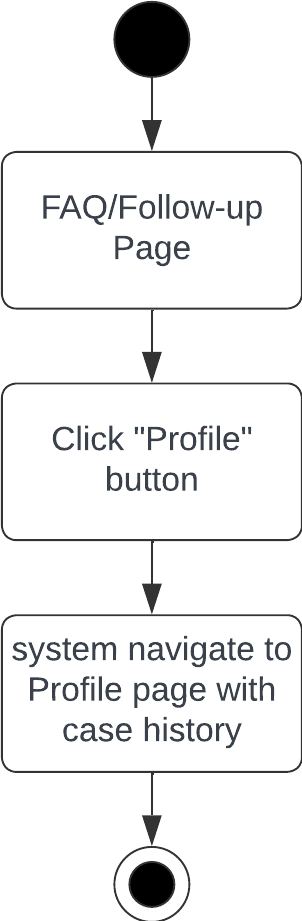
\includegraphics[width=.15\textwidth]{Image/AD_ViewCase.png}}
        \caption{View case history Activity Diagram}\label{fig:AD_ViewCase}
        \begin{flushleft}
          \qquad When user access FAQ or Follow-up page and click on “Profile” button, system will navigate to profile page with case history.  \par
        \end{flushleft}
      \end{figure}
      \subsection{Add new case via QR code}
      \begin{figure}[!h]
        \centering
        \fbox{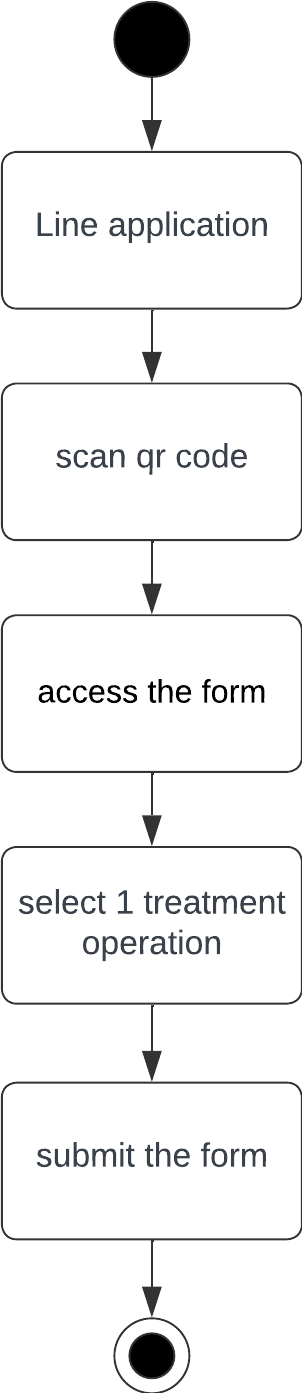
\includegraphics[width=.12\textwidth]{Image/AD_AddCase.png}}
        \caption{Add new case via QR code Activity Diagram}\label{fig:AD_AddCase}
        \begin{flushleft}
          \qquad When user open line application and scan our qr code, user will access to the form that user need to select one of treatment operations and submit the form.  \par
        \end{flushleft}
      \end{figure}

  \section{Navigation Map}
    \begin{figure}[!h]
      \centering
      \fbox{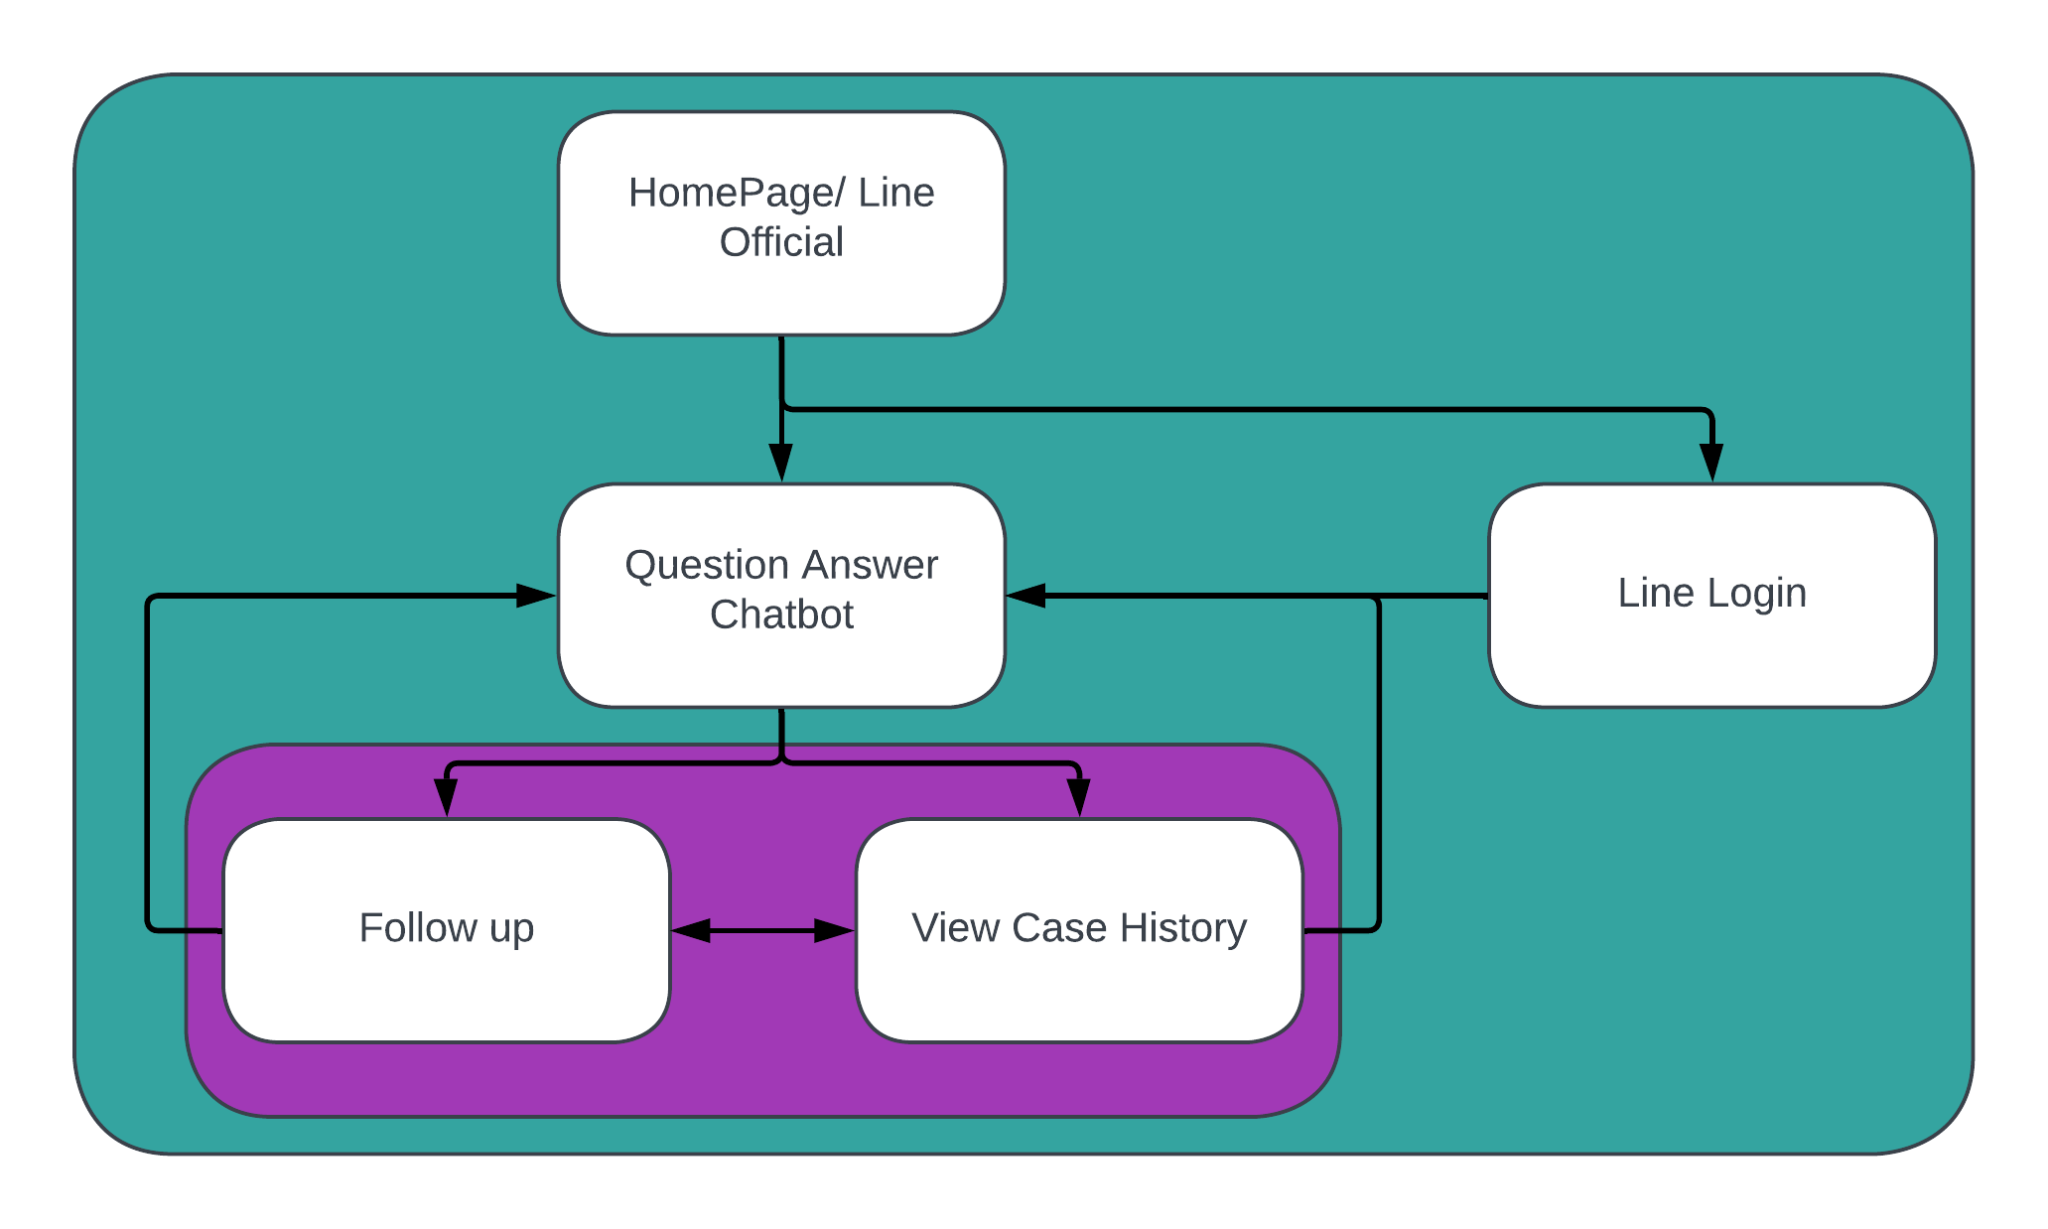
\includegraphics[width=.6\textwidth]{Image/Navigation_Map.png}}
      \caption{Chatbot web application navigation map}\label{fig:Navigation_Map}
      \begin{flushleft}
        \qquad For the web application, there are two roles which are Guest user and Registered user. Every user starts with the Homepage, Guest can only access the FAQ Chatbot and Login page, while Registered users can also access the Follow Up page and View Case History page. \par
        \qquad When accessing the platform through Line Official for the first time, the account will automatically create and link to the user’s line account. For users who already have an existing account, if the user accesses any feature via the menu in Line official, will automatically login. However, if the user accesses the platform through normal web interface, will first land on the homepage and be able to use only Question Answering chatbot without the need to login. To access the follow-up feature through normal web interface, users are required to login via line account. \par
      \end{flushleft}
    \end{figure}

  \section{ER Diagram}
    \begin{figure}[!h]
      \centering
      \fbox{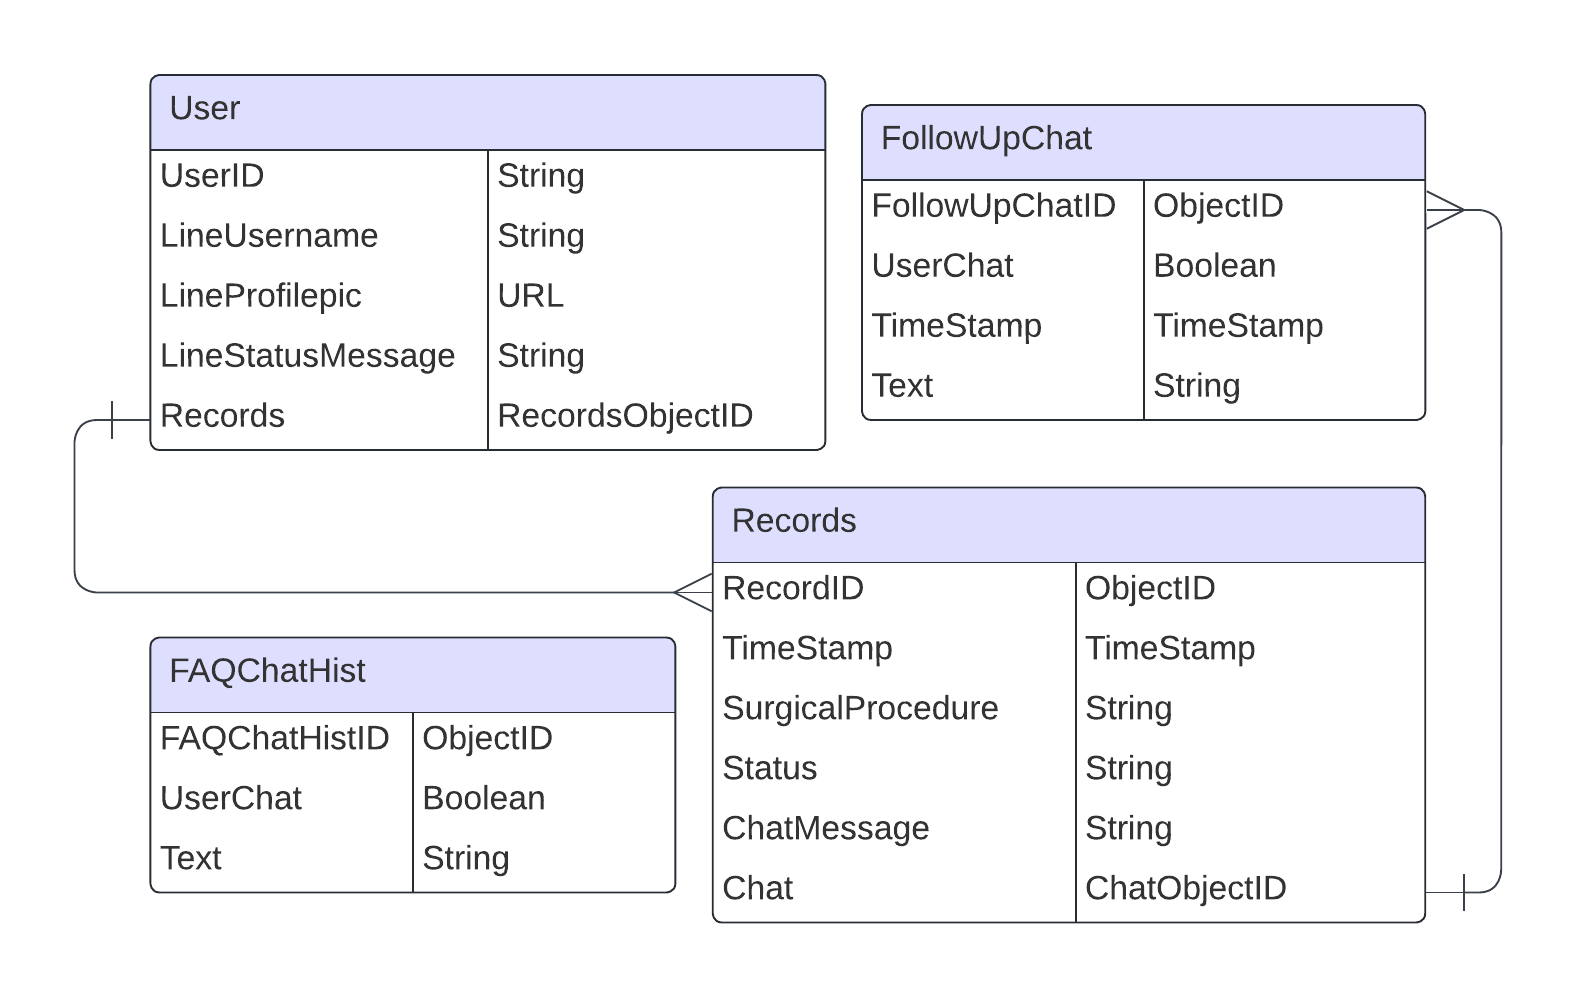
\includegraphics[width=.5\textwidth]{Image/ER.png}}
      \caption{ER-Diagram}\label{fig:ER}
      \begin{flushleft}
        \qquad Figure 3.10 shows the basic database design, which is required for store registered users. There are a total of 4 objects in our application. In the User object, it will have userID, Username, Profilepic, StatusMessage which is linked to Line profile. The User object will also contain  lists of RecordObject and FollowUpObject. In RecordsObject, there is RecordID, TimeStamp, SurgicalProcedure and Status. The RecordID is linked to the User object.  In FollowUp Object, there is FollowUpID, Title, TimeStamp, Chat and ChatResult. The FollowUpID is linked to the Record object and it is one to one relation. In ChatObject, there is ChatID, UserChat, TimeStamp, and Text. The ChatID is linked to the FollowUp object. \par
      \end{flushleft}
    \end{figure}
\newpage
  \section{User Interface}
    \subsection{Home Page}
    \begin{figure}[!h]
      \centering
      \begin{minipage}{.6\textwidth}
        \centering
        \fbox{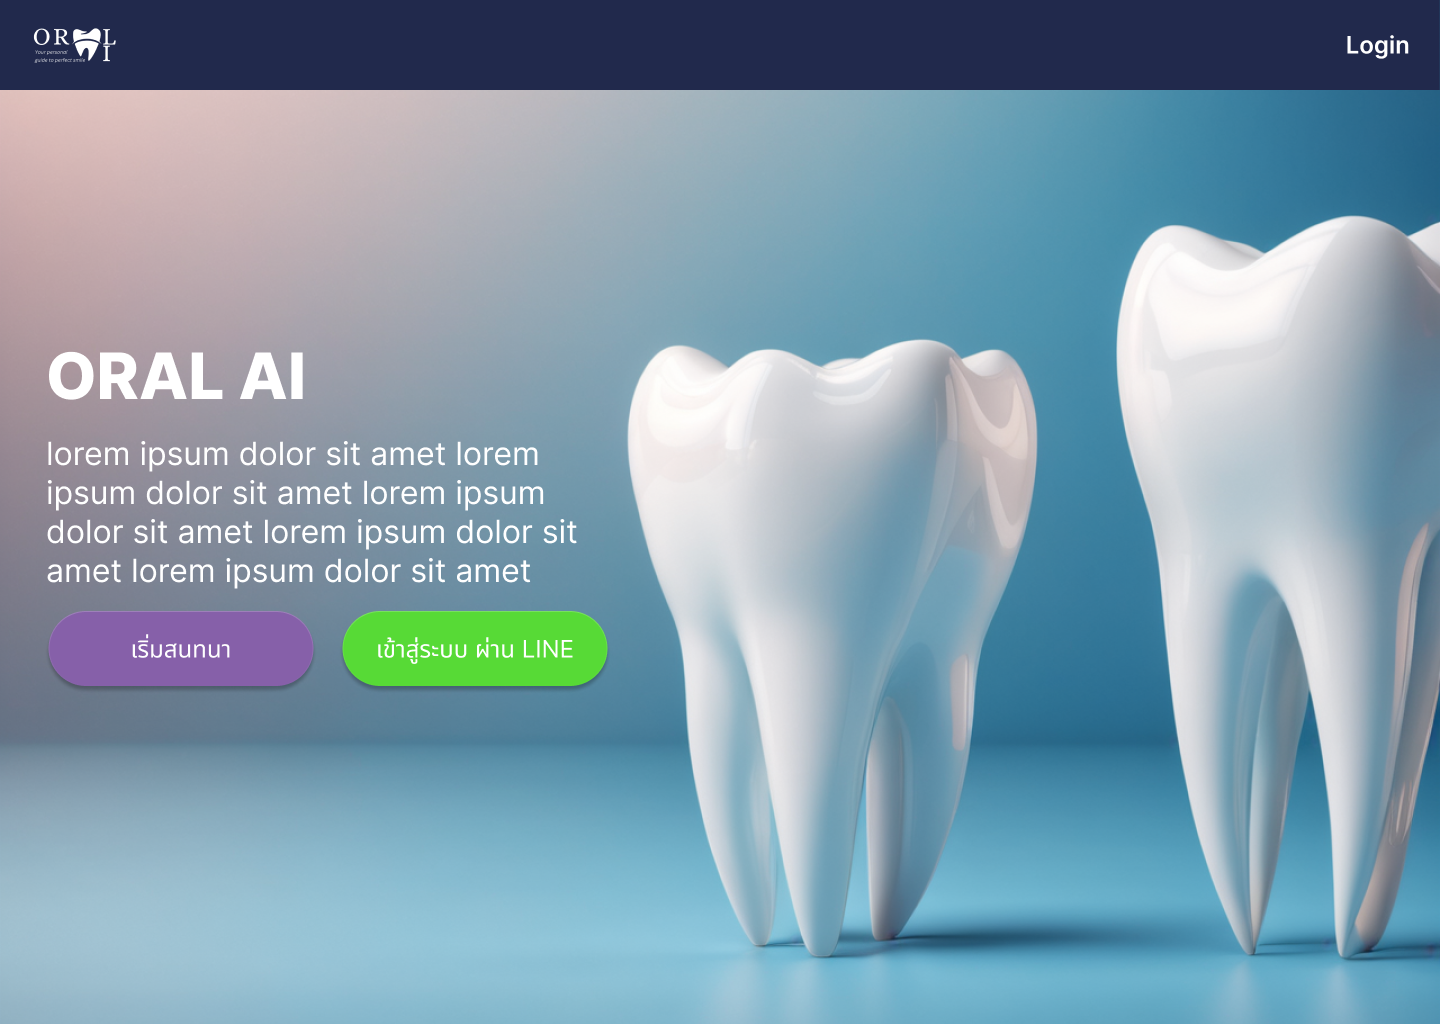
\includegraphics[width=.8\linewidth]{Image/Desk_Home.png}}
      \end{minipage}%
      \begin{minipage}{.3\textwidth}
        \centering
        \fbox{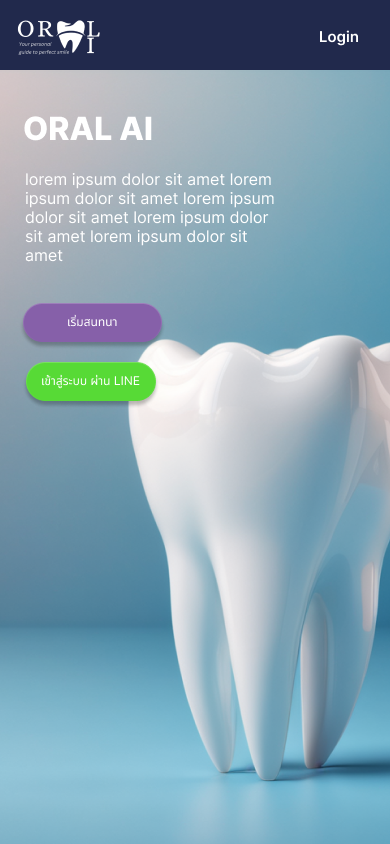
\includegraphics[width=.6\linewidth]{Image/Mob_Home.png}}
      \end{minipage}
      \caption{Website home page (Desktop and mobile respectively)}\label{fig:HomePage}
      \begin{flushleft}
        \qquad Figure 3.11 is the home page of the web application, this page will show a short description about our website and includes 2 buttons, Start Chatting and Login by Line. The Start Chatting button will take the user to the question answering page and Login by Line will link to the Line login page. \par
      \end{flushleft}
    \end{figure}

    \subsection{Follow-Up page}
      \begin{figure}[!h]
        \centering
        \fbox{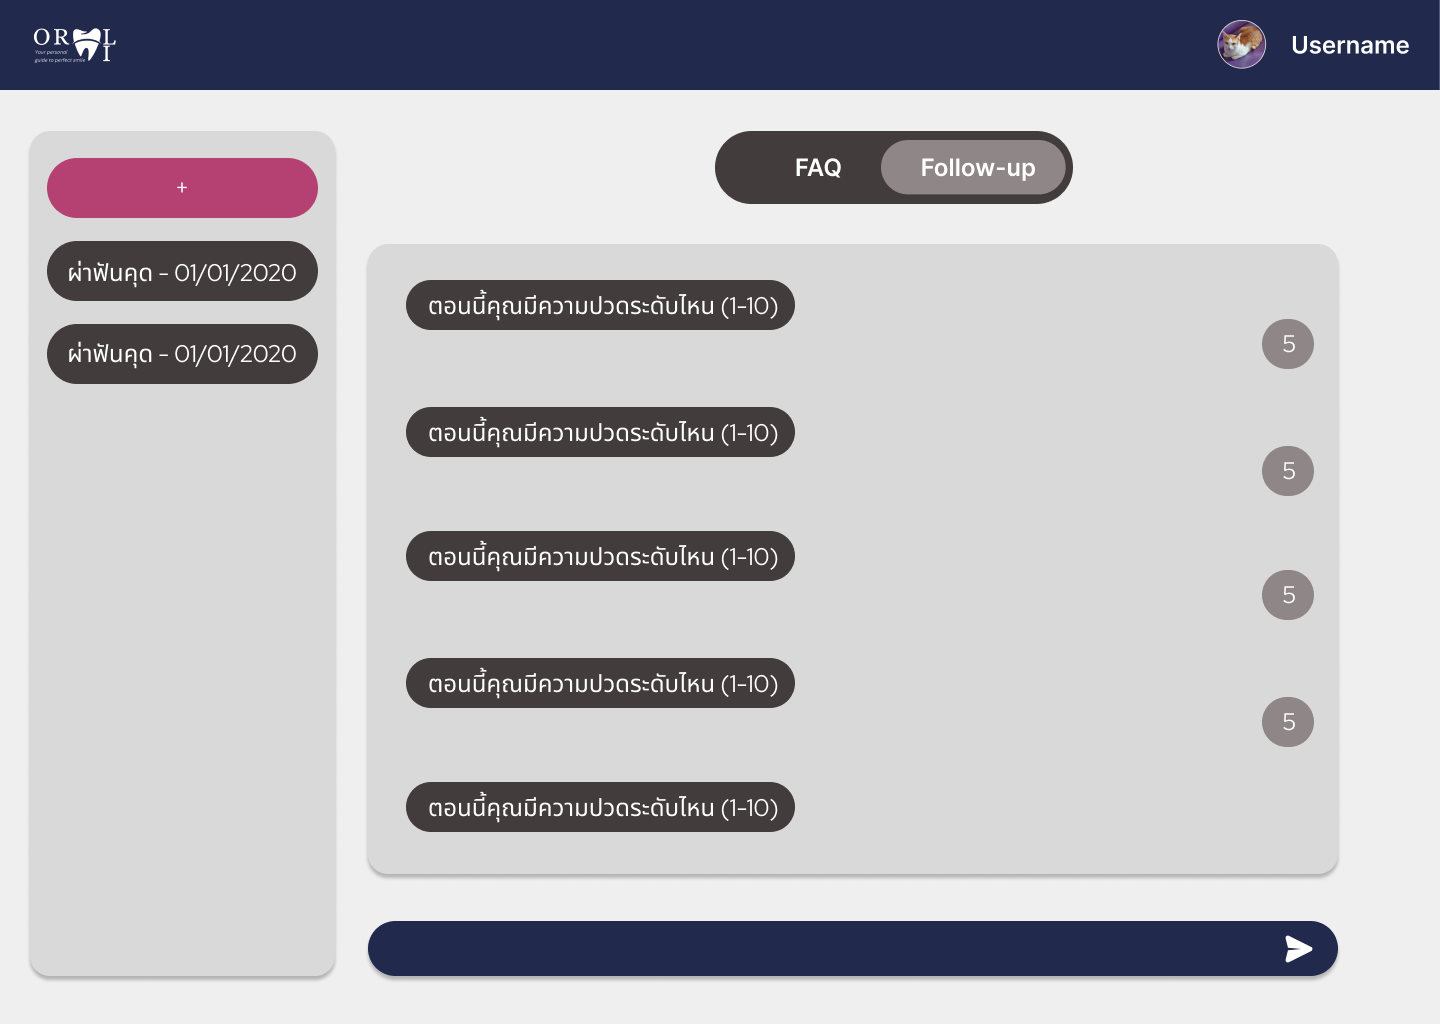
\includegraphics[width=.6\textwidth]{Image/Desk_Follow.png}}
        \caption{Desktop Follow-Up page}\label{fig:Desk_Follow}
        \begin{flushleft}
          \qquad Figure 3.12 is the Follow-Up page of the web application on desktop, this page includes case history in the left side of the page which is able to click to see follow-up chat history and chat box in the middle of the page, and input textbox under the chat box, and switch bar in the top of chat box use  for switch between FAQ and Follow-up feature. \par
        \end{flushleft}
      \end{figure}
\newpage
    \subsection{Follow-Up page}
    \begin{figure}[!h]
      \centering
      \begin{minipage}{.3\textwidth}
        \centering
        \fbox{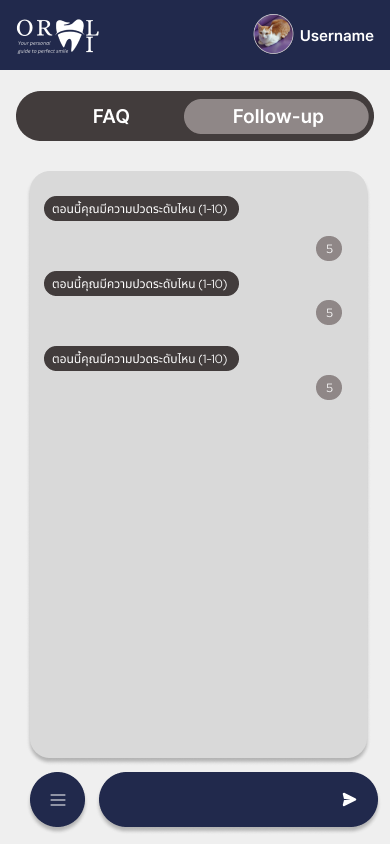
\includegraphics[width=.7\linewidth]{Image/Mob_Follow_1.png}}
      \end{minipage}%
      \begin{minipage}{.3\textwidth}
        \centering
        \fbox{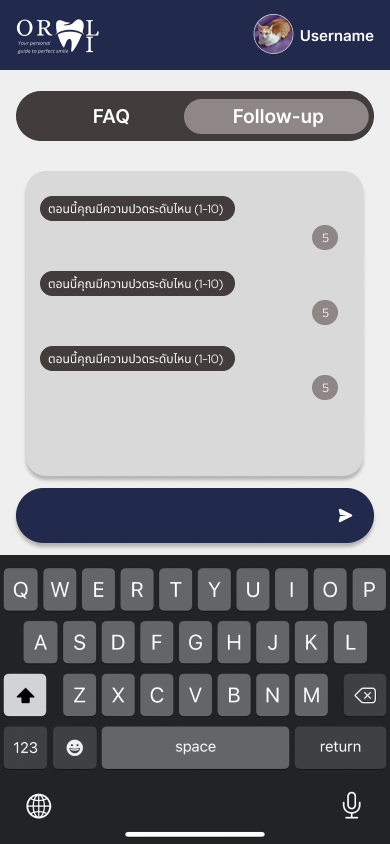
\includegraphics[width=.7\linewidth]{Image/Mob_Follow_2.png}}
      \end{minipage}%
      \begin{minipage}{.3\textwidth}
        \centering
        \fbox{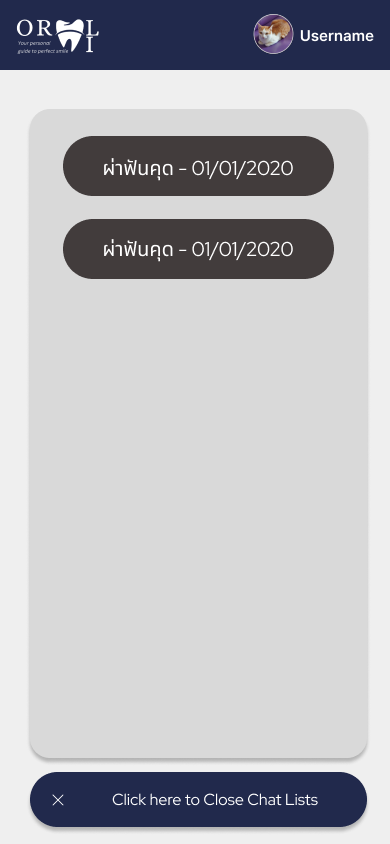
\includegraphics[width=.7\linewidth]{Image/Mob_Follow_3.png}}
      \end{minipage}
      \caption{Mobile Follow-Up page}\label{fig:Mob_Follow}
      \begin{flushleft}
        \qquad Figure 3.13 is the Follow-Up page of the web application on mobile, on the left is its normal state and on the center is when the keyboard is used. On the right is when the hamburger button is pressed, the keyboard input will be dismissed and be replaced with a long closed button to go back to its normal state. \par
      \end{flushleft}
    \end{figure}

    \subsection{FAQ page}
    \begin{figure}[!h]
      \centering
      \fbox{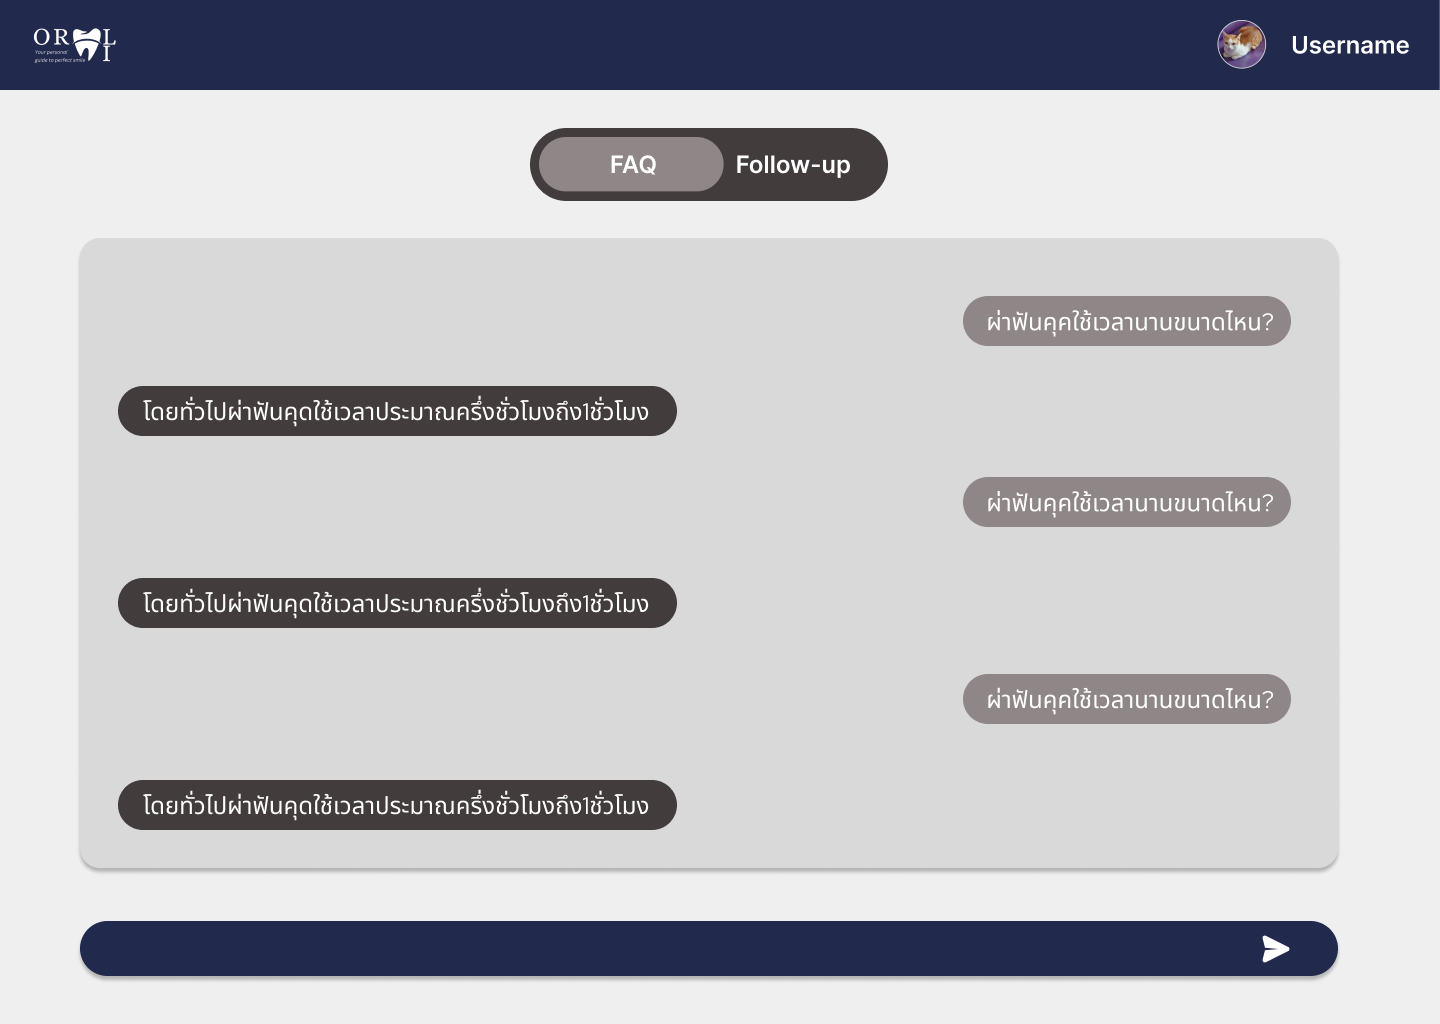
\includegraphics[width=.7\textwidth]{Image/Desk_FAQ.png}}
      \caption{Desktop Question Answering page}\label{fig:Desk_Follow}
      \begin{flushleft}
        \qquad Figure 3.14 is the Question Answering page of the web application on desktop, this page includes a chat box in the middle of the page and input textbox in the bottom and switch bar in the top of the chat box used for switching between FAQ and Follow-up feature. \par
      \end{flushleft}
    \end{figure}
\newpage
    \begin{figure}[!h]
      \centering
      \begin{minipage}{.3\textwidth}
        \centering
        \fbox{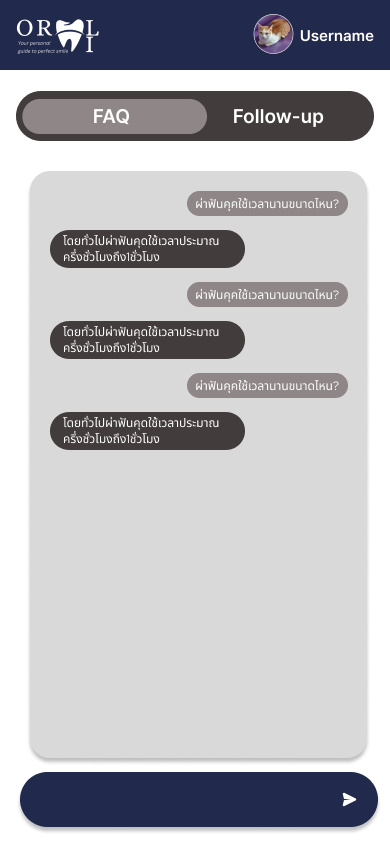
\includegraphics[width=.7\linewidth]{Image/Mob_FAQ_1.png}}
      \end{minipage}%
      \begin{minipage}{.3\textwidth}
        \centering
        \fbox{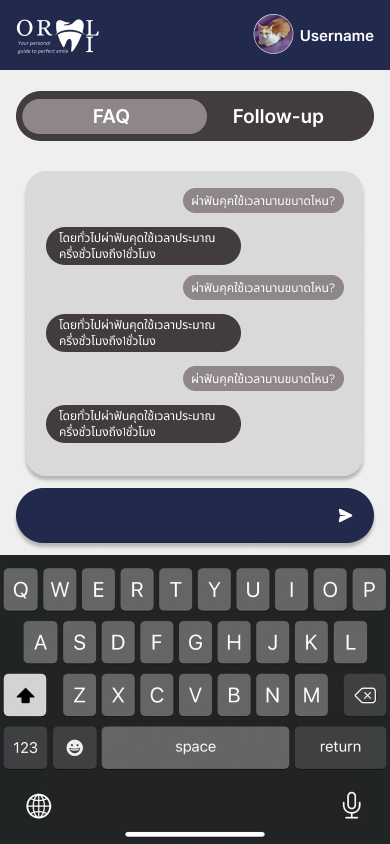
\includegraphics[width=.7\linewidth]{Image/Mob_FAQ_2.png}}
      \end{minipage}%
      \caption{Mobile Question Answering page}\label{fig:Mobile Question Answering page}
      \begin{flushleft}
        \qquad Figure 3.15 is the Question Answering page of the web application on desktop, on the left is its normal state and on the right is when the keyboard is used. \par
      \end{flushleft}
    \end{figure}

    \subsection{Patient Info page}
    \begin{figure}[!h]
      \centering
      \begin{minipage}{.7\textwidth}
        \centering
        \fbox{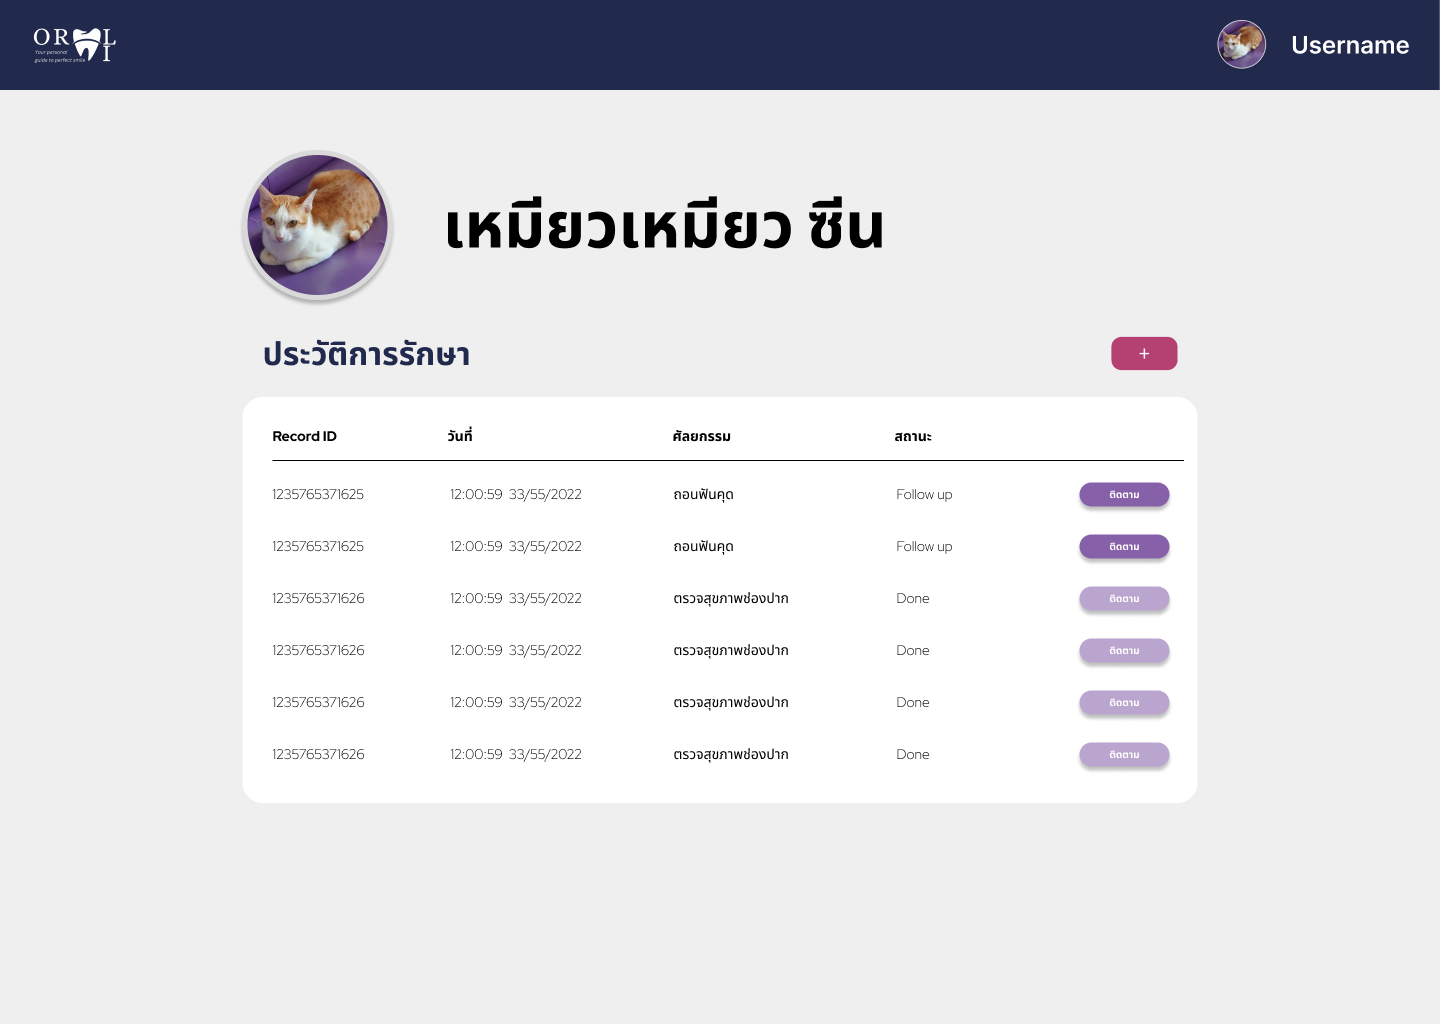
\includegraphics[width=.8\linewidth]{Image/Desk_Info.png}}
      \end{minipage}%
      \begin{minipage}{.25\textwidth}
        \centering
        \fbox{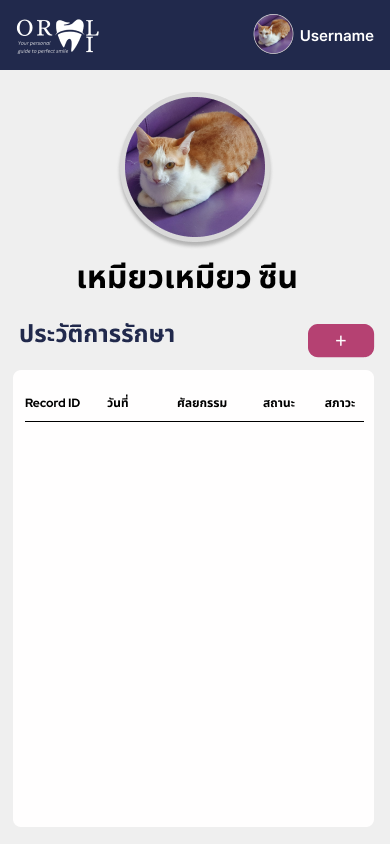
\includegraphics[width=.8\linewidth]{Image/Mob_Info.png}}
      \end{minipage}
      \caption{Patient Information page (Desktop and mobile respectively)}\label{fig:Patient Information page}
      \begin{flushleft}
        \qquad Figure 3.16 is the Patient Information page of the web application, it shows all the patient oral medical history that they registered. The record shows the record ID, Timestamp, Surgical Procedures type, status and the conditions. \par
      \end{flushleft}
    \end{figure}
\newpage
    \subsection{Line official page}
    \begin{figure}[!h]
      \centering
      \begin{minipage}{.3\textwidth}
        \centering
        \fbox{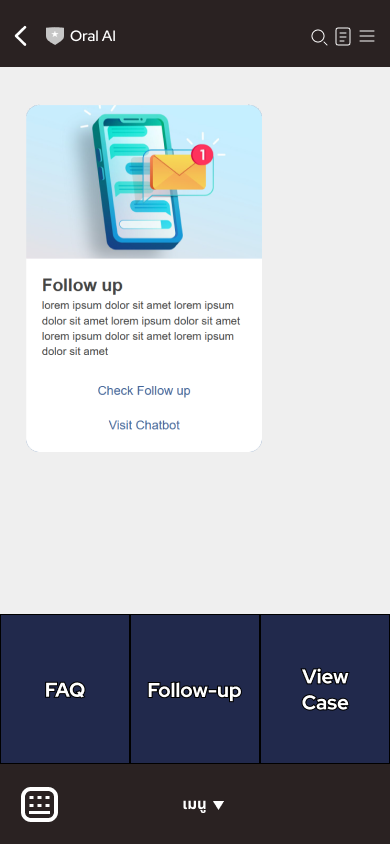
\includegraphics[width=.8\linewidth]{Image/Line_1.png}}
      \end{minipage}%
      \begin{minipage}{.3\textwidth}
        \centering
        \fbox{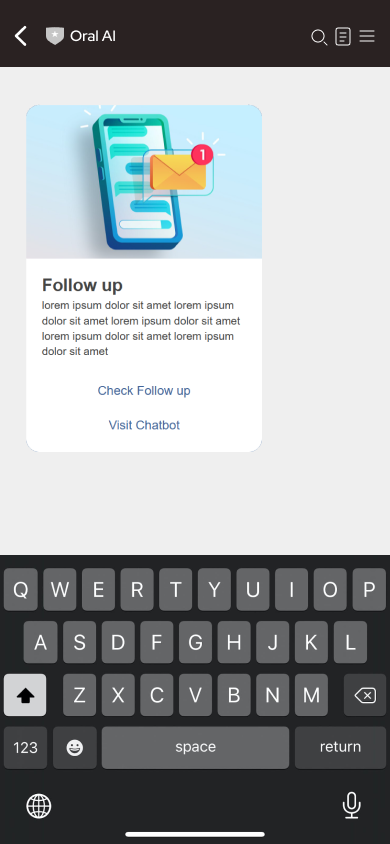
\includegraphics[width=.8\linewidth]{Image/Line_2.png}}
      \end{minipage}%
    
      \caption{Line Login Page}\label{fig:Line Login Page}
      \begin{flushleft}
        \qquad Figure 3.17 is how the line official page will look like, all notifications will be sent through here. The FAQ button will lead to the question answer website, Follow-up will lead to the follow up page of the website and view case will lead to the patient information page. \par
      \end{flushleft}
    \end{figure}
  \section{Evaluation Plan}
    \subsection{User Evaluation}
      \qquad After developing the platform in accordance with our goals , We will test our application and gather user feedback. We will collect the data about overall satisfaction, usability, user experience, and improvement suggestions. After the data has been collected, we will analyze and evaluate the application. \par
    \subsection{Application Evaluation}
      \qquad In assessing the performance of critical components, focus will be placed on two key metrics. First, Response Latency will be closely monitored the speed at which the chatbot responds to user queries. Additionally, Load Tests will be conducted to evaluate the system's capacity to handle user interactions. Furthermore, accuracy in providing precise and correct answers to dental queries ensures the chatbot's proficiency in delivering accurate information. \par

\chapter{EXPERIMENTAL RESULTS}
  \section{Dental Frequently Asked Question Collection}
    \qquad Since the project should be able to answer the input queries, we have gathered commonly asked questions about the 4 surgeries mentioned. We conducted surveys and consulted with experts to ensure accurate and appropriate answers. This section contains the questionnaire and its results. \par
    \subsection{Collection Process}
      \qquad The questions were gathered using Google Forms. The questionnaire below was created aimed to cover a wide range of opinions and concerns regarding dental health and medical treatments. Questions in the questionnaire consisted of \textthai{คุณเคยผ่านการรักษาหรือการผ่าตัดไหนมาแล้วบ้าง, สาเหตุที่คุณเข้ารับการรักษา/ผ่าตัด, คำถามที่มักจะเจอหรือสงสัยเกี่ยวกับโรคและการรักษา/ผ่าตัดข้างต้น, คำถามที่มักสงสัยหลังจากที่ได้รับการรักษา/ผ่าตัด.} \par
      \begin{figure}[!h]
        \centering
        \fbox{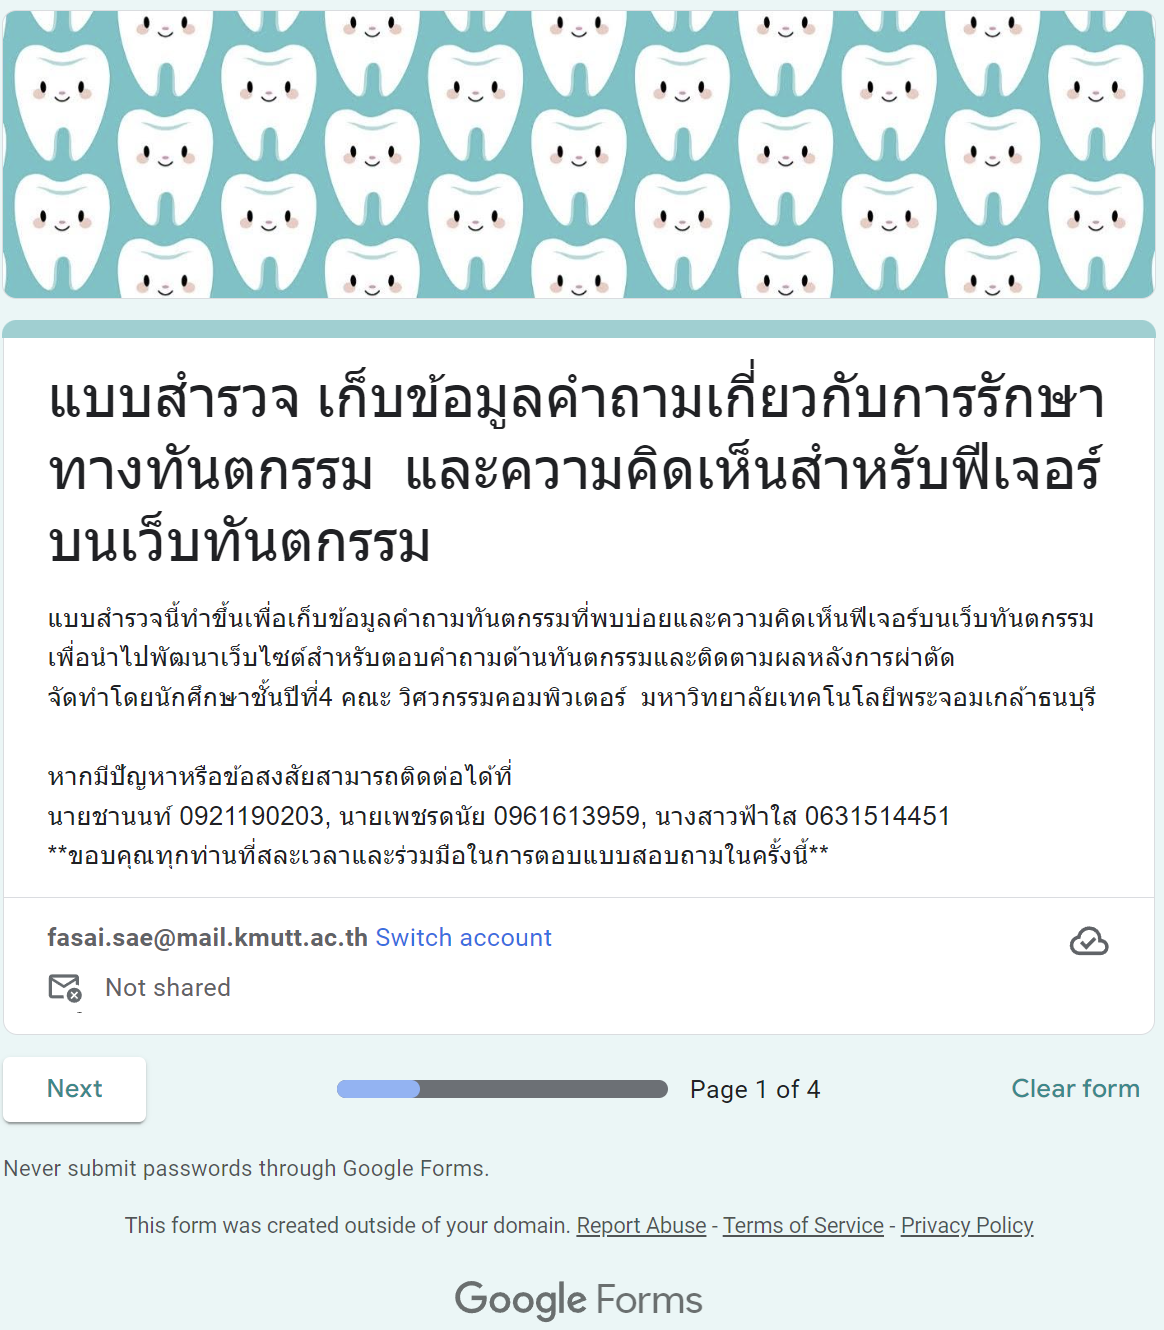
\includegraphics[width=.37\textwidth]{Image/Survey_1.png}}
        \caption{First page of the questionnaire}\label{fig:Survey_1}
      \end{figure}
      \begin{figure}[!h]
        \centering
        \fbox{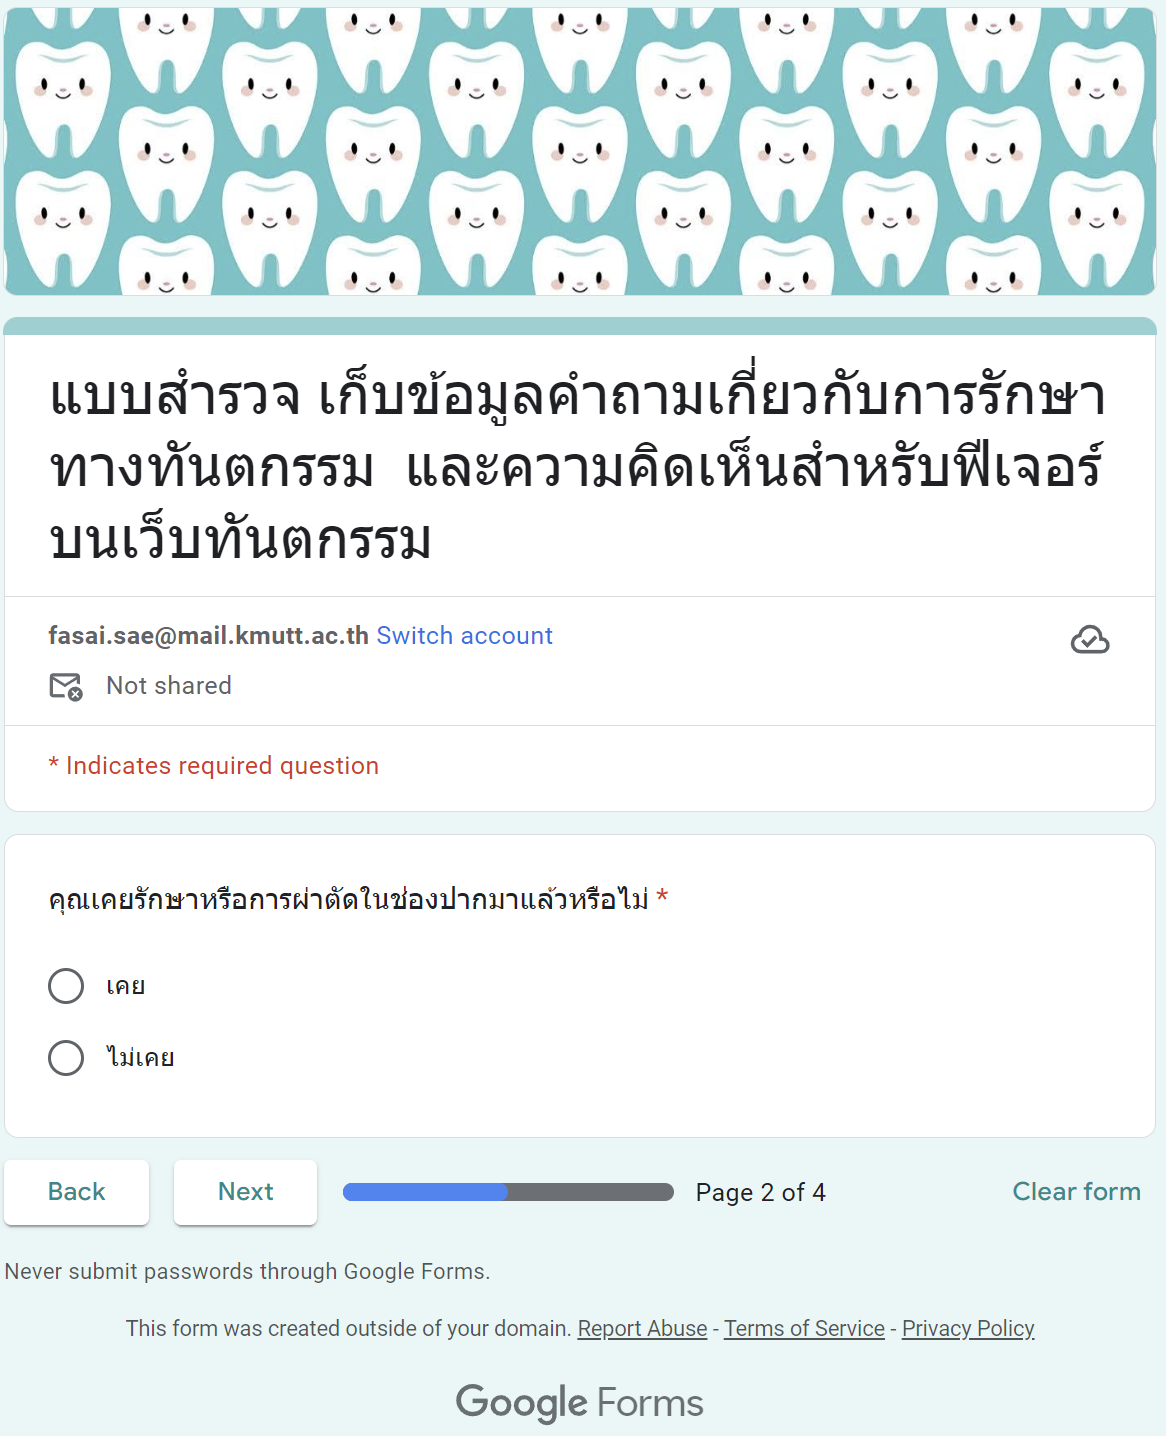
\includegraphics[width=.37\textwidth]{Image/Survey_2.png}}
        \caption{Second page of the questionnaire}\label{fig:Survey_2}
      \end{figure}
      \begin{figure}[!h]
        \centering
        \fbox{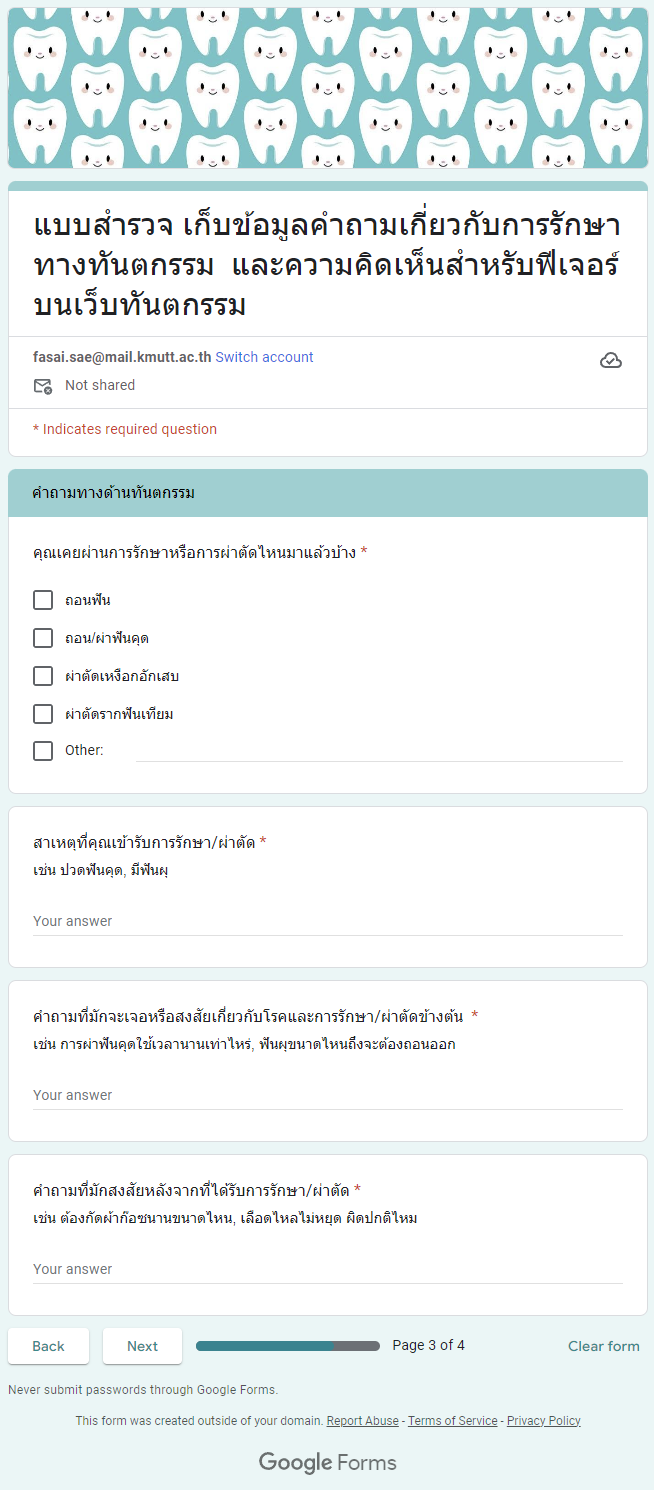
\includegraphics[width=.4\textwidth]{Image/Survey_3.png}}
        \caption{Third page of the questionnaire}\label{fig:Survey_3}
      \end{figure}
      \begin{figure}[!h]
        \centering
        \fbox{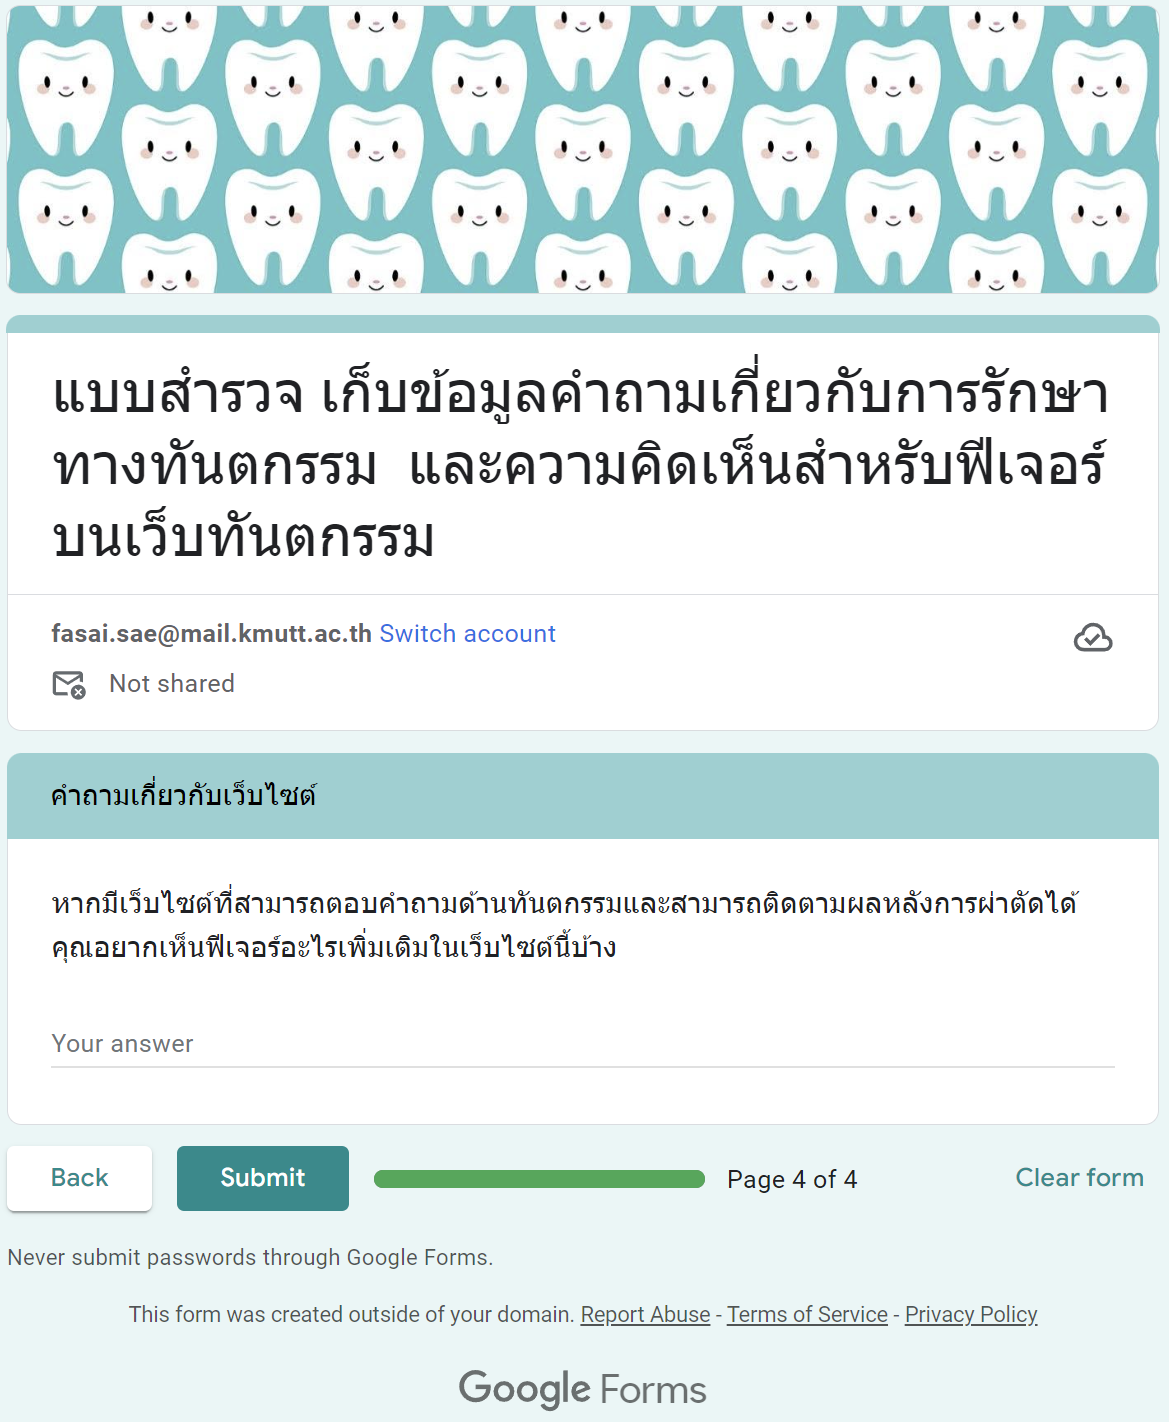
\includegraphics[width=.4\textwidth]{Image/Survey_4.png}}
        \caption{Fourth page of the questionnaire}\label{fig:Survey_4}
      \end{figure}
      \FloatBarrier{}
    \subsection{Results}
      \begin{figure}[!h]
        \centering
        \fbox{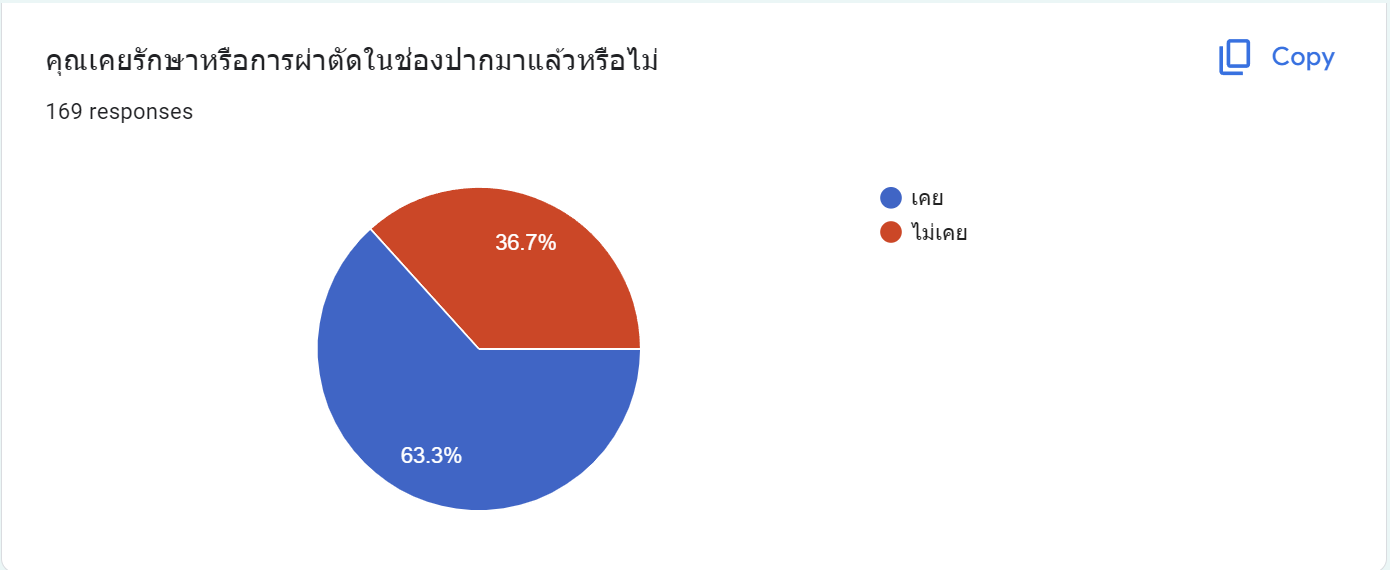
\includegraphics[width=.5\textwidth]{Image/Result_1.png}}
        \caption{Pie chart of Distribution of Oral Surgery Experience}\label{fig:Result_1}
      \end{figure}
      \begin{figure}[!h]
        \centering
        \fbox{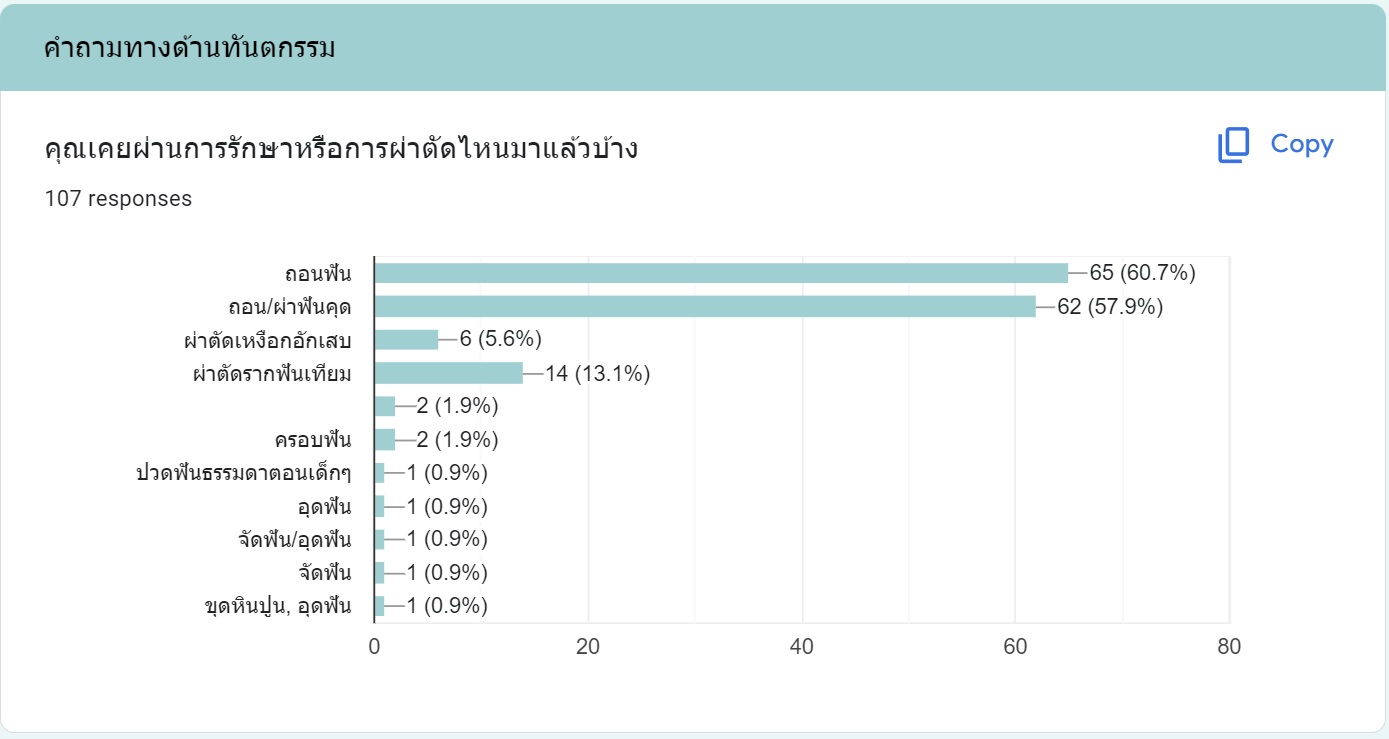
\includegraphics[width=.5\textwidth]{Image/Result_2.png}}
        \caption{Respondent’s Oral Surgeries Experience}\label{fig:Result_2}
      \end{figure}
      \begin{figure}[!h]
        \centering
        \fbox{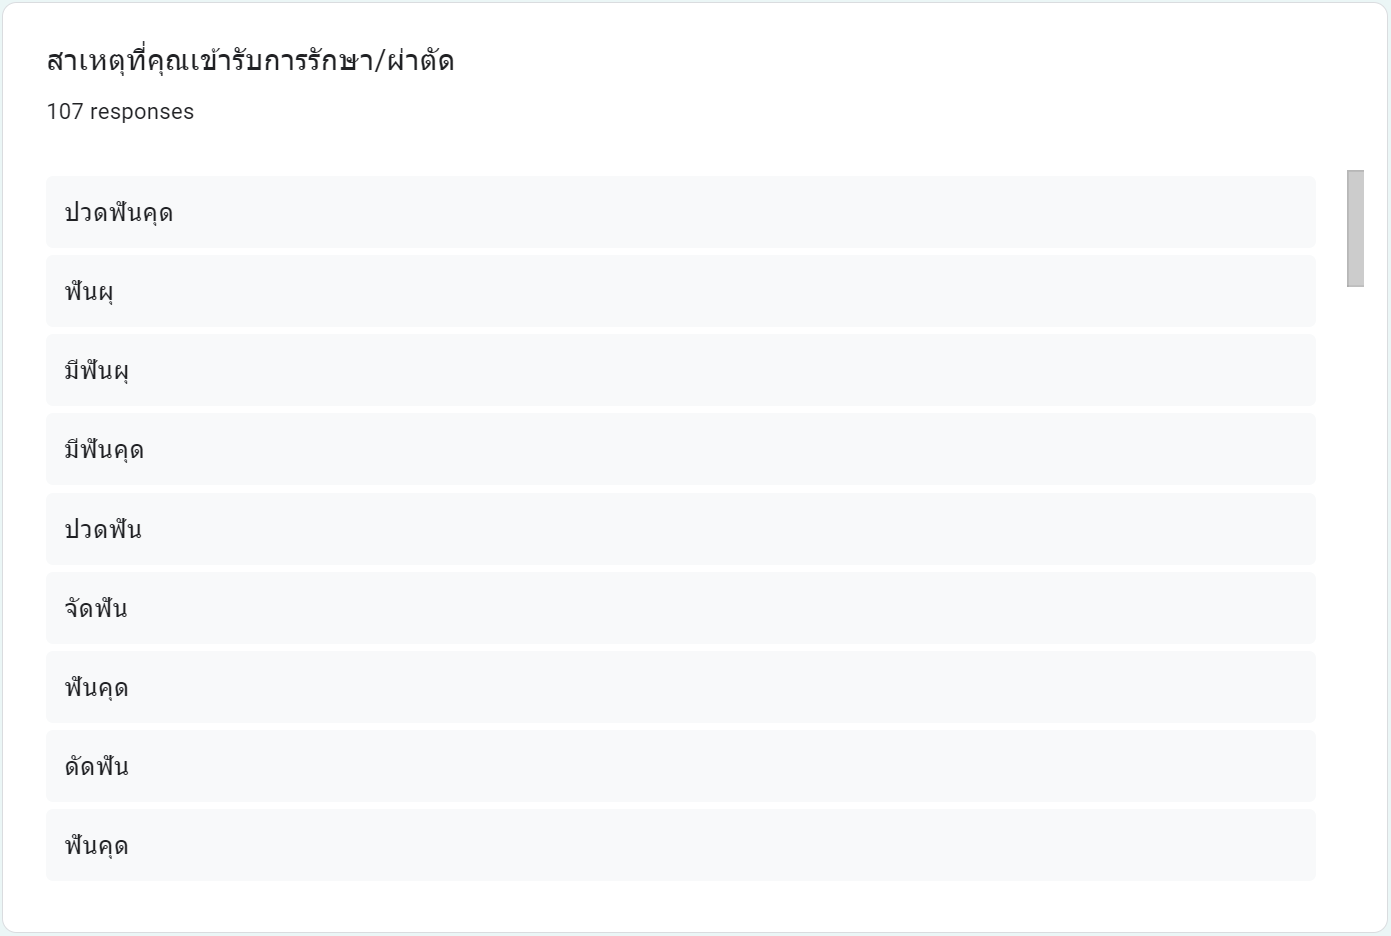
\includegraphics[width=.5\textwidth]{Image/Result_3.png}}
        \caption{Reason the Respondent Attend the Treatment}\label{fig:Result_3}
      \end{figure}
      \begin{figure}[!h]
        \centering
        \fbox{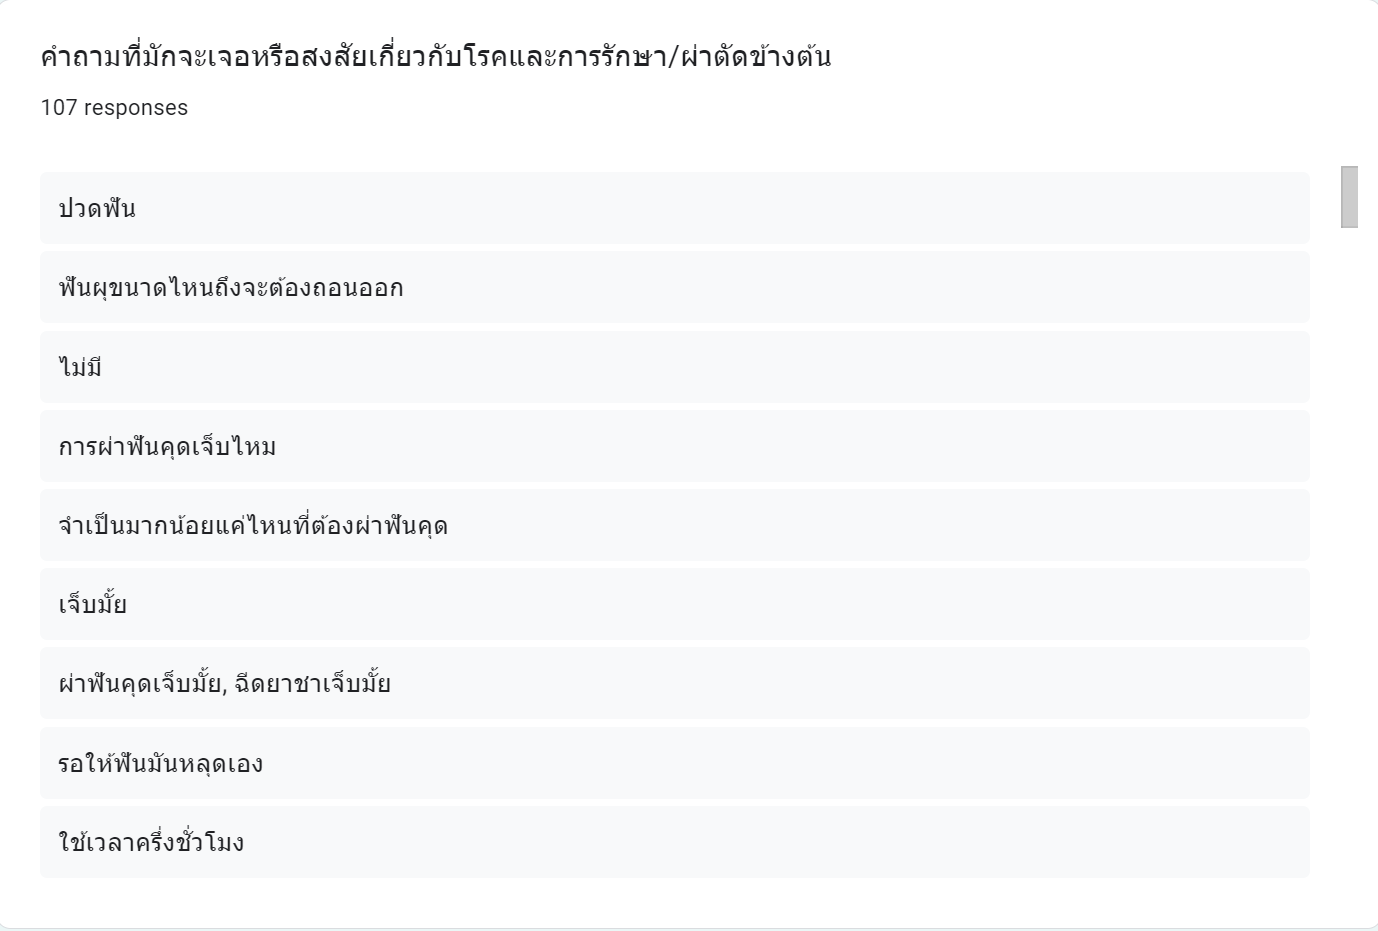
\includegraphics[width=.5\textwidth]{Image/Result_4.png}}
        \caption{Common Questions and Concerns About Surgeries and Treatment}\label{fig:Result_4}
      \end{figure}
      \begin{figure}[!h]
        \centering
        \fbox{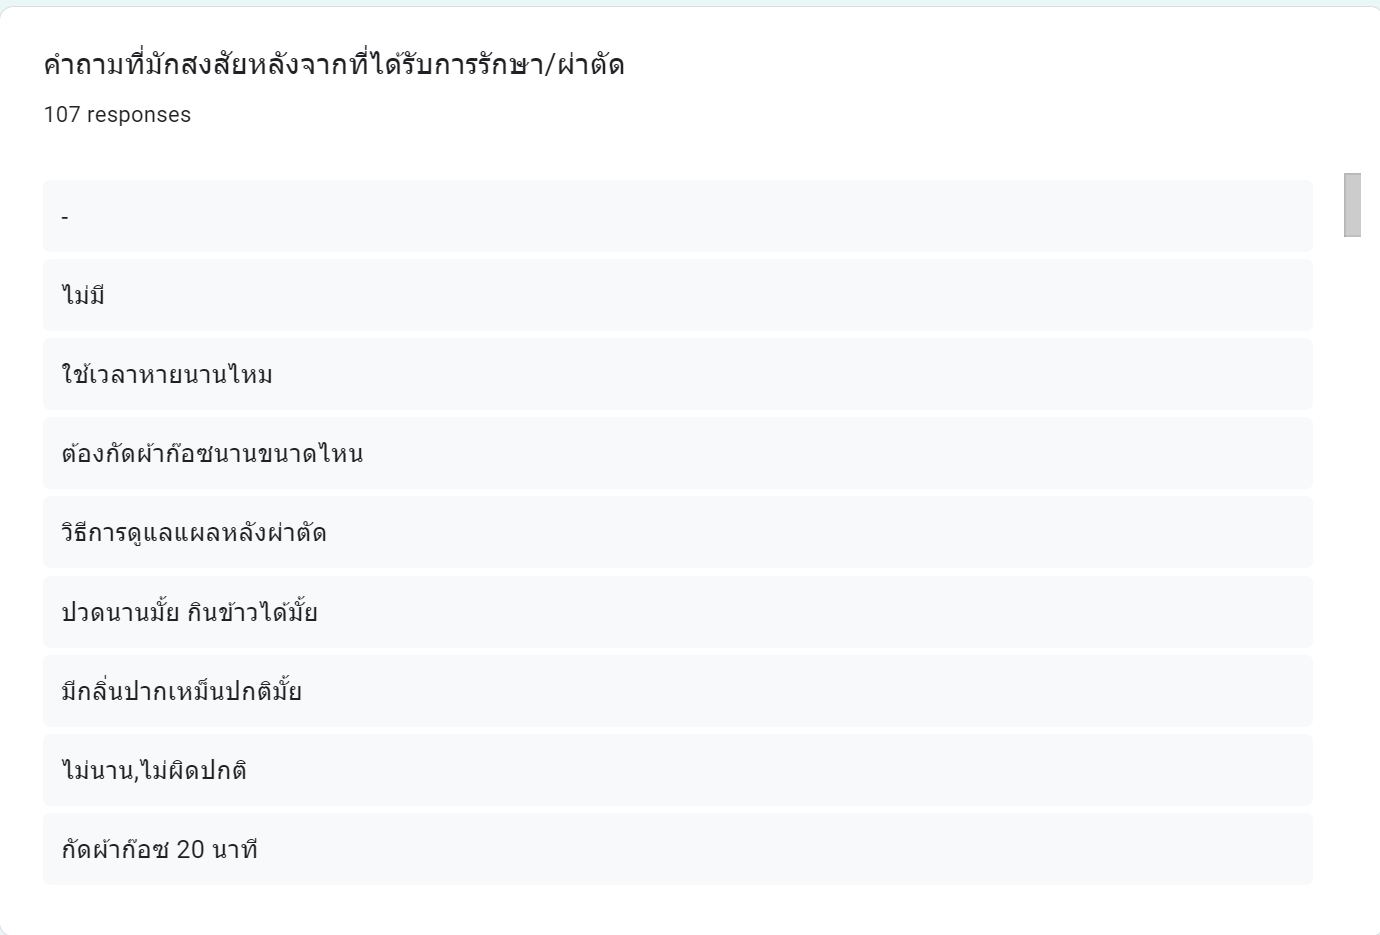
\includegraphics[width=.5\textwidth]{Image/Result_5.png}}
        \caption{Post-Treatment Frequently Asked Questions}\label{fig:Result_5}
      \end{figure}
      \begin{figure}[!h]
        \centering
        \fbox{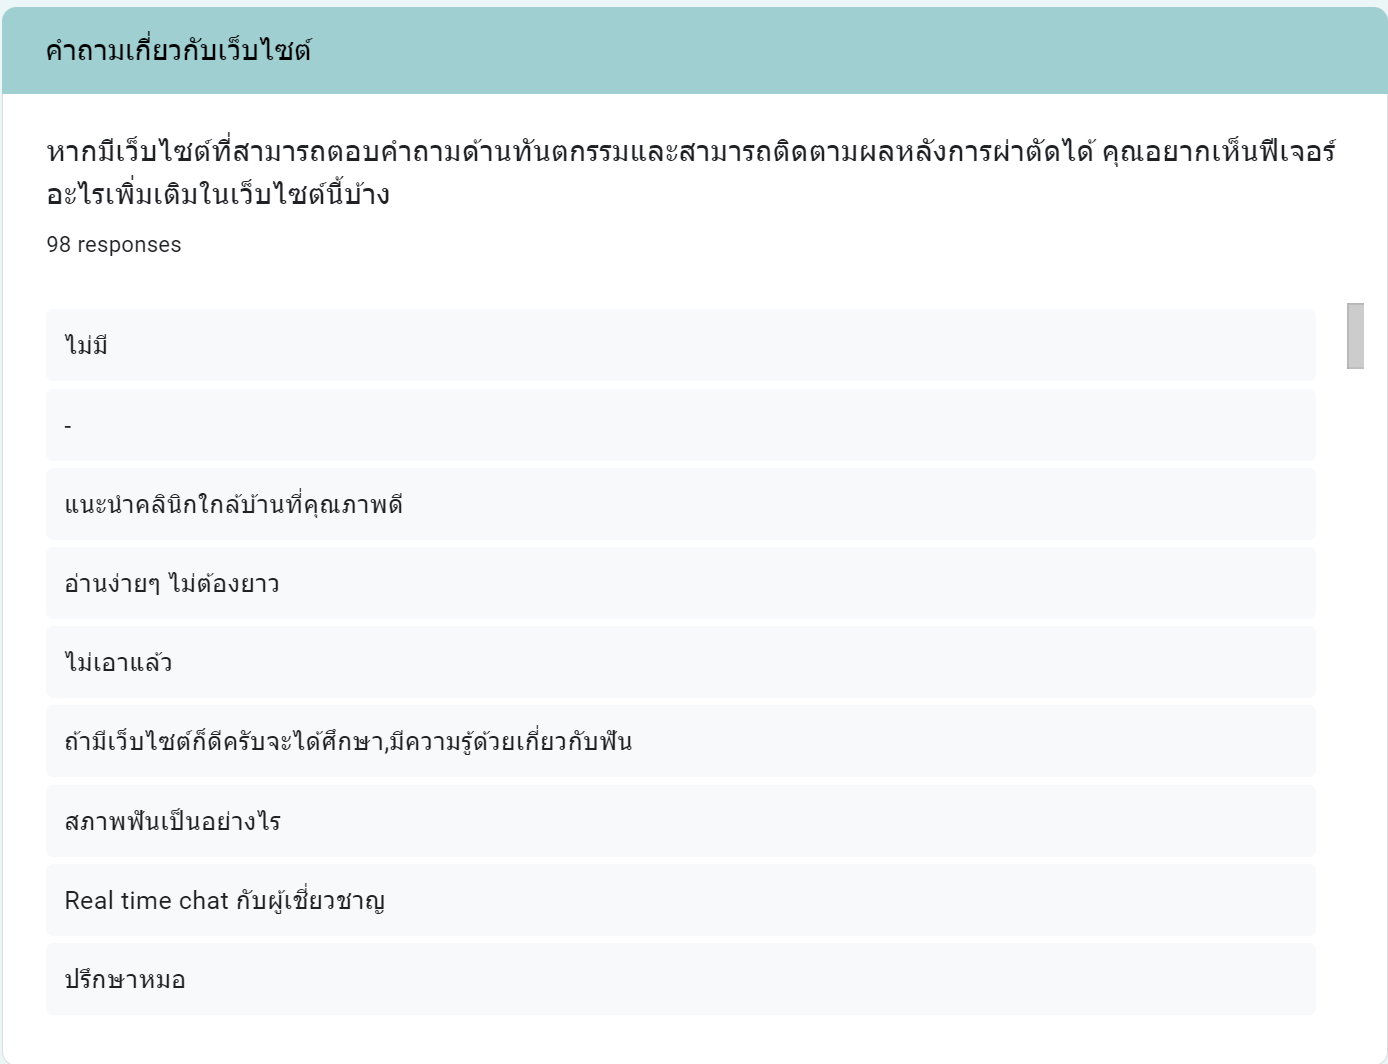
\includegraphics[width=.5\textwidth]{Image/Result_6.png}}
        \caption{Recommendations for Website Development and Features}\label{fig:Result_6}
      \end{figure}
      \FloatBarrier{}

  \section{Follow-Up Procedure Interview}
    \qquad Since the follow-up process is one of the project's main features, we must examine every important aspect in order to emphasize the post-surgery follow-up in the context of dental healthcare, understand the importance of comprehensive patient care, as well as the details of the follow-up process. This will allow us to imitate the actual medical staff procedure. This section explains how we conducted interviews with the dental clinic's medical staff in order to gain important insights into the techniques used for post-surgery tracking. \par
    \subsection{Interviewing Dental Clinic Around the University}
      \qquad To gain an insight and understand post-surgery follow-up procedure, we have first conducted an interview at the dental clinic around the university. The interview question include question such as \textthai{ขั้นตอนการติดตามอาการผู้ป่วย, โดยปกติแล้วจะทำการโทรติดตามอาการคนไข้กี่ชั่วโมงหลังผ่าตัด, คำถามที่มักจะถามผู้ป่วยตอนติดตามอาการ, คำถามที่ผู้ป่วยมักจะถามกลับมา.} After these interviews, we have gained invaluable insights and a deeper understanding of the follow-up procedures, enhancing our research with firsthand perspectives on patient care in the post-surgical phase within the local dental healthcare landscape. \par
    \subsection{Interviewing and Survey at Faculty of Dentistry at Chulalongkorn University}
      \qquad According to the important requirement for an in-depth understanding of the practicalities involved with the follow-up procedure, we needed to familiarize ourselves with the patient's involvement following surgery. This includes an in-depth investigation of  complexity of questions, symptom assessment, patient interaction during the follow-up phase, and response to particular concerns. Regarding the complexity of these interactions, we think it is important to have discussions and obtain advice from professionals, especially those who have experience with the follow-up procedure, and patient communication. \par
      \qquad In order to capture the view of the expert and  match our project with the actual demands of both medical professionals and patients, we conduct an on-site observation and interviews at the Faculty of Dentistry, Chulalongkorn University. \par
      \begin{figure}[!h]
        \centering
        \fbox{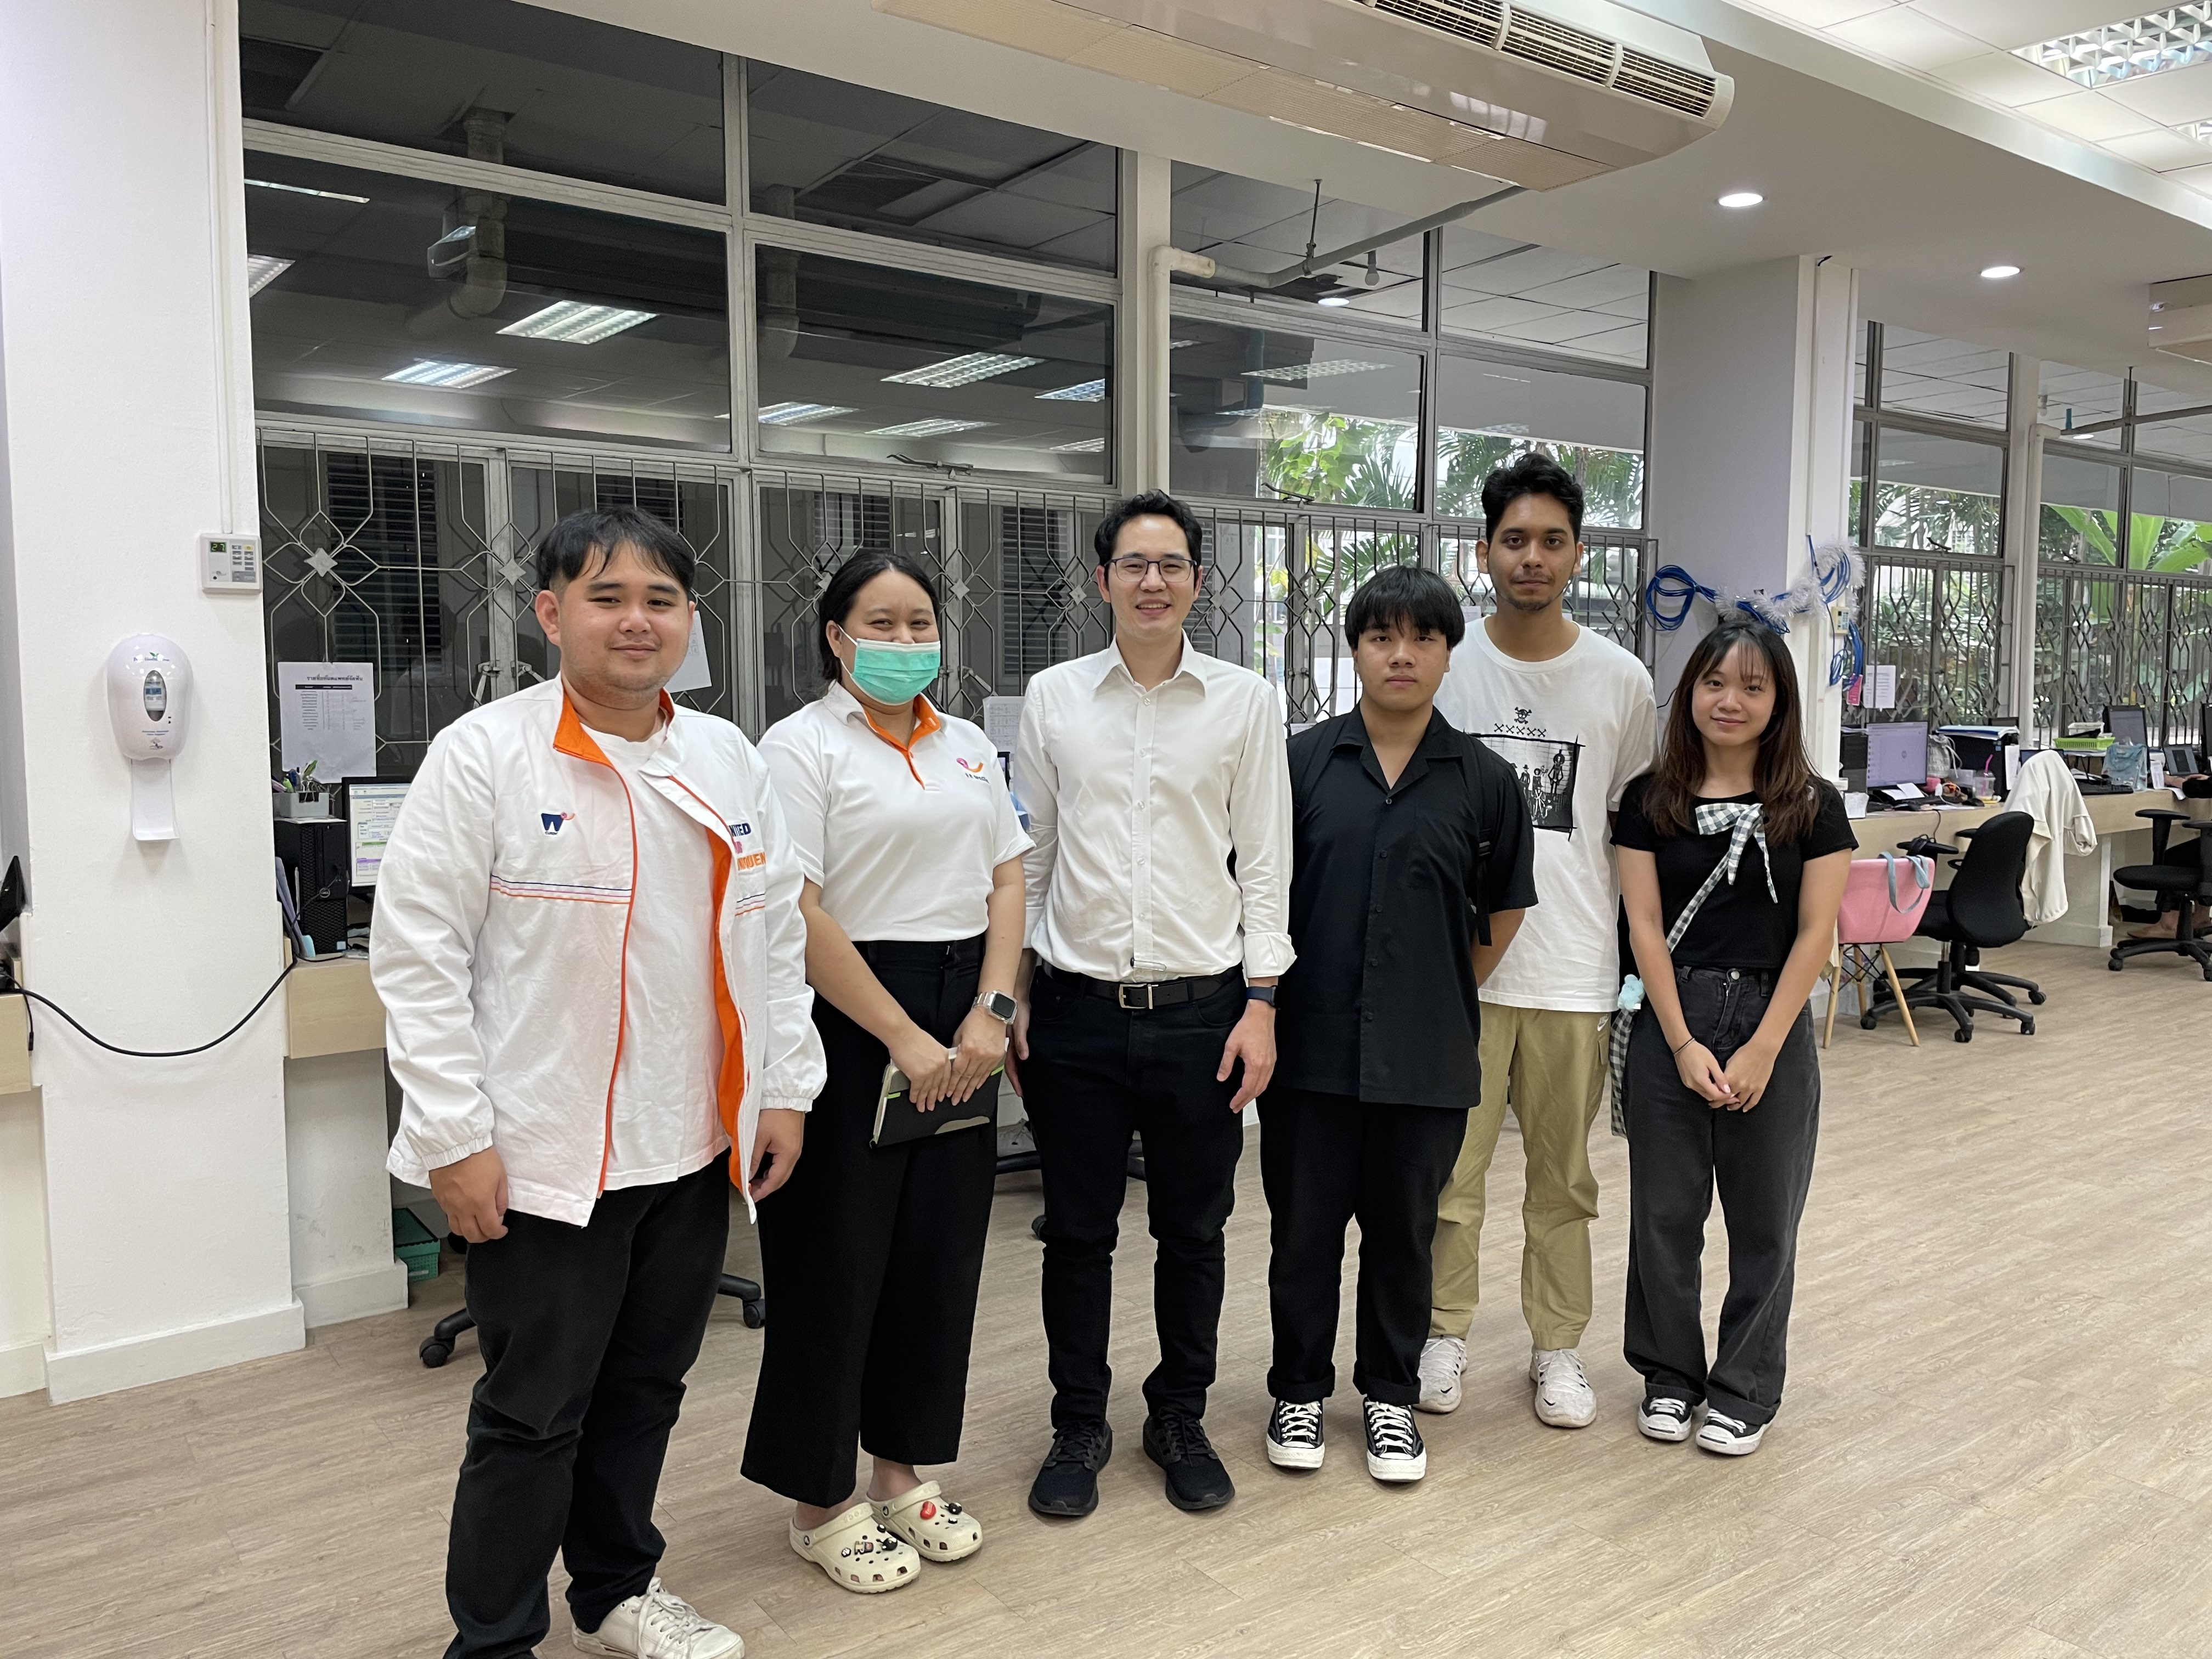
\includegraphics[width=.8\textwidth]{Image/Interview_1.jpg}}
        \caption{Our team and the call-center representative}\label{fig:Interview_1}
        \begin{flushleft}
          \qquad The call-center representative works at the OPD Instant Clinic's call center. The department is in charge of answering questions and helping out OPD patients. \par
        \end{flushleft}        
      \end{figure}
      \begin{figure}[!h]
        \centering
        \fbox{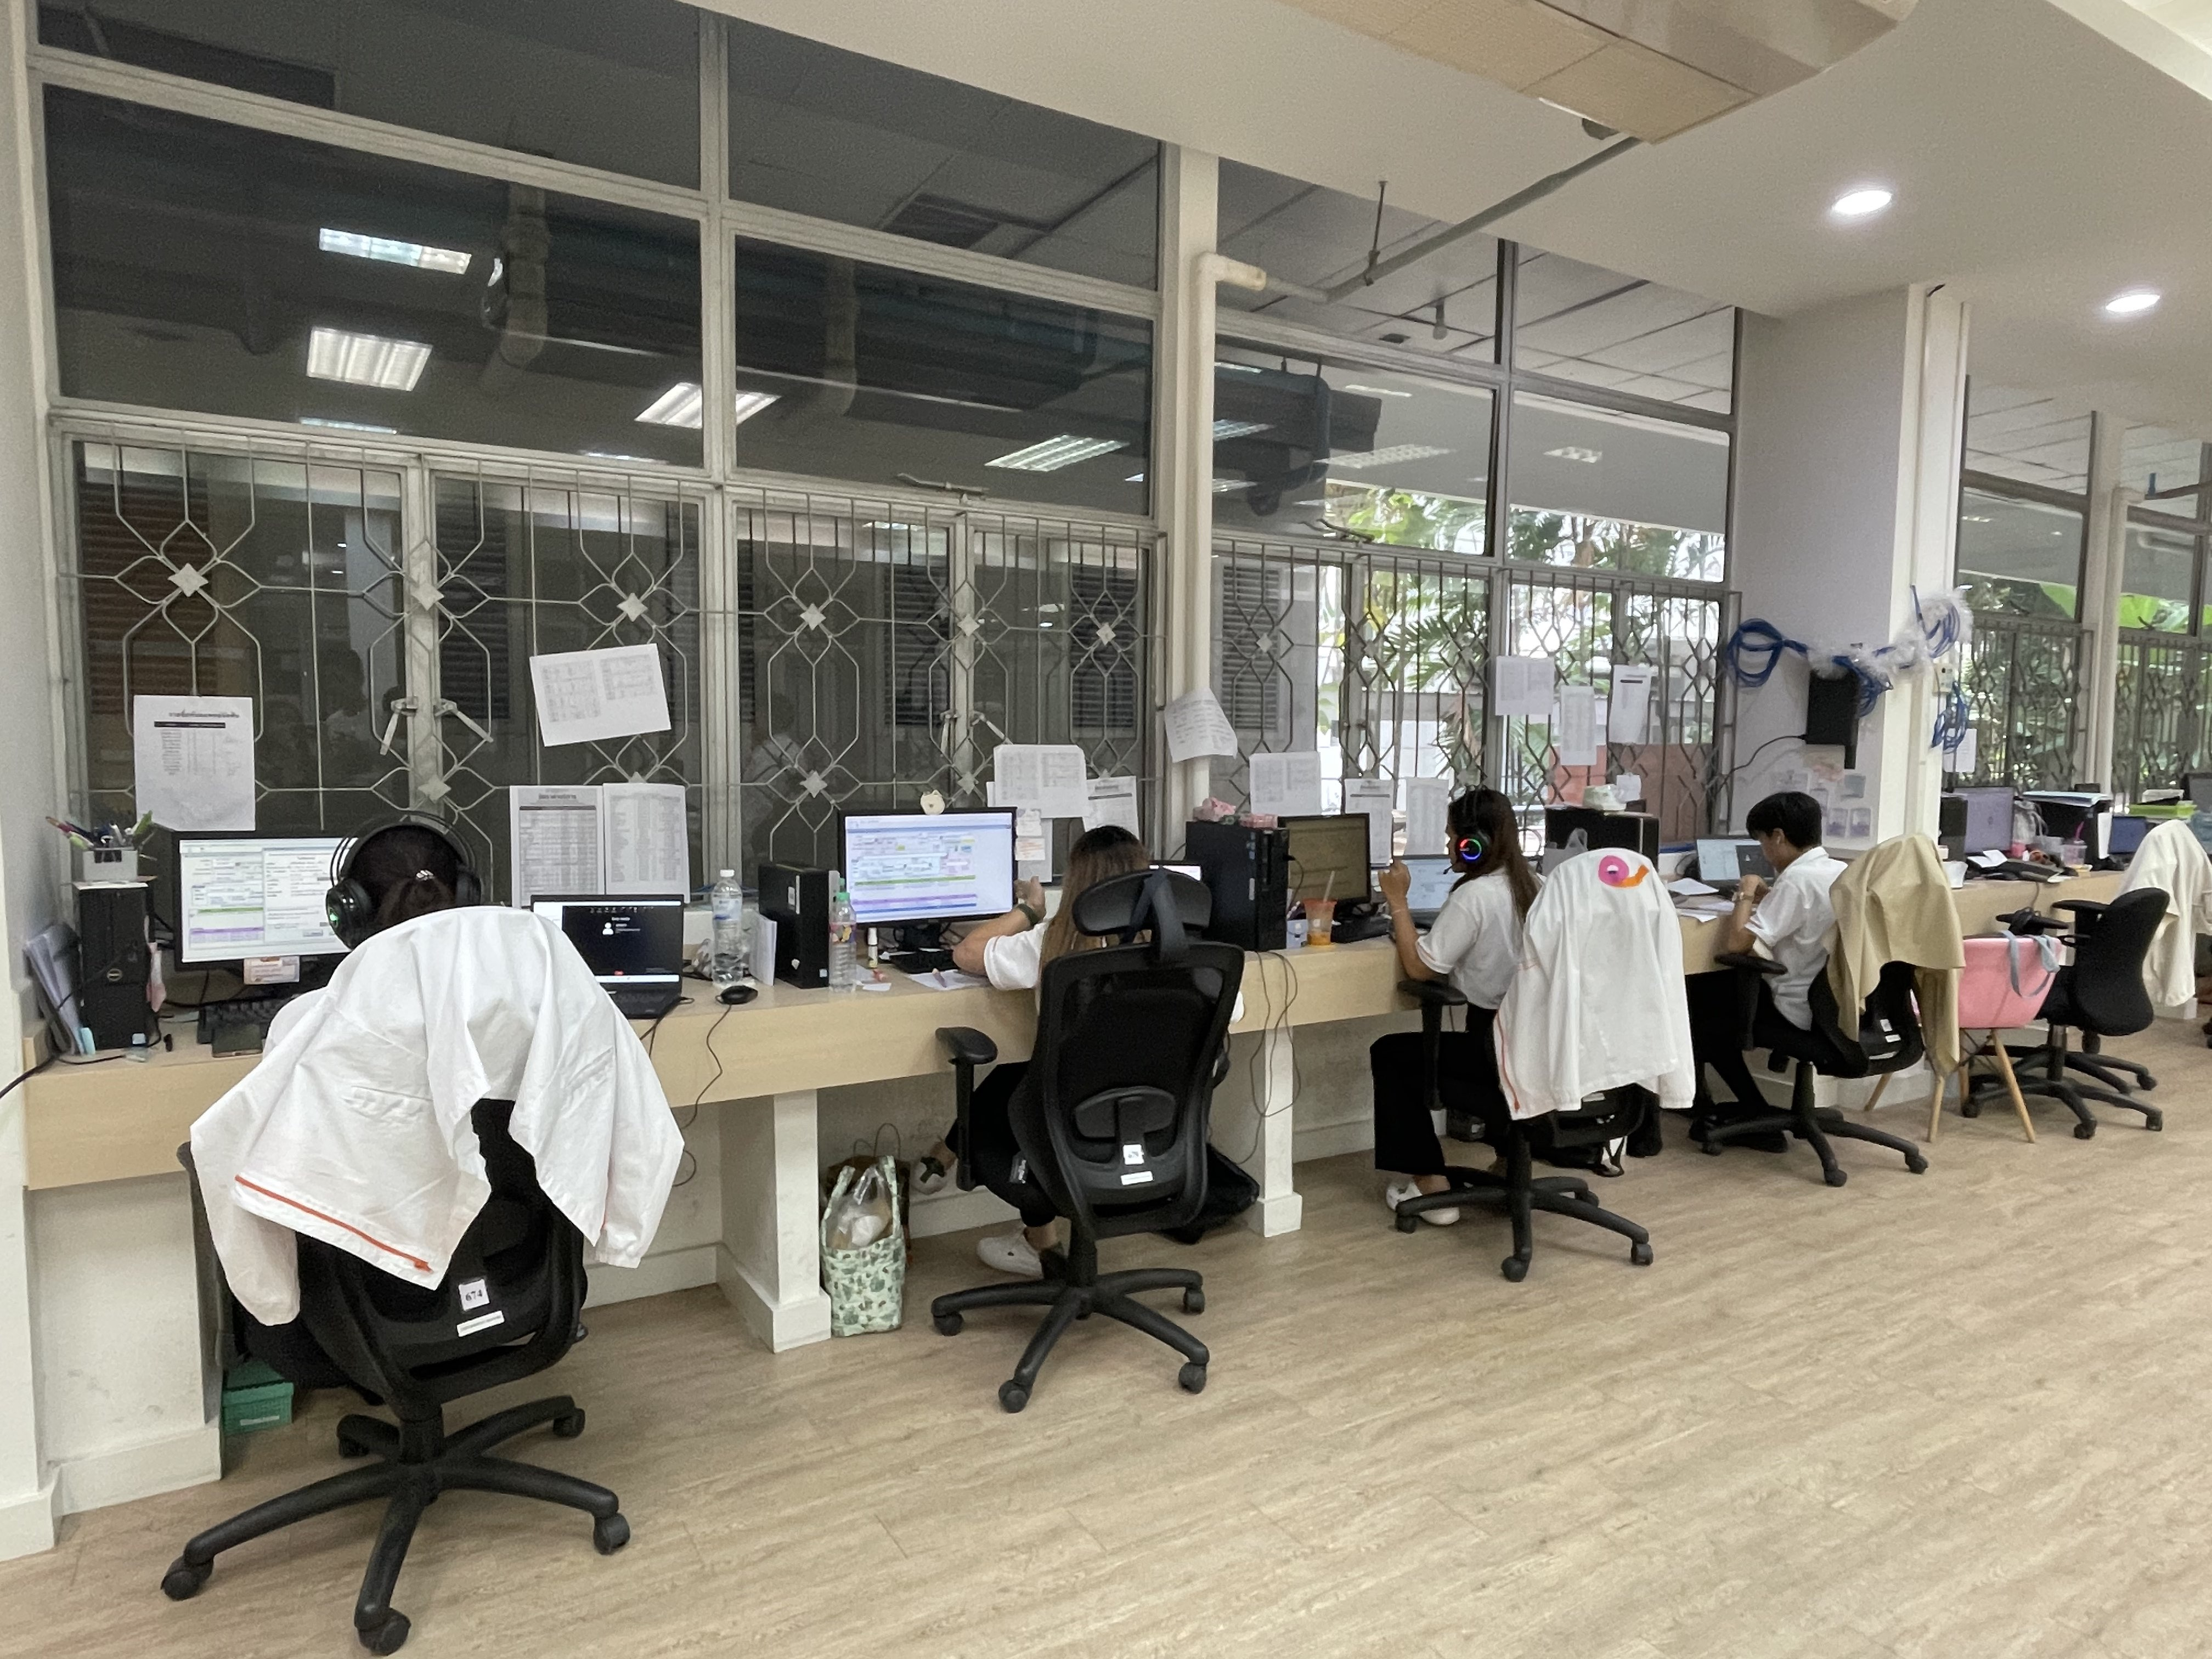
\includegraphics[width=.8\textwidth]{Image/Interview_2.jpg}}
        \caption{Working environment of the OPD Instant Clinic's call center}\label{fig:Interview_2}
        \begin{flushleft}
          \qquad The OPD Instant Clinic's call center is following-up with their patient a day after the surgeries. \par
        \end{flushleft}
      \end{figure}
      \begin{figure}
        \centering
        \fbox{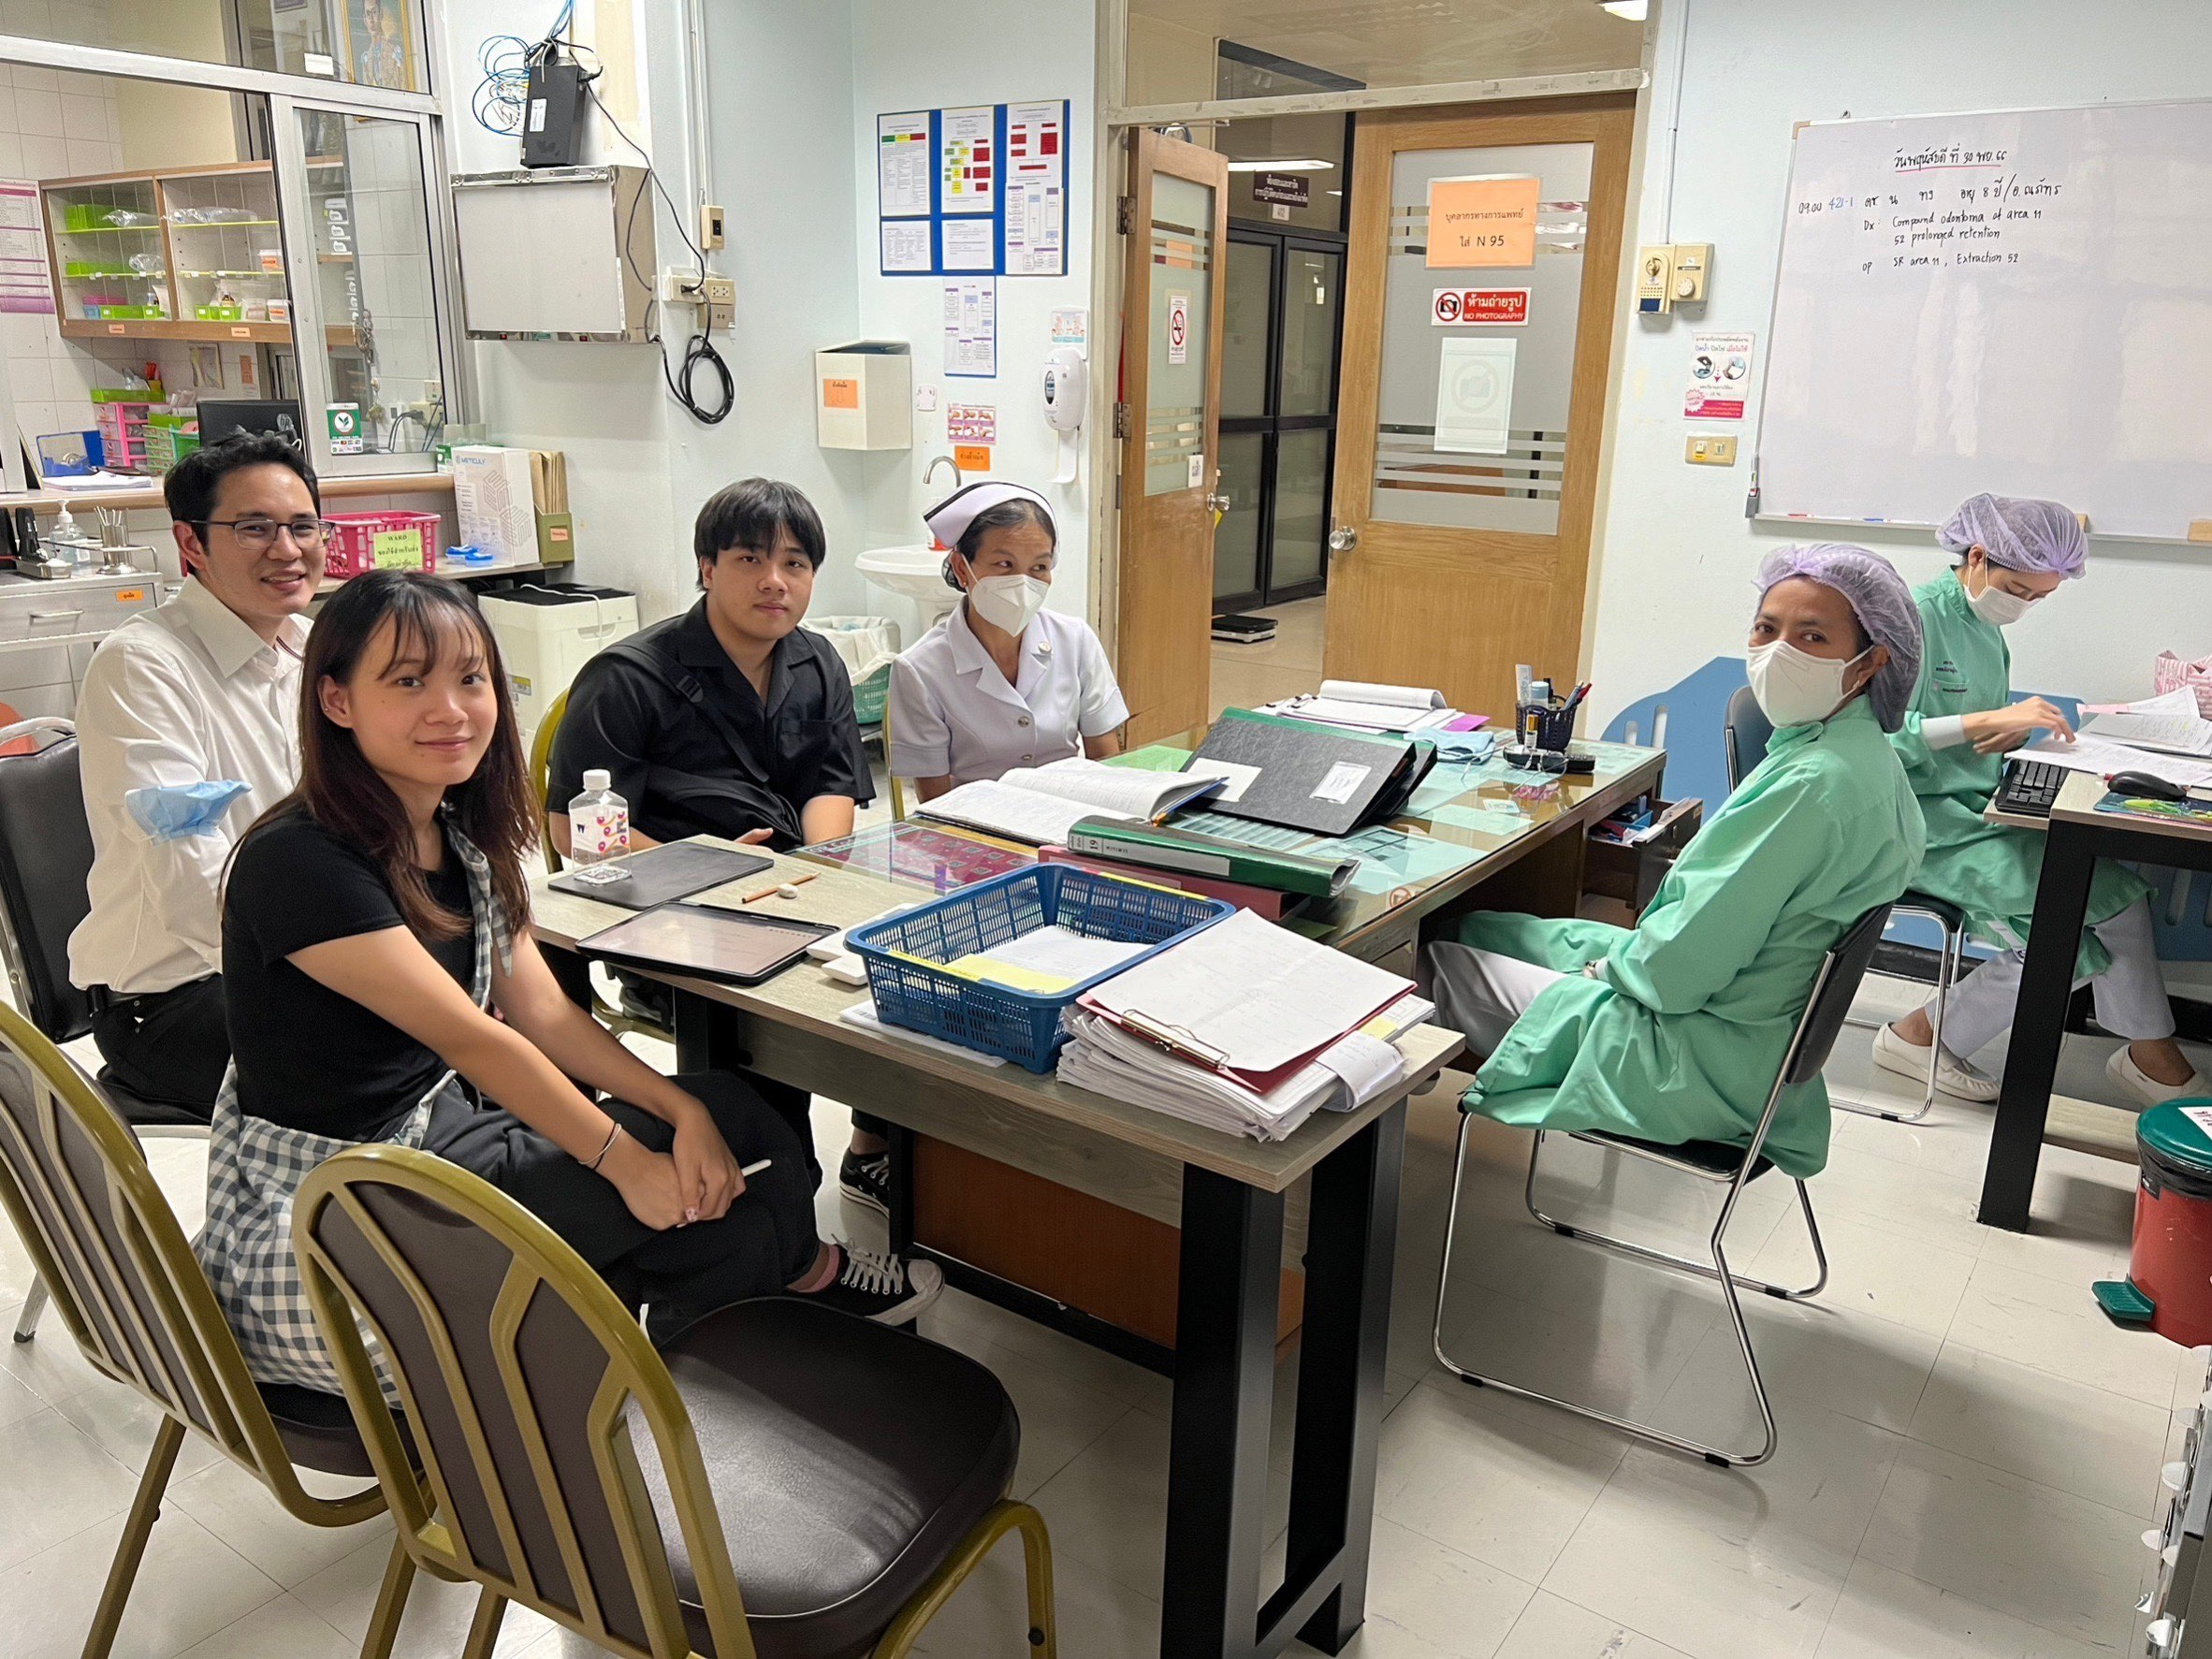
\includegraphics[width=.8\textwidth]{Image/Interview_3.jpg}}
        \caption{Conversation with the nurse who is experienced in the patient follow-up process}\label{fig:Interview_3}
        \begin{flushleft}
          \qquad The follow-up process usually happens three days following a patient's discharge. The nurse will follow-up with the patients and give them advice if needed. \par
        \end{flushleft}
      \end{figure}
      \begin{figure}
        \centering
        \fbox{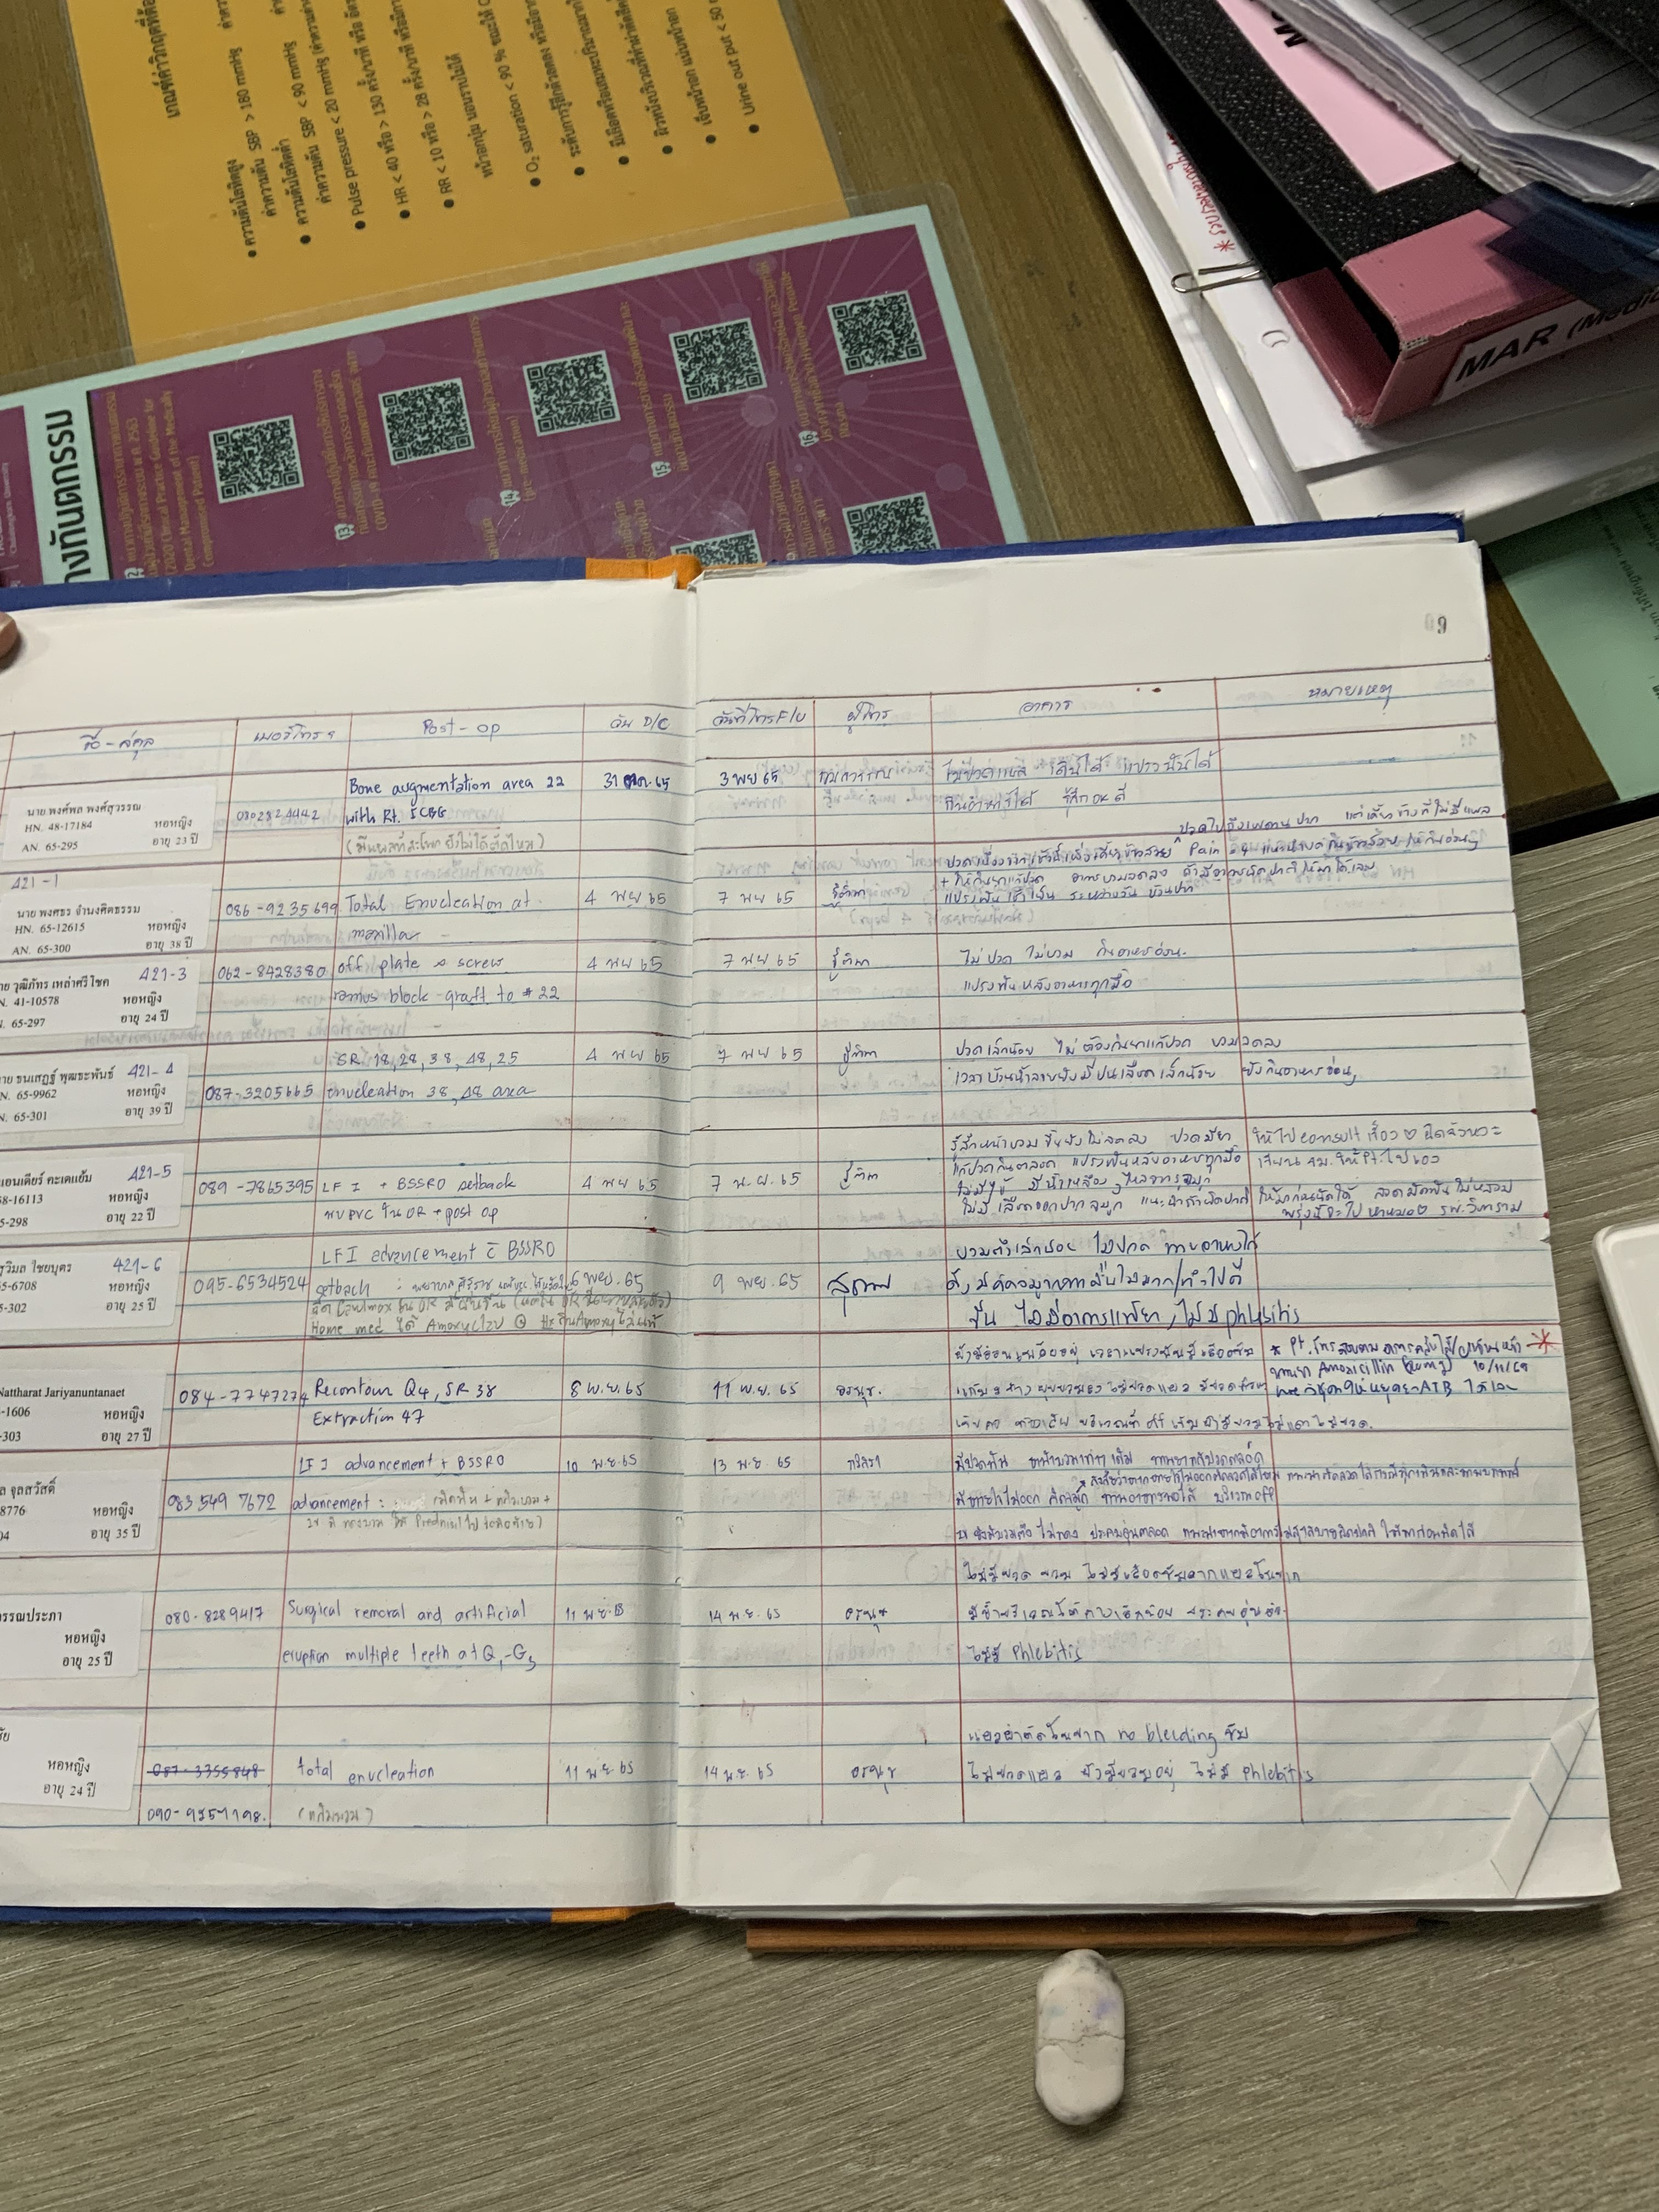
\includegraphics[width=.8\textwidth]{Image/Interview_4.jpg}}
        \caption{Document that the nurse has documented patient information during follow-up sessions}\label{fig:Interview_4}
        \begin{flushleft}
          \qquad The nurse records details such as the operation, discharge date, follow-up date, contact person, symptoms, and any additional notes. This approach is a comprehensive and accurate way of tracking patient data gathered during follow-up calls. \par
        \end{flushleft}
      \end{figure}

%%%%%%%%%%%%%%%%%%%%%%%%%%%%%%%%%%%%%%%%%%%%%%%%%%%%%%%%%%%%%%%
%%%%%%%%%%%%%%%%%%%% Bibliography %%%%%%%%%%%%%%%%%%%%%%%%%%%%%
%%%%%%%%%%%%%%%%%%%%%%%%%%%%%%%%%%%%%%%%%%%%%%%%%%%%%%%%%%%%%%%

%%%% Comment this in your report to show only references you have
%%%% cited. Otherwise, all the references below will be shown.
%\nocite{*}
%% Use the kmutt.bst for bibtex bibliography style 
%% You must have cpe.bib and string.bib in your current directory.
%% You may go to file .bbl to manually edit the bib items.

% Sept, 2021 by Thanin
% improve url breaks to prevent unnecessary big white spaces in some cases
\makeatletter
\g@addto@macro{\UrlBreaks}{\UrlOrds}
\makeatother
% 

\bibliographystyle{kmutt}
\bibliography{string,cpe}
      
\end{document}
